% --- tesi triennale di Giacomo Simonetto ---

% indicazioni sull'impaginazione della tesi richieste dall'università di Padova:
% - https://stem.elearning.unipd.it/mod/book/view.php?id=234&chapterid=46
% - carattere Times New Roman 12
% - interlinea 1,5
% - margini superiore e inferiore di cm. 2, margine esterno di cm. 2, margine interno di cm. 3
% - utilizzare il fac-simile di frontespizio (che è possibile modificare purché vengano mantenute tutte le informazioni
%   presenti nel fac-simile stesso). Il Frontespizio sarà rispettivamente in lingua italiana o lingua inglese in funzione
%   della stesura della tesi.

% documentclass:
% - report: per tesi di laurea con capitoli
% - a4paper: formato A4
% - twoside: i margini interni ed esterni sono scambiati per le pagine "a sinistra" e "a destra"
% - openright: i capitoli cominciano in pagine dispari ("a destra")

% --- 0. TAGGING DOCUMENTI PDF/A ---
\DocumentMetadata{
	pdfstandard = a-2b,      % richiede esplicitamente il PDF/A-2a (livello accessibile)
	lang        = it-IT,     % lingua principale del documento per gli screen reader
	%testphase   = phase-III  % attiva il motore di tagging strutturale per accessibilità (sperimentale ma stabile)
}

% --- 1. PREAMBOLO ---
\documentclass[12pt,a4paper,twoside,openright,italian]{report}

% per gestione dei colori (usata in TikZ, Minted e PDFX)
\usepackage[dvipsnames,rgb]{xcolor}

% corretta sillabazione in italiano
\usepackage{babel}


% --- 2. ENCODING E FONT (Testo) ---
% per utilizzare l'alternativa TeX Gyre Termes con comando pdflatex
\usepackage{cmap}     % rende il testo del PDF ricercabile e copiabile
\usepackage[T1]{fontenc}
\usepackage{lmodern}  % latin modern font for sans-serif and monospace (grafici e verb)
\usepackage{tgtermes} % times new roman-like font for serif (testo principale)

% se il sistema contiene il font times new roman
%\usepackage{fontspec} % per font richiesti dall'università
%\setmainfont{Times New Roman}

% per utilizzare il font times new roman con comando lualatex
%\usepackage{fontspec}
%\setmainfont{TeX Gyre Termes}
%\usepackage{unicode-math}
%\setmathfont{TeX Gyre Termes Math}


% --- 3. AMBIENTE MATEMATICO ---
% per l'ambiente matematico
\usepackage{amsmath}
\usepackage{newtxmath} % per l'ambiente matematico con font TeX Gyre Termes


% --- 4. LAYOUT E GEOMETRIA ---
% per margini richiesti dall'università
\usepackage{geometry}
\geometry{a4paper,top=2cm, bottom=2cm, outer=2cm, inner=3cm, includeheadfoot}

% per interlinea richiesta dall'università
\usepackage{setspace}
\onehalfspacing

% per non spaziare i paragrafi per far arrivare il testo fino a fine pagina
\raggedbottom


% --- 5. GRAFICA, TABELLE E LISTE ---
% immagini
\usepackage{graphicx}
\graphicspath{{./}}

% disegni e schemi
\usepackage{tikz}
\usetikzlibrary{positioning, arrows.meta, shapes.geometric, calc, arrows}

% elenchi puntati
\usepackage{enumitem}
\setlist[itemize]{label=-, topsep=0pt, noitemsep}
\setlist[enumerate]{topsep=0pt, noitemsep}

% tabelle
\usepackage{multirow} % per celle che si espandono su più righe
\usepackage{tabularx} % per tabelle con larghezza flessibile
\usepackage{booktabs} % per linee orizzontali tabelle

% per centrare testo nelle tabelleX
\renewcommand\tabularxcolumn[1]{m{#1}}
\newcolumntype{L}{>{\raggedright\arraybackslash}X}
\newcolumntype{C}{>{\centering\arraybackslash}X}
\newcolumntype{R}{>{\raggedleft\arraybackslash}X}


% --- 6. DIDASCALIE ---
\usepackage{caption} % per le didascalie
\usepackage{subcaption} % per subfigure

% nei codici dei programmi non sono stati usati ambienti flottanti perché altrimenti non sarebbe stato possibile far
% estendere il codice correttamente su più pagine. Inoltre se vengono inseriti caption fuori da ambienti flottanti,
% come avviene nel codice, si generano dei warning di compilazione. Per evitare questi warning, si indica di non
% associare le caption dei listing a un ambiente flottante (cosa che latex tenta di fare in automatico).
%\captionsetup[listing]{hypcap=false}


% --- 7. CODICE SORGENTE ---
% codice tramite pacchetto verbatim per codice + listings per elenco dei codici
%\usepackage{listings}
%\usepackage{verbatim}

% codice tramite pacchetto minted
\usepackage{minted}
% stile del codice sorgente formattato con minted
\setminted{
	linenos=true,          % mostra i numeri di riga
	frame=single,          % riquadro singolo attorno al codice
	framesep=2mm,          % distanza tra il codice e il riquadro
	baselinestretch=0.9,   % interlinea del codice (utile se il documento ha interlinea 1.5)
	fontsize=\tiny,  % dimensione del font più piccola
	breaklines             % wrap automatico delle righe lunghe
}
% stile del codice inline formattato con minted
\setmintedinline{
	fontsize=\normalsize
}

%% codice tramite pacchetto listings
%\usepackage{listings}
%
%% definizione dei colori
%\definecolor{codegreen}{rgb}{0,0.6,0}
%\definecolor{codegray}{rgb}{0.5,0.5,0.5}
%\definecolor{codepurple}{rgb}{0.58,0,0.82}
%\definecolor{backcolour}{rgb}{0.95,0.95,0.92}
%
%% configurazione dello stile
%\lstdefinestyle{mystyle}{
%	backgroundcolor=\color{backcolour},
%	commentstyle=\color{codegreen},
%	keywordstyle=\color{magenta},
%	numberstyle=\tiny\color{codegray},
%	stringstyle=\color{codepurple},
%	basicstyle=\ttfamily\scriptsize,
%	breakatwhitespace=false,
%	breaklines=true,
%	captionpos=t,
%	keepspaces=true,
%	numbers=left,
%	numbersep=5pt,
%	showspaces=false,
%	showstringspaces=false,
%	showtabs=false,
%	tabsize=4,
%	frame=single
%}
%
%\lstset{style=mystyle}

% per tradurre il nome dei listings e dell'elenco dei listings in italiano (minted)
\addto\captionsitalian{%
  \renewcommand{\listingscaption}{Codice}%
  \renewcommand{\listoflistingscaption}{Elenco dei codici}%
}

% per tradurre il nome dei listings e dell'elenco dei listings in italiano (listings o verbatim)
%\addto\captionsitalian{%
%  \renewcommand{\lstlistingname}{Codice}%
%  \renewcommand{\lstlistlistingname}{Elenco dei codici}%
%}


% --- 8. CITAZIONI E BIBLIOGRAFIA ---
\usepackage{xurl} % per spezzare gli url della bibliografia in modo corretto
\usepackage{csquotes} % per le citazioni
\usepackage[backend=biber,style=ieee]{biblatex} % per la bibliografia
\addbibresource{bibliografia.bib}

% Forza BibLaTeX a spezzare gli URL su lettere maiuscole, minuscole e numeri
\setcounter{biburlnumpenalty}{7000}
\setcounter{biburllcpenalty}{7000}
\setcounter{biburlucpenalty}{8000}


% --- 9. STANDARD PDF/A E LINK IPERTESTUALI ---
%\usepackage[a-1b]{pdfx} % per creare un documento PDF/A-1a
\usepackage{hyperref} % per link ipertestuali

% per autoref dei listing
\providecommand*{\listingautorefname}{codice} % minted
%\providecommand*{\lstlistingautorefname}{codice} % listings o verbatim

% per metadati PDF/A richiesti dall'università
\hypersetup{
	colorlinks=true,       % Sostituisce i riquadri con il testo colorato
    linkcolor=black,       % Colore dei riferimenti interni (capitoli, figure, equazioni)
    citecolor=black,       % Colore delle citazioni bibliografiche
    urlcolor=NavyBlue,     % Colore dei link web esterni
	pdftitle={Sviluppo firmware per la gestione del sistema di riscaldamento di un prototipo di incubatrice neonatale},
	pdfauthor={Giacomo Simonetto},
	pdfsubject={Tesi triennale},
	pdfkeywords={firmware, microcontrollore, incubatrice, temperatura, pid}
}

% --- 10. DATI PER FRONTESPIZIO ---
\title{Sviluppo firmware per la gestione del sistema di riscaldamento di un prototipo di incubatrice neonatale}
\author{Simonetto Giacomo}
\date{22/09/2026}
\newcommand{\supervisor}{Prof. Rampazzo Mirco}
\newcommand{\matricola}{2109923}


% --- 11. DOCUMENTO ---
\begin{document}
	\pagenumbering{roman}
	\pagestyle{empty} % per le prime pagine, non mostrare il numero di pagina

	\begin{titlepage}
	% solo il frontespizio deve essere simmetrico rispetto ai margini interno ed esterno
	\newgeometry{hmargin=2.5cm,vmargin=2cm}

	\begin{center}
		\begin{minipage}{0.45\textwidth}
			\raggedright
			
\includegraphics[height=3cm]{immagini/logo_unipd.pdf}
		\end{minipage}
		\hfill
		\begin{minipage}{0.4\textwidth}
			\raggedleft
			
\includegraphics[height=2.5cm]{immagini/logo_dei.pdf}
		\end{minipage}
	\end{center}

	\vspace{\stretch{0.5}}

	\begin{center}
		\makeatletter % serve per poter usare \@...

		UNIVERSITÀ DEGLI STUDI DI PADOVA \\
		\vspace*{\stretch{0.1}}
		DIPARTIMENTO DI INGEGNERIA DELL'INFORMAZIONE \\


		\vspace*{\stretch{0.5}}
		\LARGE
		\textbf{\@title}

		\vspace*{\stretch{1}}
		\normalsize
		\begin{tabular*}{\textwidth}{l @{\extracolsep{\fill}} r}
			\textbf{Relatore} & \textbf{Laureando} \\
			\supervisor       & \@author \\
			& \matricola \\
			\textbf{Correlatore} \\
			\assistantsupervisor \\
		\end{tabular*}

		\vspace*{\stretch{2}}
		\text{ANNO ACCADEMICO 2025-2026} \\
		\vspace*{\stretch{0.1}}
		Data di laurea \@date

		\makeatother % serve dopo \makeatletter
	\end{center}
	\restoregeometry
\end{titlepage}

	\cleardoublepage

	\vspace*{\stretch{0.8}}
Alla mia famiglia e ai miei amici.
\vspace*{\stretch{1}}

	\cleardoublepage

	\pagestyle{plain} % comincia a mostrare il numero di pagina
	\phantomsection
	\addcontentsline{toc}{chapter}{Abstract}
	\chapter*{Abstract}
La presente tesi descrive lo sviluppo di un firmware per la gestione del sistema di riscaldamento e umidificazione e la verifica
del corretto funzionamento dei singoli componenti del prototipo di incubatrice neonatale costruita da Vanni Bincoletto per la
sua tesi magistrale \cite{bincoletto2025}

	\cleardoublepage

	\tableofcontents
	\cleardoublepage

	\phantomsection
	\addcontentsline{toc}{chapter}{\listfigurename}
	\listoffigures
	\cleardoublepage

	\phantomsection
	\addcontentsline{toc}{chapter}{\listtablename}
	\listoftables
	\cleardoublepage

	\phantomsection
	\addcontentsline{toc}{chapter}{Elenco dei codici}
	\listoflistings % minted
	%\lstlistoflistings % listings o verbatim
	\cleardoublepage

	\pagenumbering{arabic}

	\chapter{Introduzione}
\section{Contesto e funzione di una incubatrice neonatale}
\subsection{Esigenze dei neonati prematuri}
Con il termine di ``neonati prematuri'' si intendono tutti i bambini nati prima della 37\textsuperscript{a} settimana di
gestazione. A causa del loro mancato sviluppo, non dispongono di un sistema di termoregolazione adeguato a mantenere la
temperatura corporea ideale compresa tra i 36,5 °C e i 37,5 °C. Già quando scende al di sotto dei 36°C, il neonato entra
in una fase di ipotermia e se tale condizione si protrae nel tempo, si possono verificare gravi conseguenze sulla salute
del neonato, fino a portarlo alla morte.

Si identifica la temperatura critica come la temperatura a cui un essere umano non è più in grado di regolare la propria
temperatura corporea. Per un adulto si aggira attorno agli 0°C mentre per un neonato prematuro è compresa tra i 20°C e
i 23°C. Dato che questo valore è particolarmente elevato, casi di ipotermia sono molto frequenti nei neonati prematuri
in qualsiasi parte del mondo, anche nei paesi tropicali.

Per mantenere il neonato in condizioni di salute ottimali, risulta, quindi, necessario adottare misure per limitare
la dispersione di calore. Queste possono essere semplici azioni fattibili da chiunque, come il mantenimento del neonato
asciutto ed avvolto da indumenti caldi, oppure il metodo canguro-madre che consiste nel contatto pelle a pelle tra il
neonato e la madre. In alternativa esistono soluzioni più avanzate come l'uso di incubatrici neonatali o culle riscaldate,
in grado di mantenere una temperatura costante e confortevole per il neonato. \cite{world1993thermal}

\subsection{Storia delle incubatrici neonatali}
La prima idea di incubatrice neonatale venne proposta nel 1857 da Jean-Louis-Paul Denucé (1824 - 1889), un medico belga,
che, per mantenere in vita (purtroppo invano) un neonato prematuro, per primo costruì e descrisse formalmente una
culla di metallo a doppia parete senza coperchio superiore, in cui, nella cavità tra le due pareti, veniva versata acqua
calda. Tale struttura di incubatrice, però, non ebbe grande diffusione.

Nel 1881, un medico francese, Stéphane Tarnier (1828 - 1897), durante una visita allo Zoo di Parigi notò un'incubatrice
chiusa usata per le uova di uccelli e subito ne intuì le potenzialità per i neonati prematuri. Fece costruire un
modello simile con pareti in legno, un compartimento inferiore per contenere l'acqua calda e introdusse per la prima volta
il coperchio in vetro rendendola chiusa e più efficace. La struttura di Tarnier venne poi resa più semplice ed economica
da Alfred Auvard (1855-1940) negli anni successivi, rendendola più accessibile agli ospedali e favorendone la rapida
diffusione. Grazie a questo modello, Tarner riuscì a far aumentare la probabilità di sopravvivenza dei neonati di peso
inferiore ai 2kg dal 35\% al 62\%. \cite{DunnF137}

Poco più tardi, il medico americano Joseph Bolivar DeLee (1869 - 1942), nel 1899 durante il suo servizio presso il Chicago
Lying-In Hospital, notò la necessità di dover fornire assistenza tempestiva e sul posto ai neonati prematuri, che nascevano
a casa. Decise, quindi, di modificare il modello di Auvard per creare la prima incubatrice portatile, facilmente trasportabile
dall'ospedale al domicilio del neonato.

Ad oggi le incubatrici neonatali sono molto diffuse ed utilizzate. Sono costruite da una struttura trasparente di policarbonato
con delle aperture per l'accesso rapido al neonato. Dispongono di sistemi di riscaldamento, ventilazione e umidificazione,
oltre che a numerosi sensori per controllare lo stato dell'incubatrice e del neonato e a sistemi di allarme per segnalare
eventuali malfunzionamenti o criticità.

\section{Obiettivi della tesi}
L'obiettivo principale di questa tesi consiste nel rendere completamente funzionante il prototipo di incubatrice neonatale
costruito da Vanni Bincoletto nella sua tesi magistrale in bioingegneria \cite{bincoletto2025} e sviluppare un sistema di
gestione della temperatura.


\begin{itemize}
	\item sviluppo multidisciplinare e trasversale (hardware, software, controllore)
	\item mettere in pratica le conoscenze teoriche viste a lezione
	\item verificare l'efficacia dei controllori pid per il controllo della temperatura
\end{itemize}

\section{Struttura dell'elaborato}
Il seguente elaborato è organizzato in quattro capitoli principali, oltre al primo capitolo di introduzione. In ognuno di
essi viene trattato un argomento specifico corrispondente ad una fase dello sviluppo del prototipo di incubatrice neonatale.

Nel secondo capitolo vengono descritti i vari componenti elettronici del prototipo come il microcontrollore, i sensori
ed i vari attuatori. Vengono inoltre presentate le connessioni realizzate tra di essi per garantire il corretto funzionamento
di ogni componente del sistema.

Nel terzo capitolo si affronta lo sviluppo del firmware per il microcontrollore. Vengono enunciati i requisiti che hanno
guidato le scelte implementative e si analizzano i vari moduli in cui è stato suddiviso il codice.

Nel quarto capitolo si tratta del sistema di controllo usato per la gestione della temperatura. Viene prima descritto un
semplice controllore ad isteresi e successivamente si passa ad un controllore PID. Si conclude con un confronto tra i due
metodi di controllo, evidenziando i vantaggi, gli svantaggi ed i limiti di ognuno.

Nel quinto capitolo si discutono in maniera critica i risultati raggiunti rispetto agli obiettivi prefissati all'inizio
e si propongono possibili sviluppi futuri per migliorare ulteriormente il prototipo di incubatrice neonatale.

A concludere è presente un'appendice in cui sono riportati la dimostrazione matematica di una formula usata nel controllore
PID e il codice sorgente completo del firmware.

In questa tesi verrà analizzata esclusivamente la gestione del sistema di riscaldamento. Poiché, tuttavia, il prototipo
di incubatrice neonatale è dotato anche di un umidificatore, è stata prevista la possibilità di implementare in futuro
un sistema di controllo dell’umidità. A tal fine, il possibile utilizzo dell’umidificatore è stato considerato sia nella
progettazione della circuiteria hardware sia nello sviluppo del software, senza implementare un valido sistema di controllo
dedicato alla gestione dell’umidità.

	\cleardoublepage

	\chapter{Sviluppo dell'hardware dell'incubatrice neonatale}
\section{Architettura del sistema}
In questo capitolo vengono descritte le caratteristiche fisiche del prototipo di incubatrice neonatale. Si parte dalla descrizione
della struttura fisica, si prosegue con la descrizione dei componenti elettronici presenti ed infine si analizzano le connessioni
tra i vari componenti e il microcontrollore. Per una migliore organizzazione, l'insieme delle componenti elettriche
ed elettroniche è stato suddiviso in tre macrocategorie, affrontate nei successivi paragrafi:
\begin{enumerate}
	\item attuatori e relè;
	\item pannello frontale e sensore di temperatura e umidità SHT20;
	\item scheda Arduino Mega 2560 con microcontrollore ATmega2560.
\end{enumerate}


\subsection{Descrizione della struttura fisica}
L'incubatrice neonatale è composta da una camera interna principale ed un cassetto inferiore contenente i componenti elettronici
e la vasca con l'acqua per l'umidificazione.

La camera interna è costituita con pareti laterali in polistirene espanso sinterizzato (ESP) sostenute ai quattro angoli da un
telaio in legno. La base della camera interna è costituita da un pannello in legno ed è stato usato un pannello in policarbonato
trasparente come rivestimento superiore. Il pannello superiore è incernierato alla struttura in legno lungo il lato lungo e
permette il rapido accesso alla camera interna. Sul lato frontale sono presenti due sportelli che permettono un accesso rapido
alla camera interna senza provocare grandi dispersioni di calore e umidità.

Il cassetto inferiore è realizzato con una struttura in legno estraibile dove sono posizionati i vari componenti elettronici
e la vasca con l'acqua per l'umidificazione.

\begin{figure}[htbp]
	\centering
	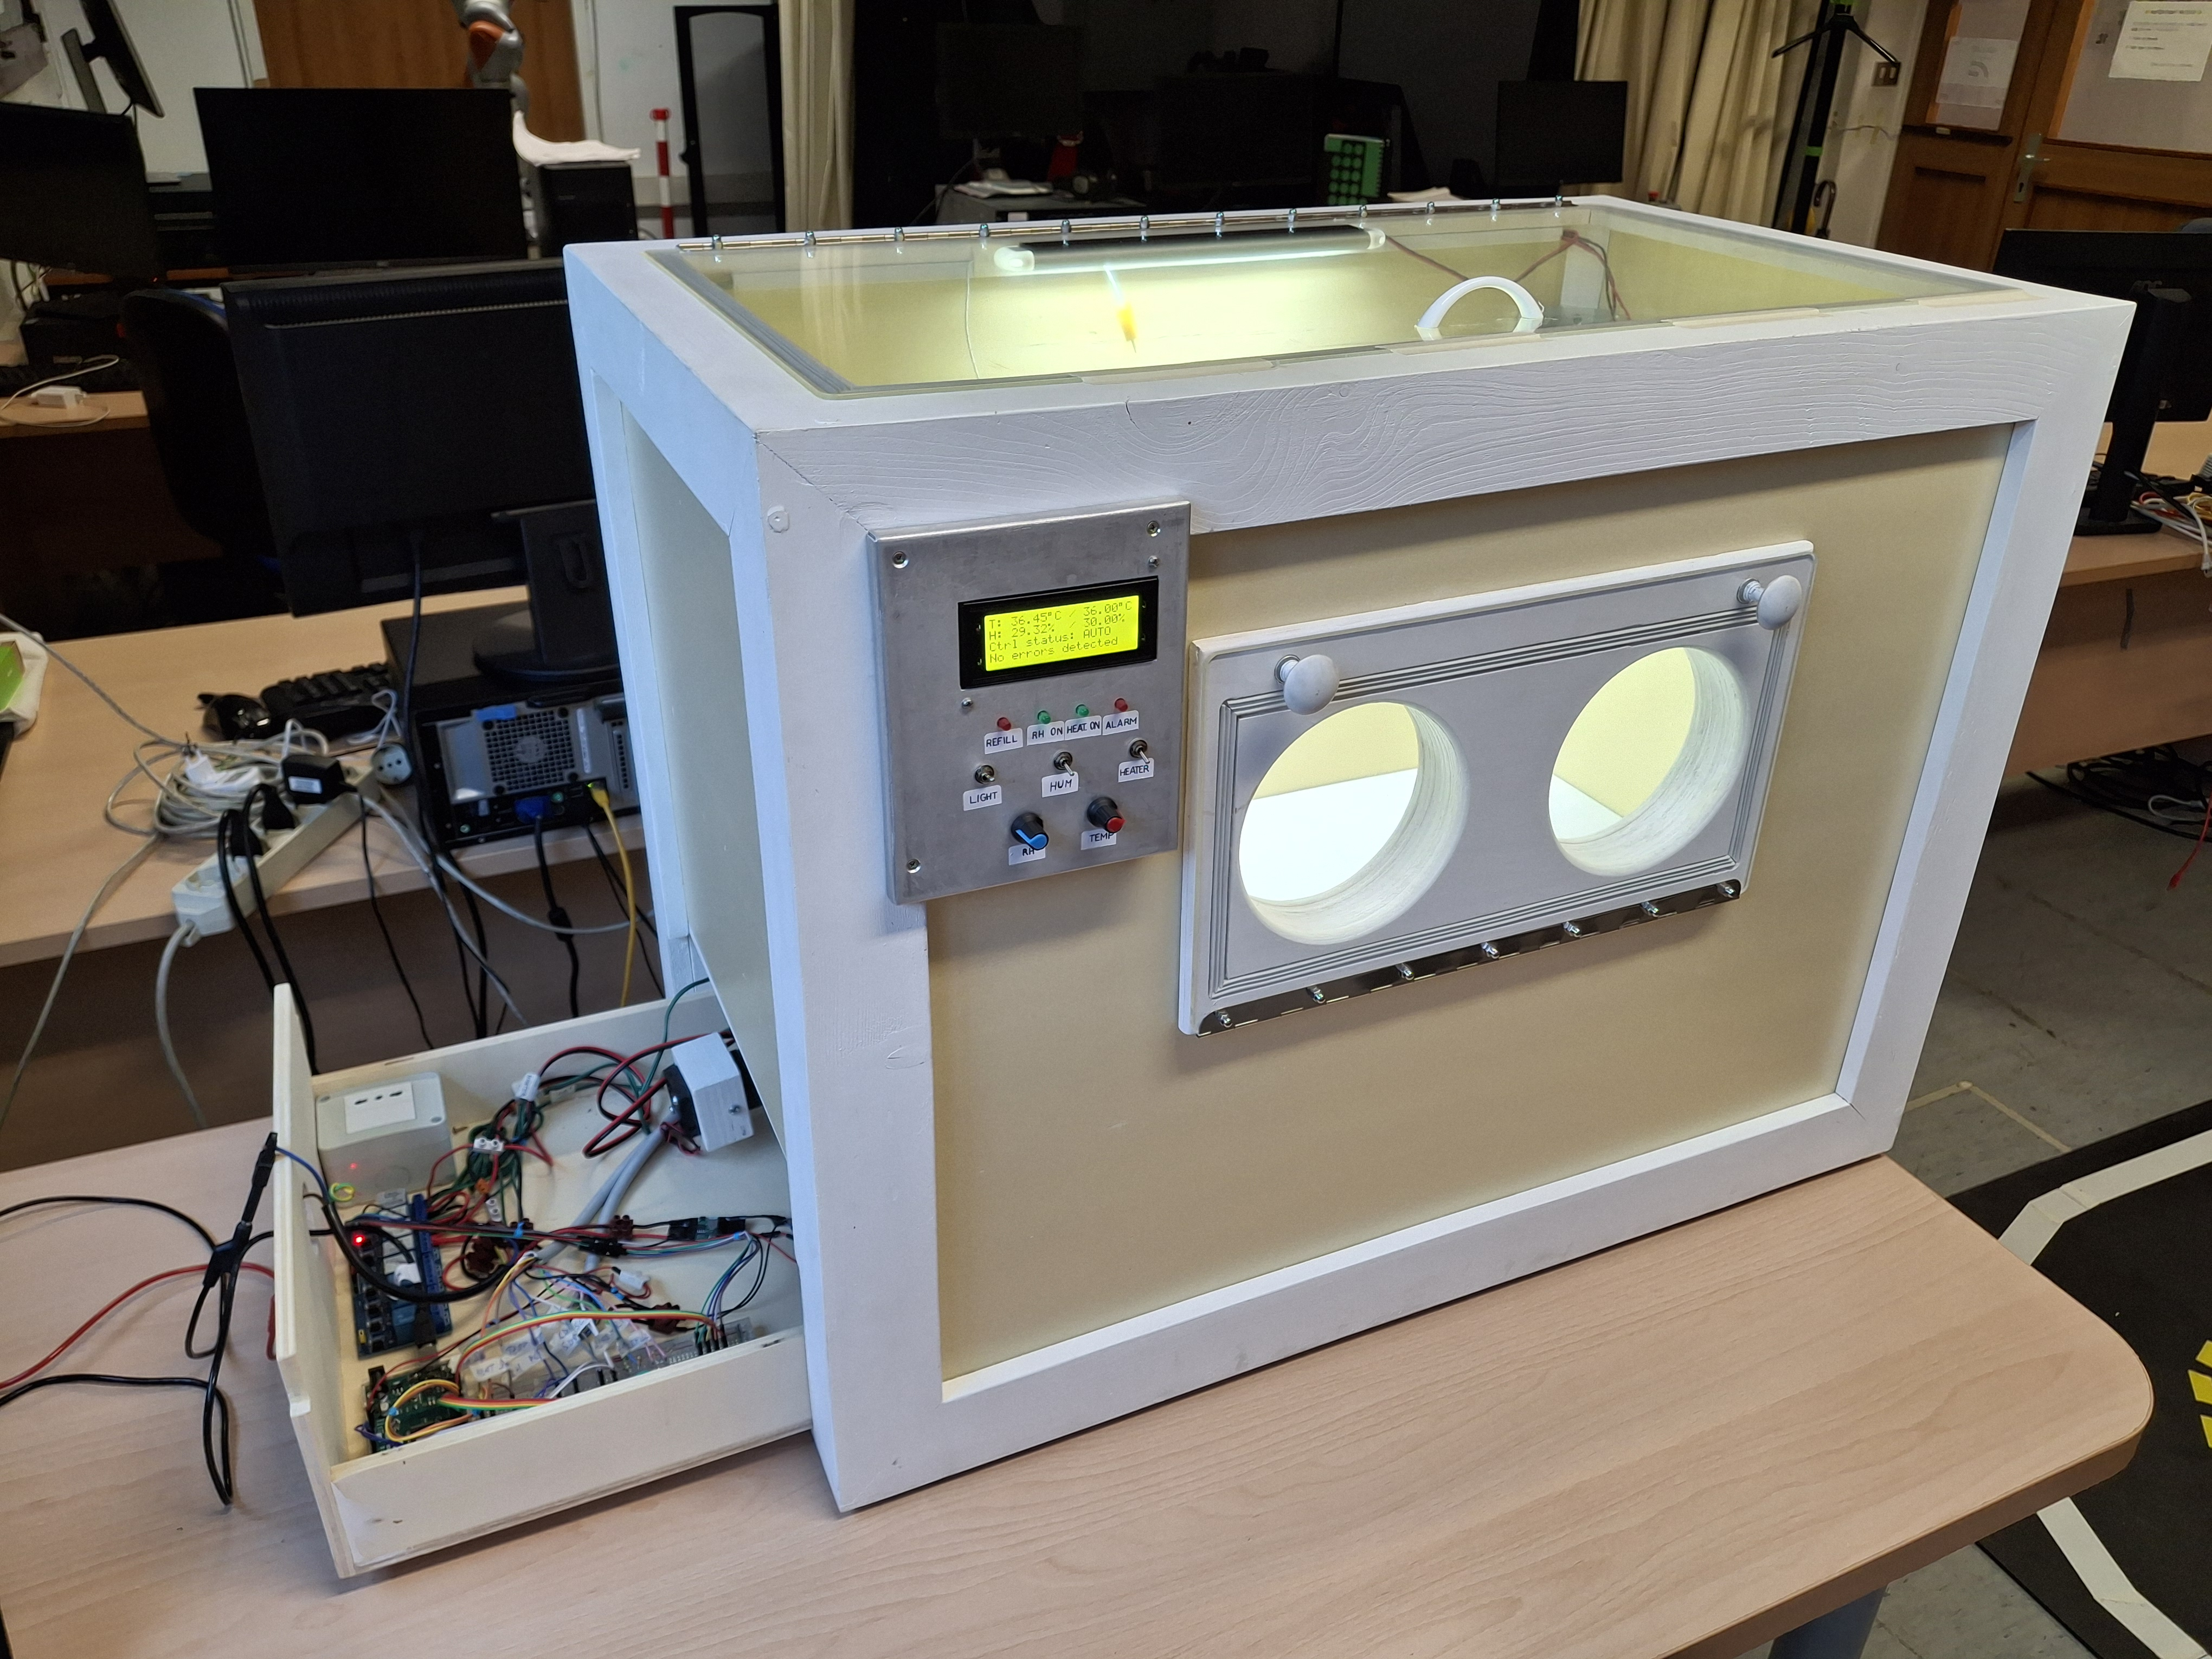
\includegraphics[width=0.9\textwidth, trim={0cm 7cm 0cm 8cm}, clip]{immagini/1_incubatrice.jpg}
	\caption[Foto del prototipo di incubatrice neonatale]{Foto del prototipo di incubatrice neonatale dove si può apprezzare
	la camera interna illuminata, il cassetto inferiore con i componenti elettronici, i due oblò per l'accesso rapido, il
	pannello in policarbonato superiore e il pannello frontale.}
	\label{fig:interno_incubatrice}
\end{figure}

\subsection{Attuatori e relè}
Di seguito sono analizzati i vari attuatori presenti nel prototipo di incubatrice neonatale che permettono di agire sul sistema
per modificarne le condizioni ambientali interne.

\subsubsection{Riscaldatore con ventola associata}
Per riscaldare l'aria della camera interna, è utilizzato un riscaldatore a resistenza elettrica da 100W. Esso è situato
su un angolo della camera interna e sorretto da un supporto in alluminio attaccato al telaio in legno. Dietro al riscaldatore è
presente una ventola che permette di spingere l'aria attraverso le resistenze elettriche del riscaldatore.

\subsubsection{Umidificatore con ventola associata}
Per l'umidificazione dell'aria della camera interna, si utilizza un umidificatore a ultrasuoni per generare vapore acqueo. Si trova
nel cassetto inferiore all'interno di un contenitore in plastica ermetico che funge da serbatoio dell'acqua. Il vapore acqueo
prodotto viene spinto dalla ventola all'interno di un tubo in plastica che collega il contenitore con la camera interna.

\subsubsection{Ventola di omogeneizzazione dell'aria}
Per favorire il ricircolo dell'aria nella camera interna, ed evitare la formazione di stratificazioni di temperatura e umidità,
è presente una ventola di omogeneizzazione dell'aria. Si trova sull'angolo adiacente al riscaldatore ed è anch'essa sorretta da
un supporto in alluminio.

\subsubsection{Barra led}
Per l'illuminazione della camera interna, è presente una barra led posta sul pannello trasparente superiore della camera interna.

\subsubsection{Relè e step down per il controllo degli attuatori}
I vari attuatori con le relative ventole sopra elencati richiedono tutti una tensione di alimentazione di 12 V. L'unico che fa
eccezione è l'umidificatore che lavora a 24 V. Date le elevate correnti richieste, per garantire un funzionamento stabile e sicuro
i vari gli attuatori a 12 V sono collegati ad un alimentatore da banco esterno opportunamente dimensionato, mentre l'umidificatore
è alimentato dal suo alimentatore esterno da 24V.

Per poter essere gestiti dal microcontrollore, tra l'alimentatore e i vari attuatori, sono stati inseriti dei relè controllati
con segnali a 5 V dalla scheda Arduino Mega. Siccome le bobine dei relè richiedono una corrente maggiore di quella che può essere
erogata dal microcontrollore, è stato aggiunto un convertitore step down da 12 V a 5 V per alimentare le bobine dei relè a 5 V
utilizzando l'energia erogata dall'alimentatore esterno a 12 V.

\begin{figure}[htbp]
    \centering
    \begin{subfigure}[b]{0.48\textwidth}
        \centering
        %
\includegraphics[width=\textwidth]{1_riscaldatore.jpg}
        \caption{Riscaldatore a resistenza elettrica con ventola posta dietro di esso.}
        \label{fig:riscaldatore}
    \end{subfigure}
    \hfill % Spinge le immagini verso i margini, creando spazio al centro
    \begin{subfigure}[b]{0.48\textwidth}
        \centering
        %\includegraphics[width=\textwidth]{2_umidificatore.jpg}
        \caption{Umidificatore a ultrasuoni con ventola per spingere il vapore acqueo verso la camera interna.}
        \label{fig:umidificatore}
    \end{subfigure}
    \vspace{0.5cm}
	\begin{subfigure}[b]{0.48\textwidth}
        \centering
        %
\includegraphics[width=\textwidth]{1_ventola_omogeneizzazione.jpg}
        \caption{Ventola di omogeneizzazione dell'aria per favorire il ricircolo dell'aria nella camera interna.}
        \label{fig:ventola_omogeneizzazione}
    \end{subfigure}
    \hfill
    \begin{subfigure}[b]{0.48\textwidth}
        \centering
        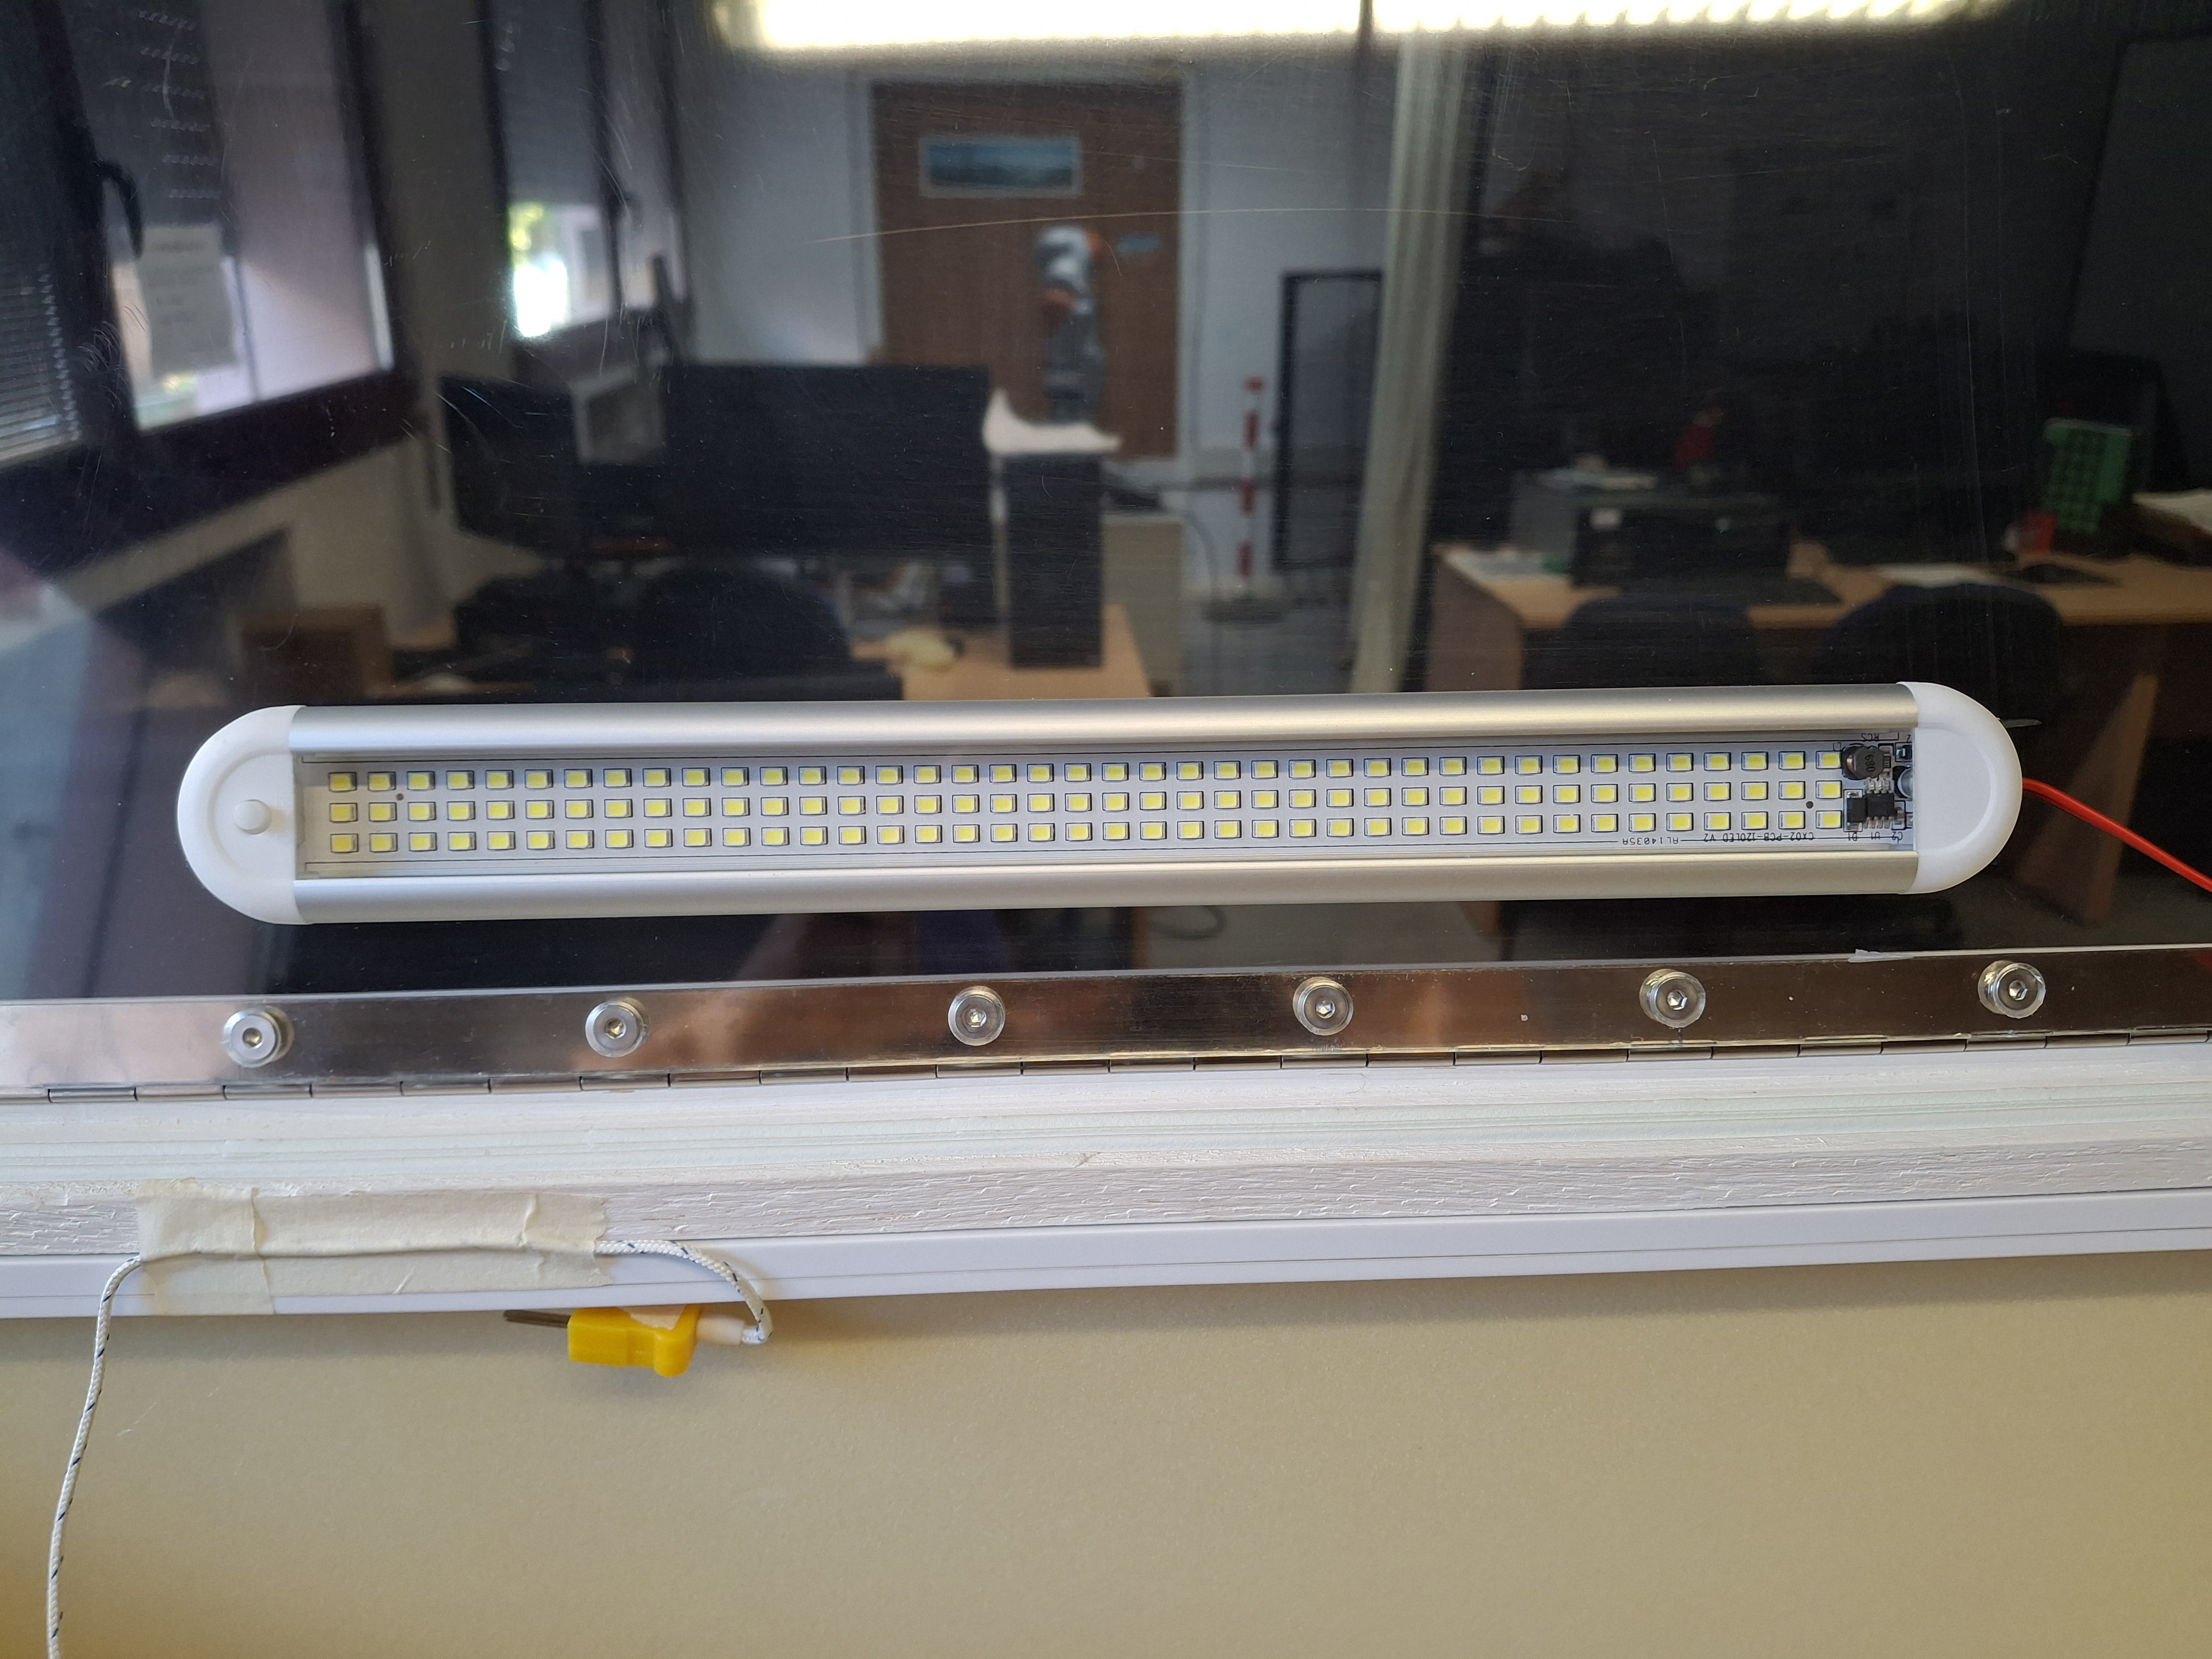
\includegraphics[width=0.9\textwidth, trim={0cm 25cm 0cm 25cm}, clip]{immagini/1_barra_led.jpg}
        \caption{Barra LED per l'illuminazione della camera interna.}
        \label{fig:barra_led}
    \end{subfigure}

    \caption[Foto degli attuatori]{Foto degli attuatori presenti nel prototipo di incubatrice neonatale.}
    \label{fig:griglia_completa}
\end{figure}

\begin{figure}[htbp]
	\centering
	\begin{subfigure}[b]{0.65\textwidth}
        \centering
		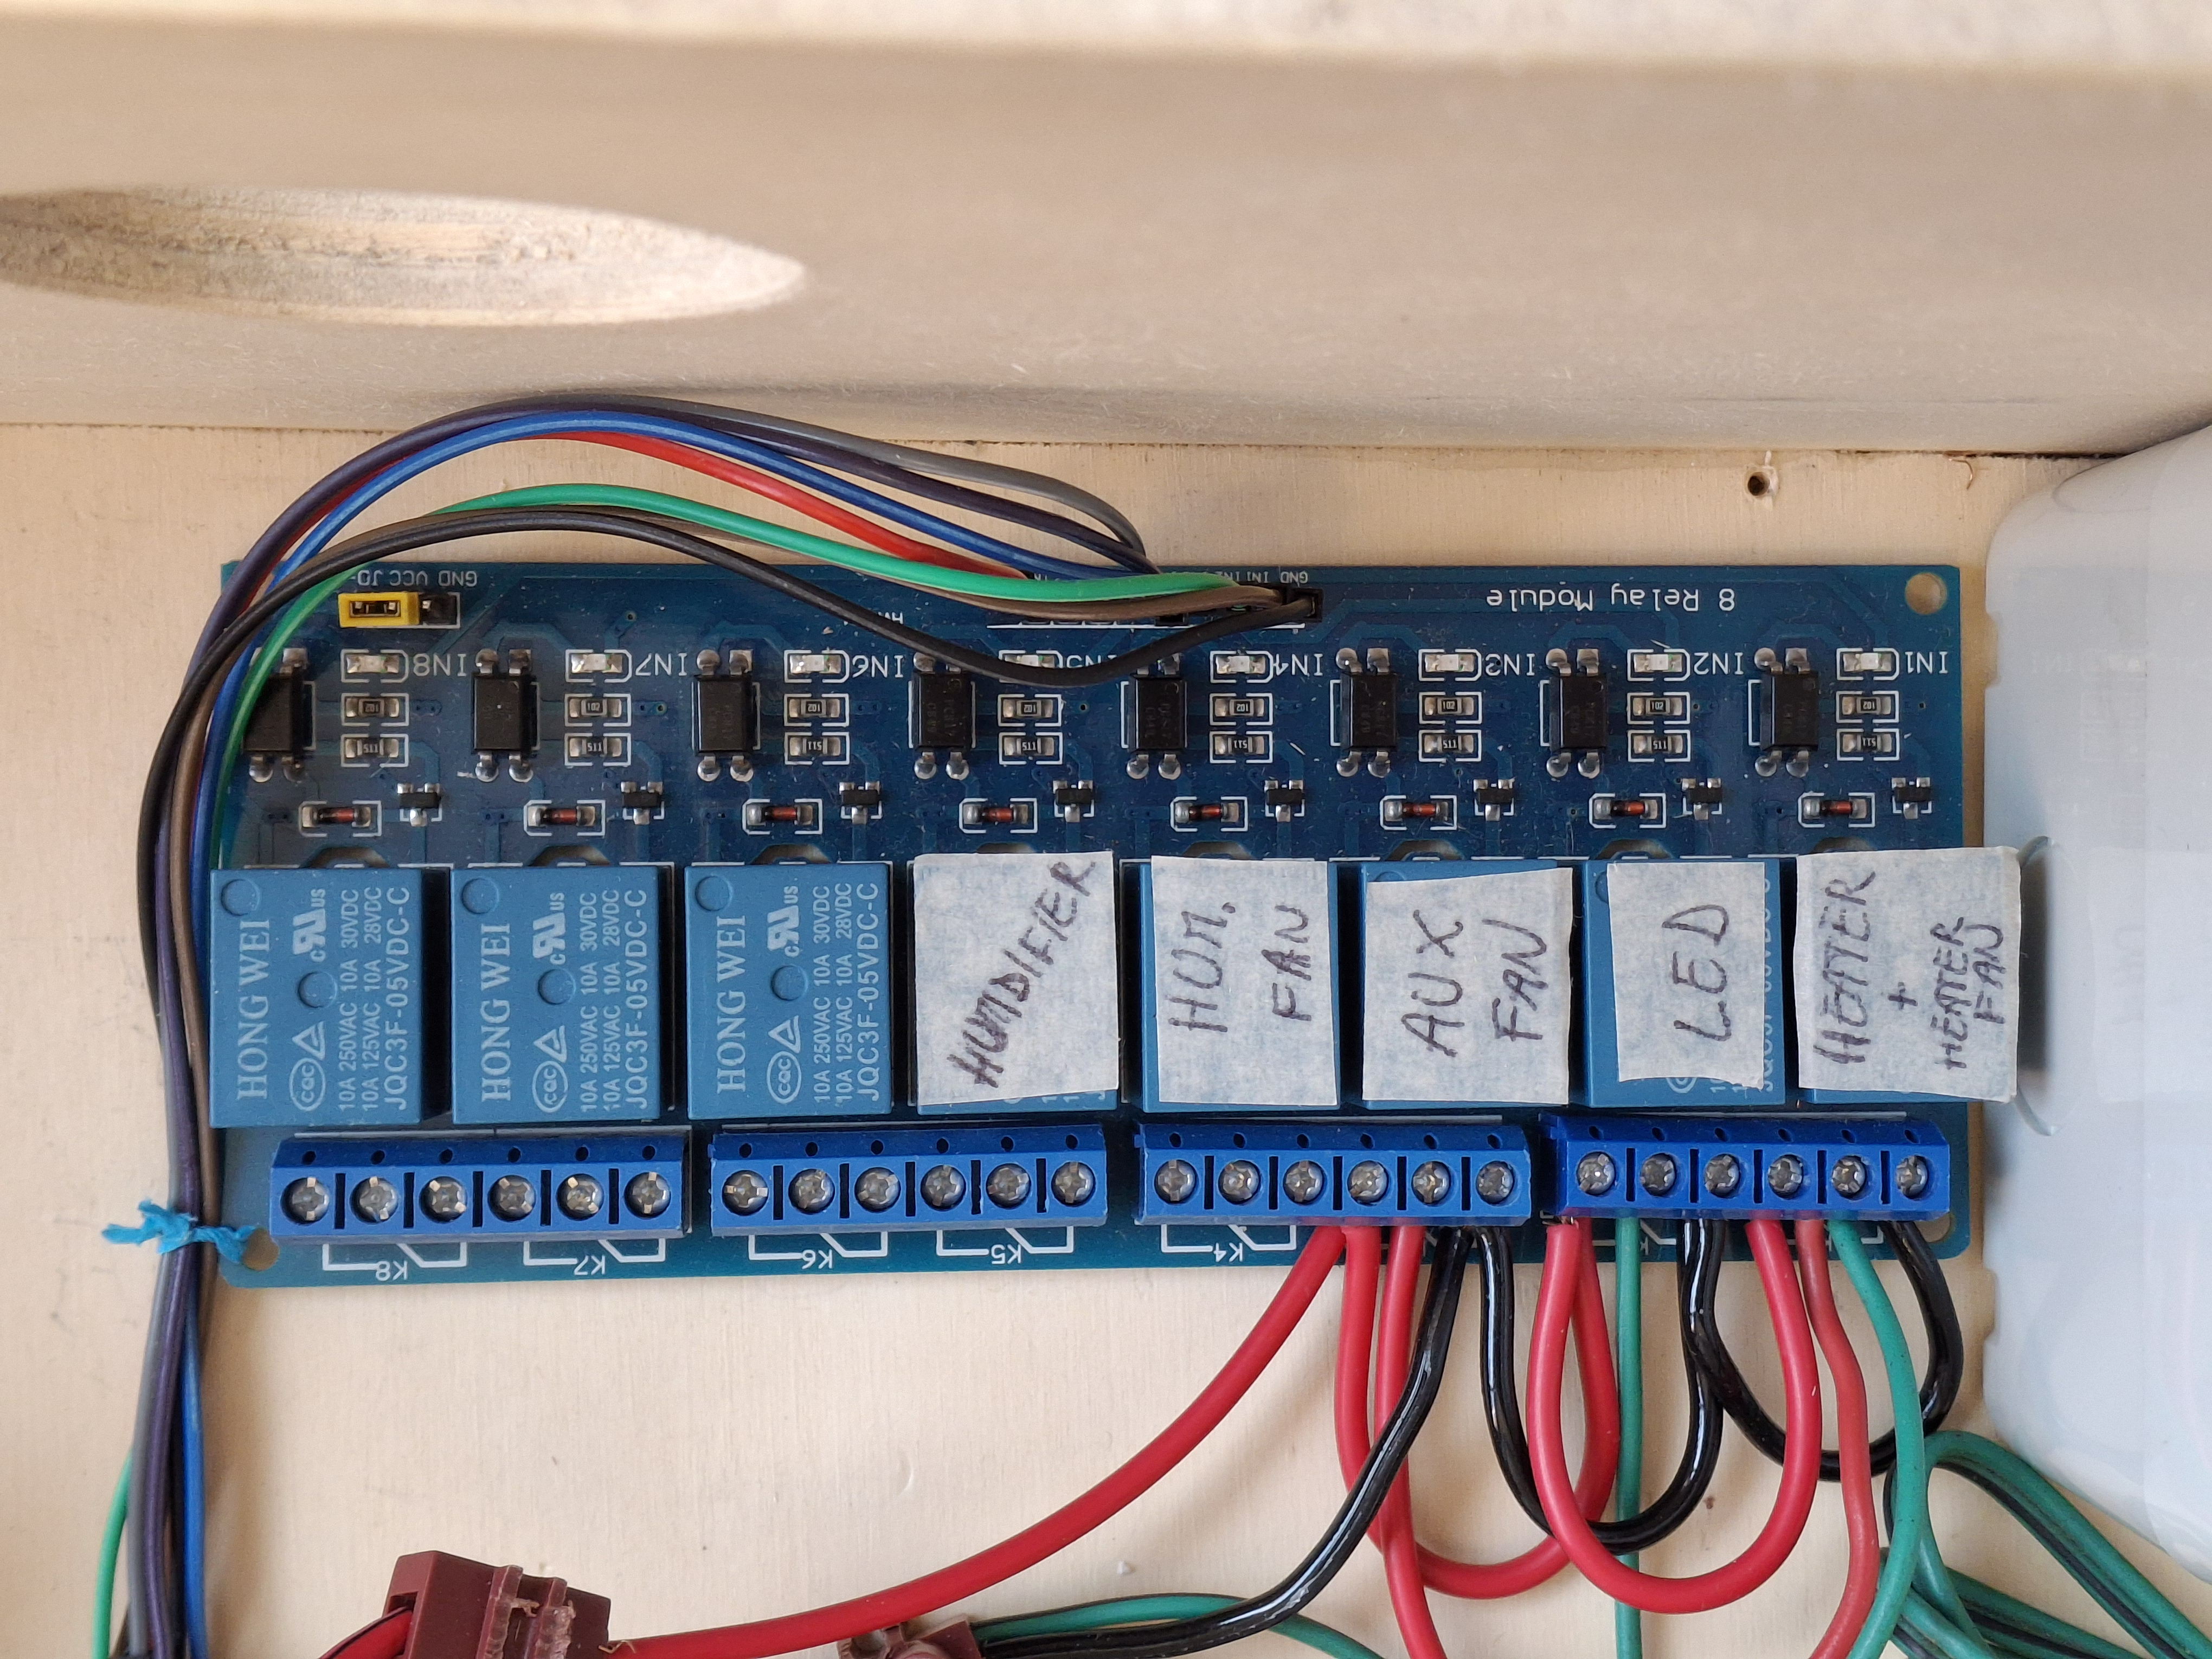
\includegraphics[width=0.9\textwidth, trim={1cm 2cm 2cm 20cm}, clip]{immagini/1_rele.jpg}
        \caption{Foto dei relè per il controllo degli attuatori del prototipo di incubatrice neonatale.}
        \label{fig:rele}
    \end{subfigure}
    \hfill % Spinge le immagini verso i margini, creando spazio al centro
    \begin{subfigure}[b]{0.34\textwidth}
        \centering
        %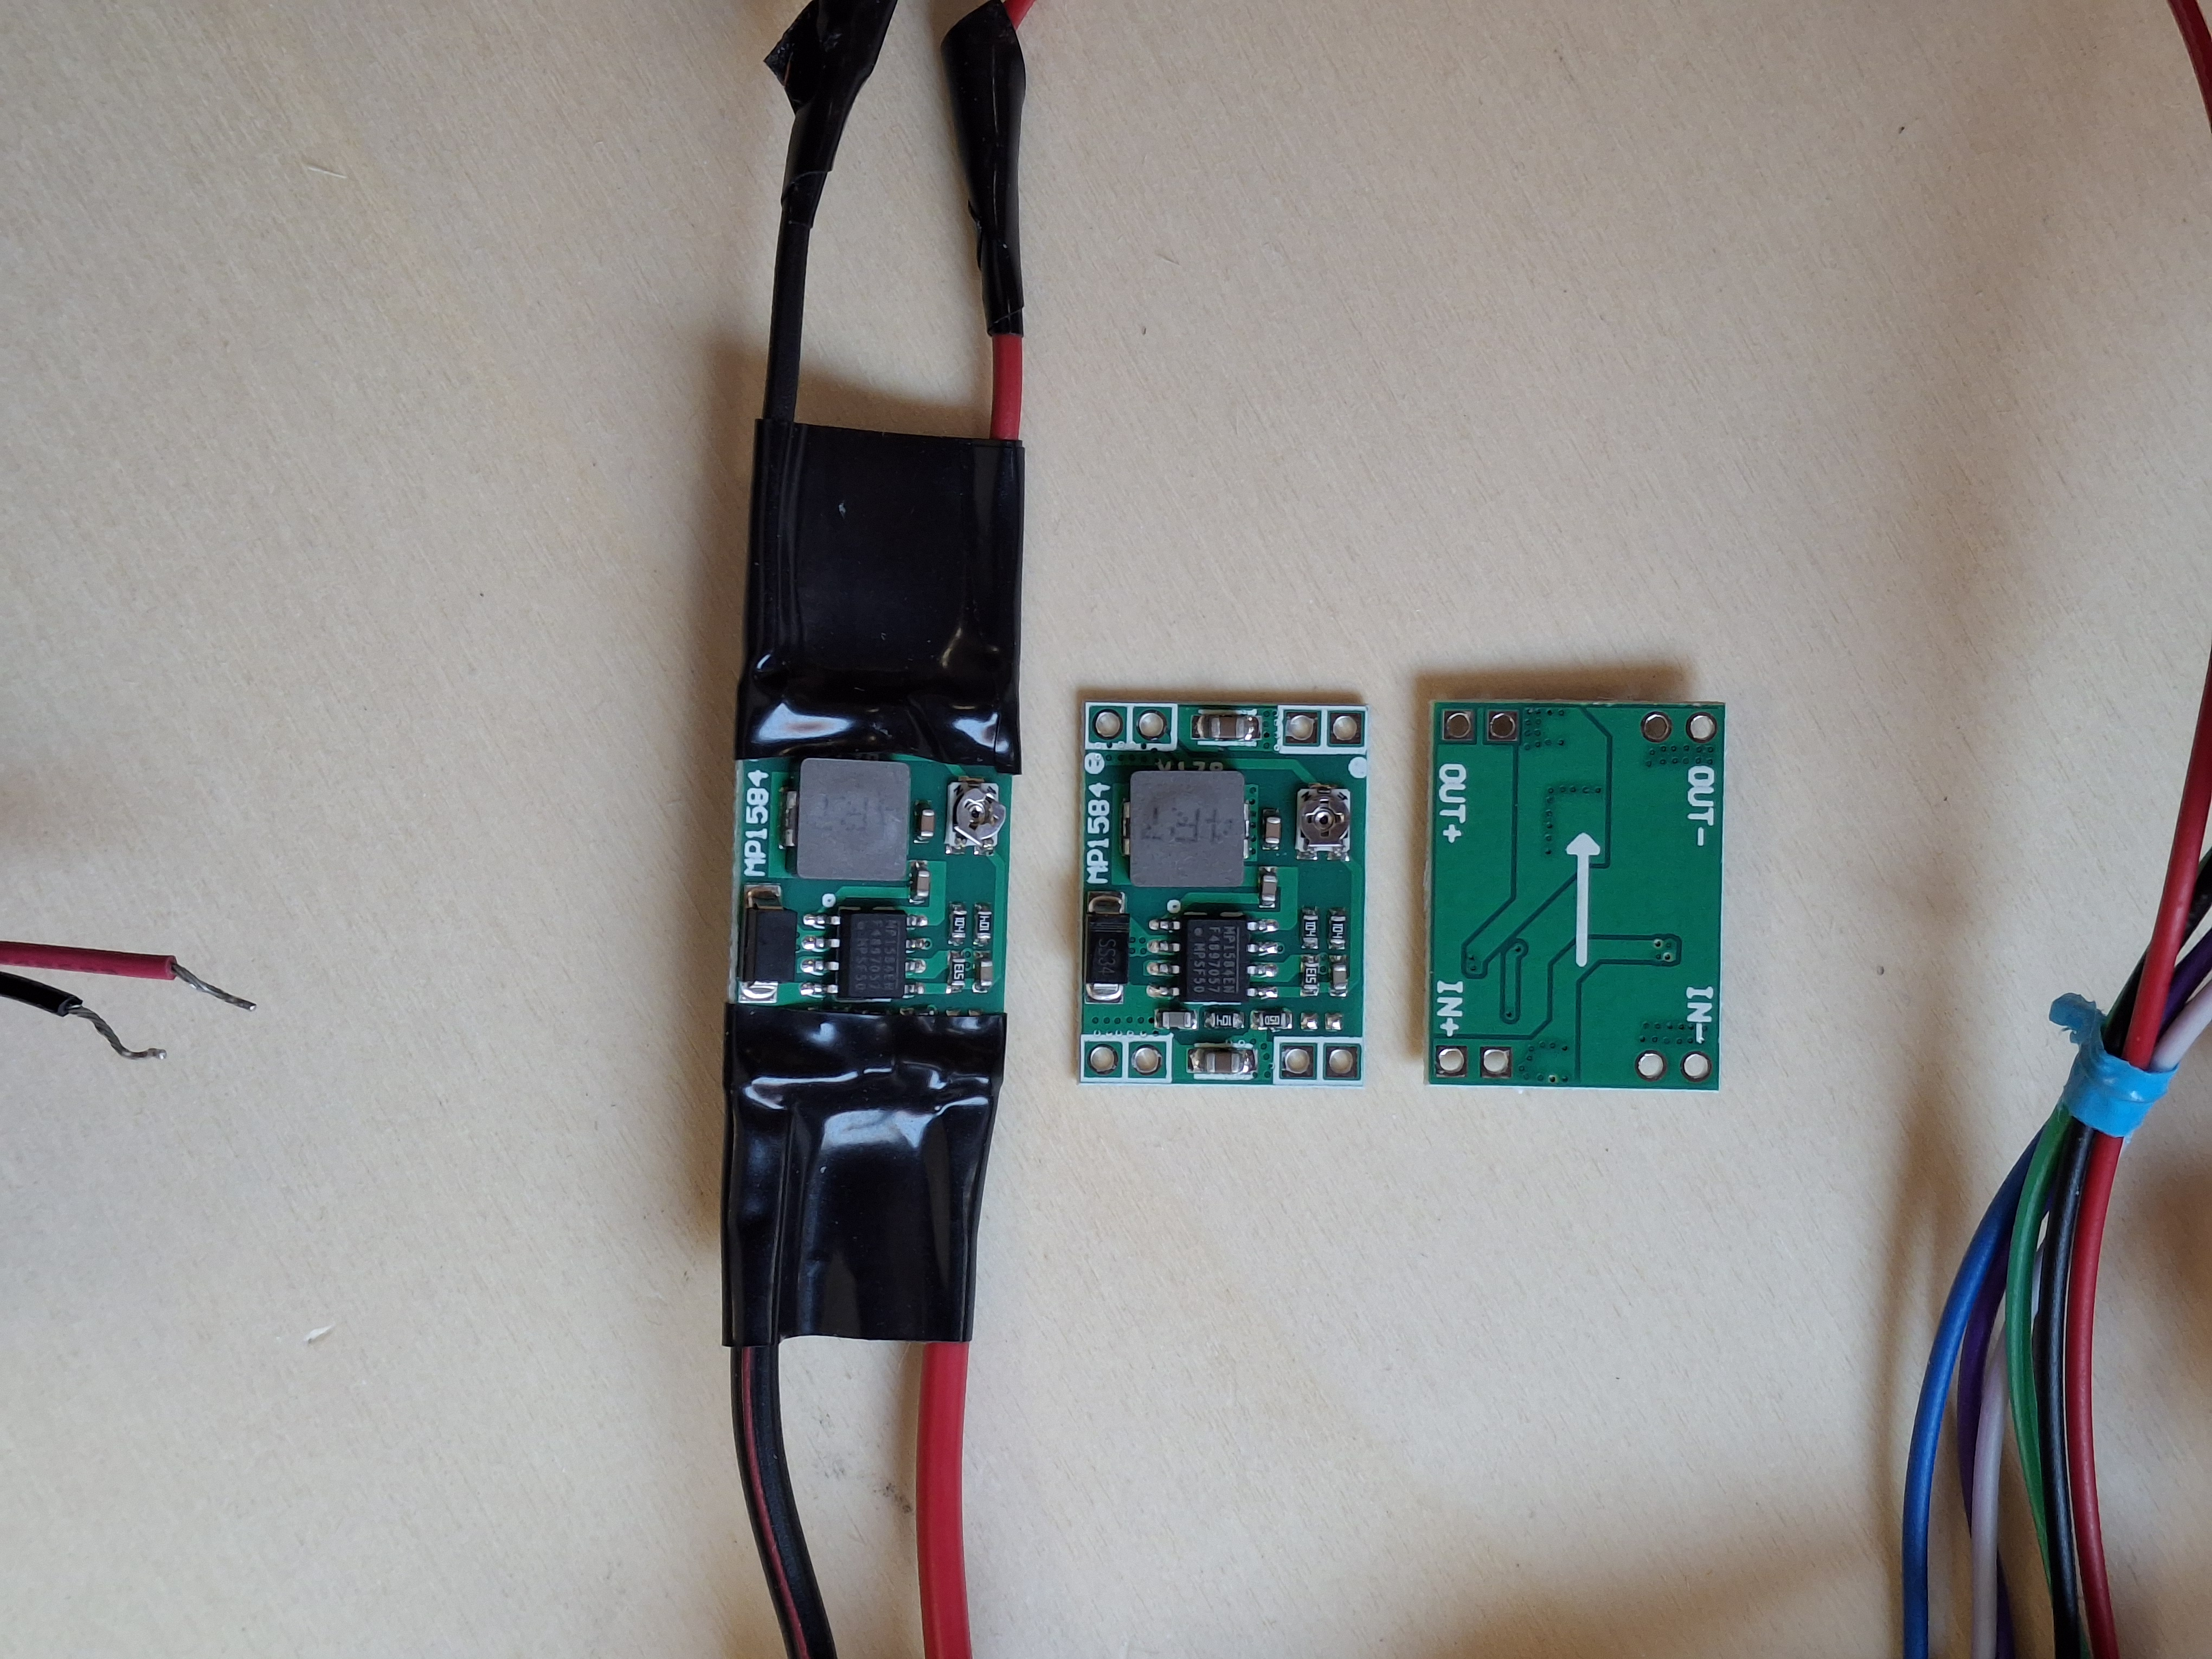
\includegraphics[width=\textwidth]{immagini/1_step_down.jpg}
        \caption{Foto dello step down per alimentare le bobine dei relè a 5 V.}
        \label{fig:step_down}
    \end{subfigure}
	\caption[Foto dei relè e dello step down]{Foto dei relè e dello step down per il controllo degi attuatori
	del prototipo di incubatrice neonatale.}
	\label{fig:rele_step_down}
\end{figure}


\subsection{Pannello frontale e sensore SHT20}
Il pannello frontale del prototipo di incubatrice neonatale fornisce l'interfaccia utente con cui l'utilizzatore può interagire
con il sistema. Si trova nella parte frontale del dispositivo ed è facilmente accessibile. Esso è composto dai seguenti
componenti:
\begin{itemize}
	\item un display LCD 20x4 con interfaccia I2C;
	\item 4 led di stato per indicare l'accensione del riscaldatore, l'accensione dell'umidificatore, la presenza di un allarme
	e la necessità di eseguire un refill del serbatoio dell'acqua dell'umidificatore;
	\item 3 switch a due posizioni per il controllo manuale del riscaldatore, dell'umidificatore e della barra led presente
	all'interno del prototipo di incubatrice neonatale;
	\item 2 potenziometri rotativi per la regolazione del setpoint di temperatura ed umidità.
\end{itemize}

\begin{figure}[htbp]
	\centering
	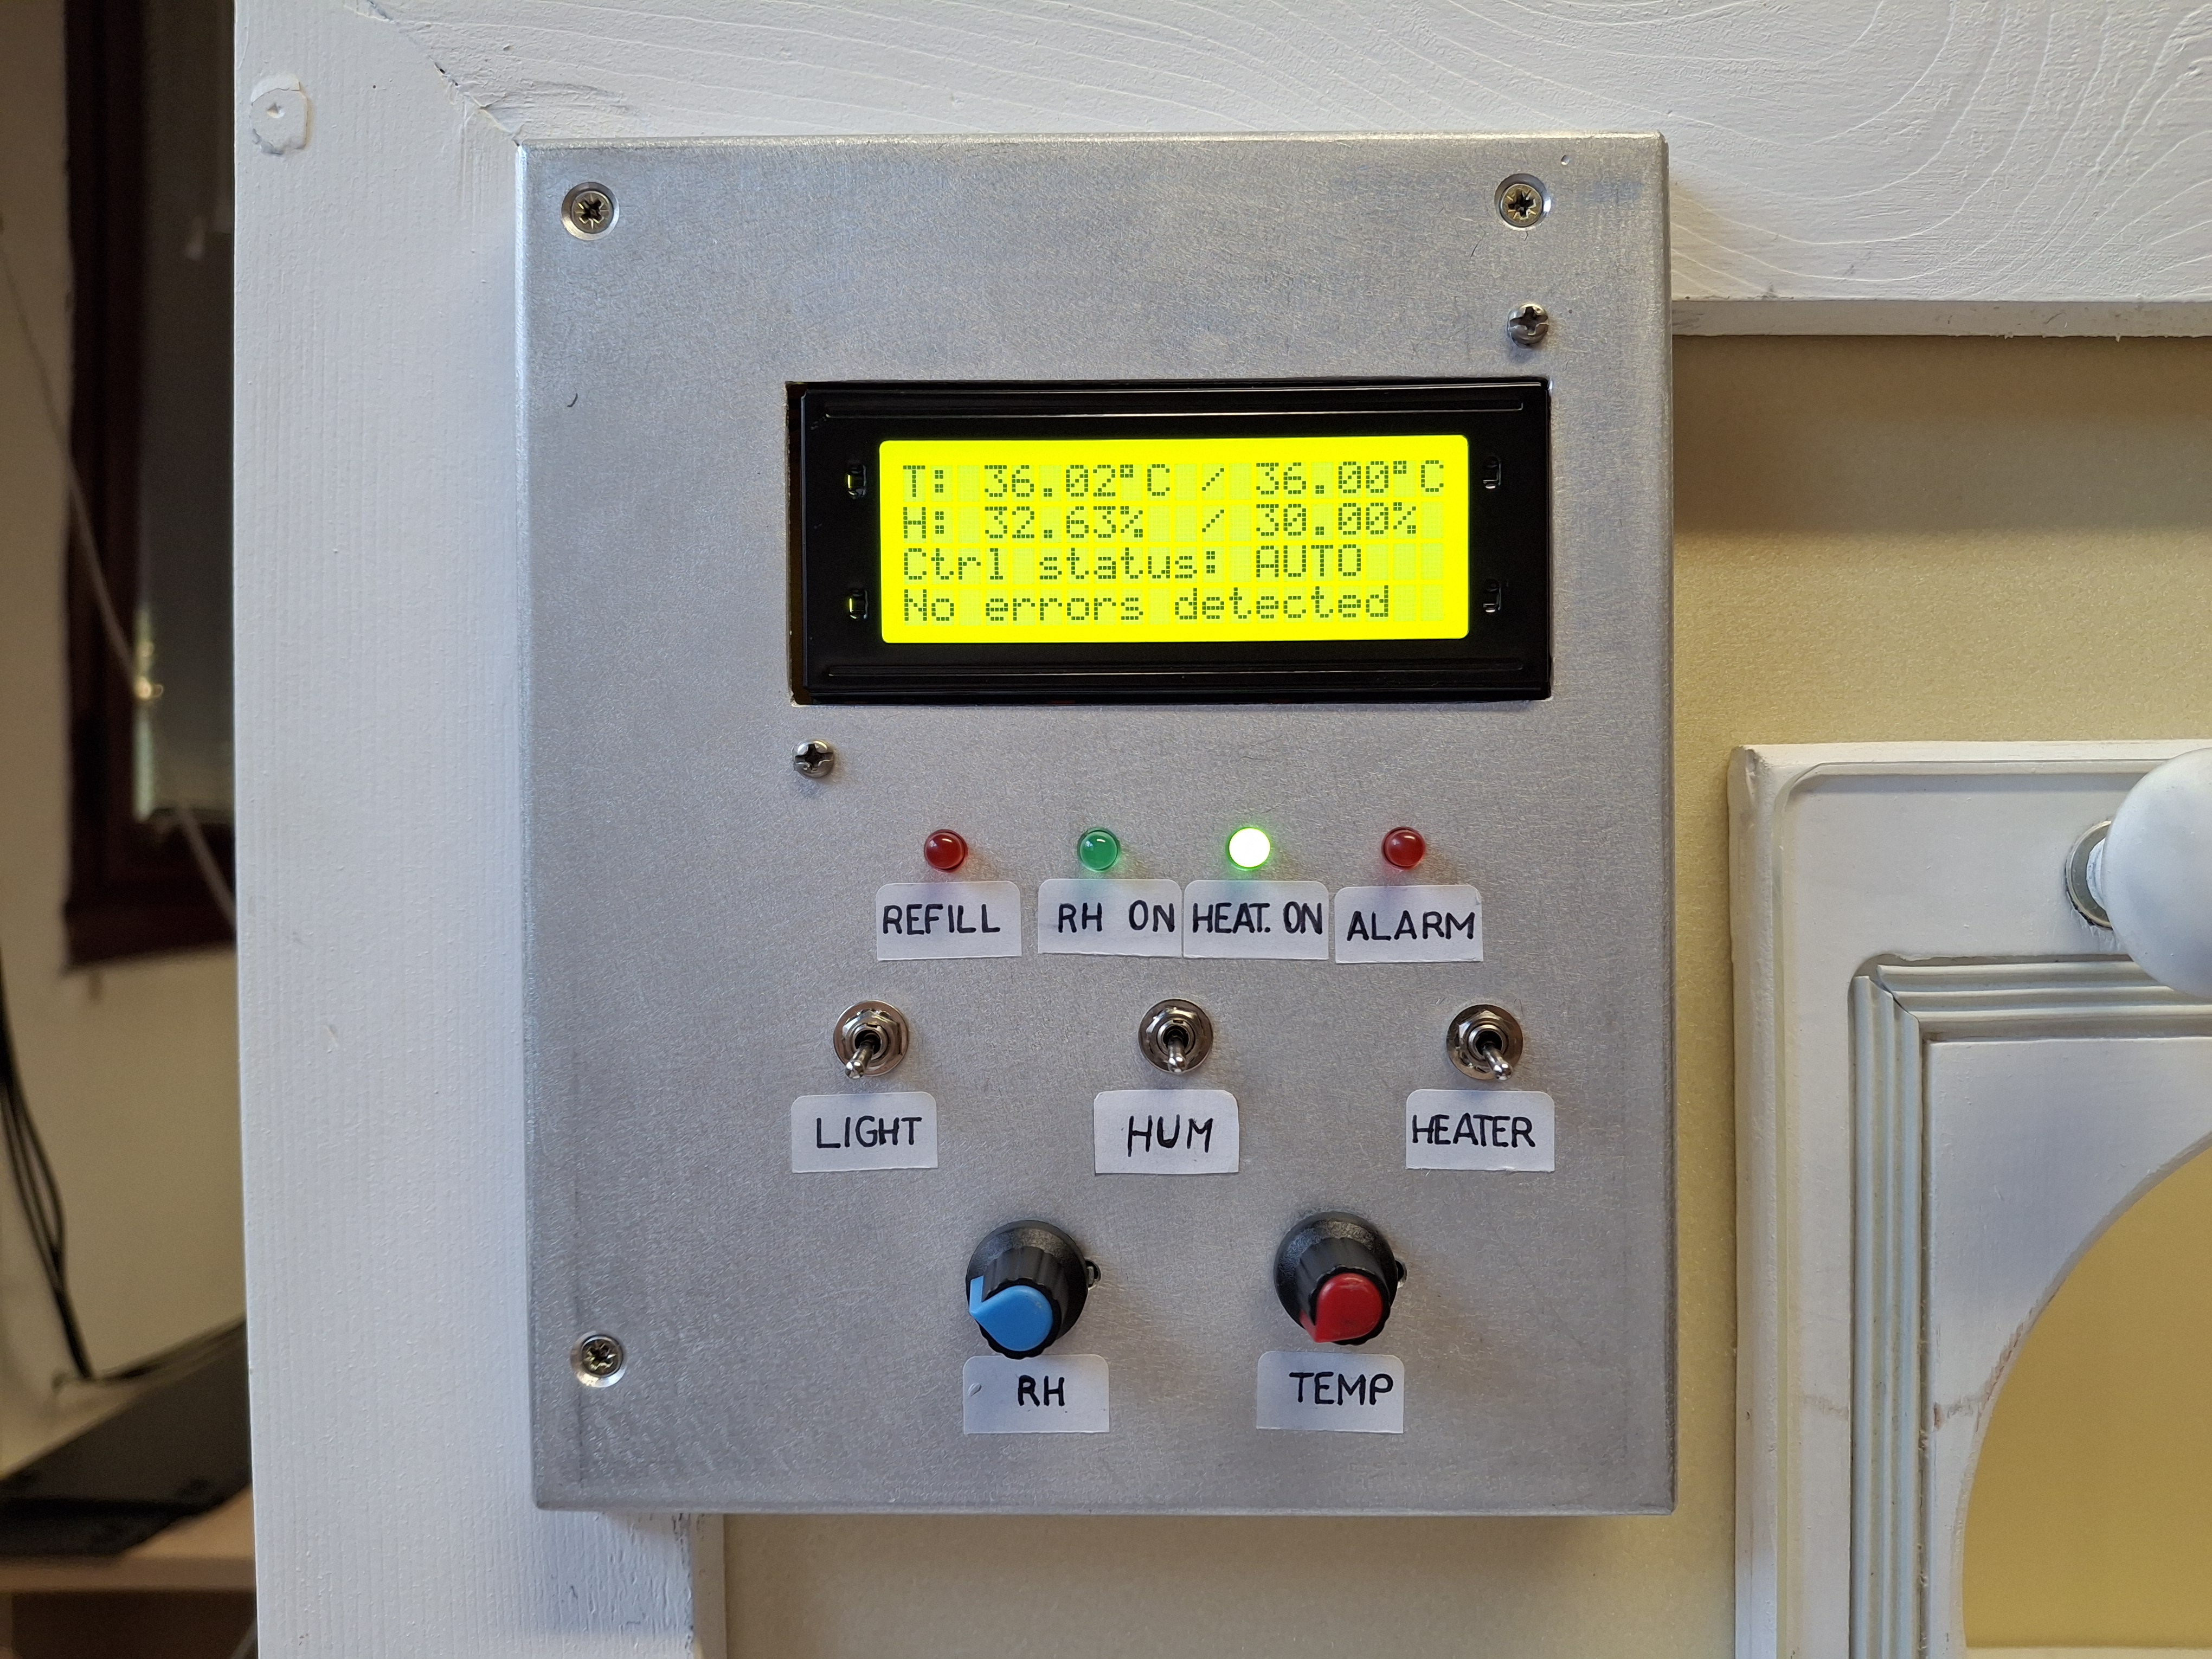
\includegraphics[width=0.9\textwidth, trim={0cm 7cm 0cm 6cm}, clip]{immagini/1_pannello_frontale_1.jpg}
	\caption[Foto del pannello frontale]{Foto del pannello frontale del prototipo di incubatrice neonatale con i vari componenti
	presenti.}
	\label{fig:pannello_frontale}
\end{figure}

Il sensore di temperatura e umidità SHT20 è un sensore digitale che permette di misurare la temperatura e l'umidità relativa
dell'ambiente in cui si trova. Esso è posizionato all'interno della camera interna del prototipo di incubatrice neonatale.
Per i test effettuati, il sensore è stato posizionato a 20 cm dalle pareti laterali lunghe, a 17 cm dalla parete corta opposta
al riscaldatore e alla ventola di omogeneizzazione dell'aria e a 7.5 cm di altezza dal piano della base della camera interna.

\begin{figure}[htbp]
	\centering
	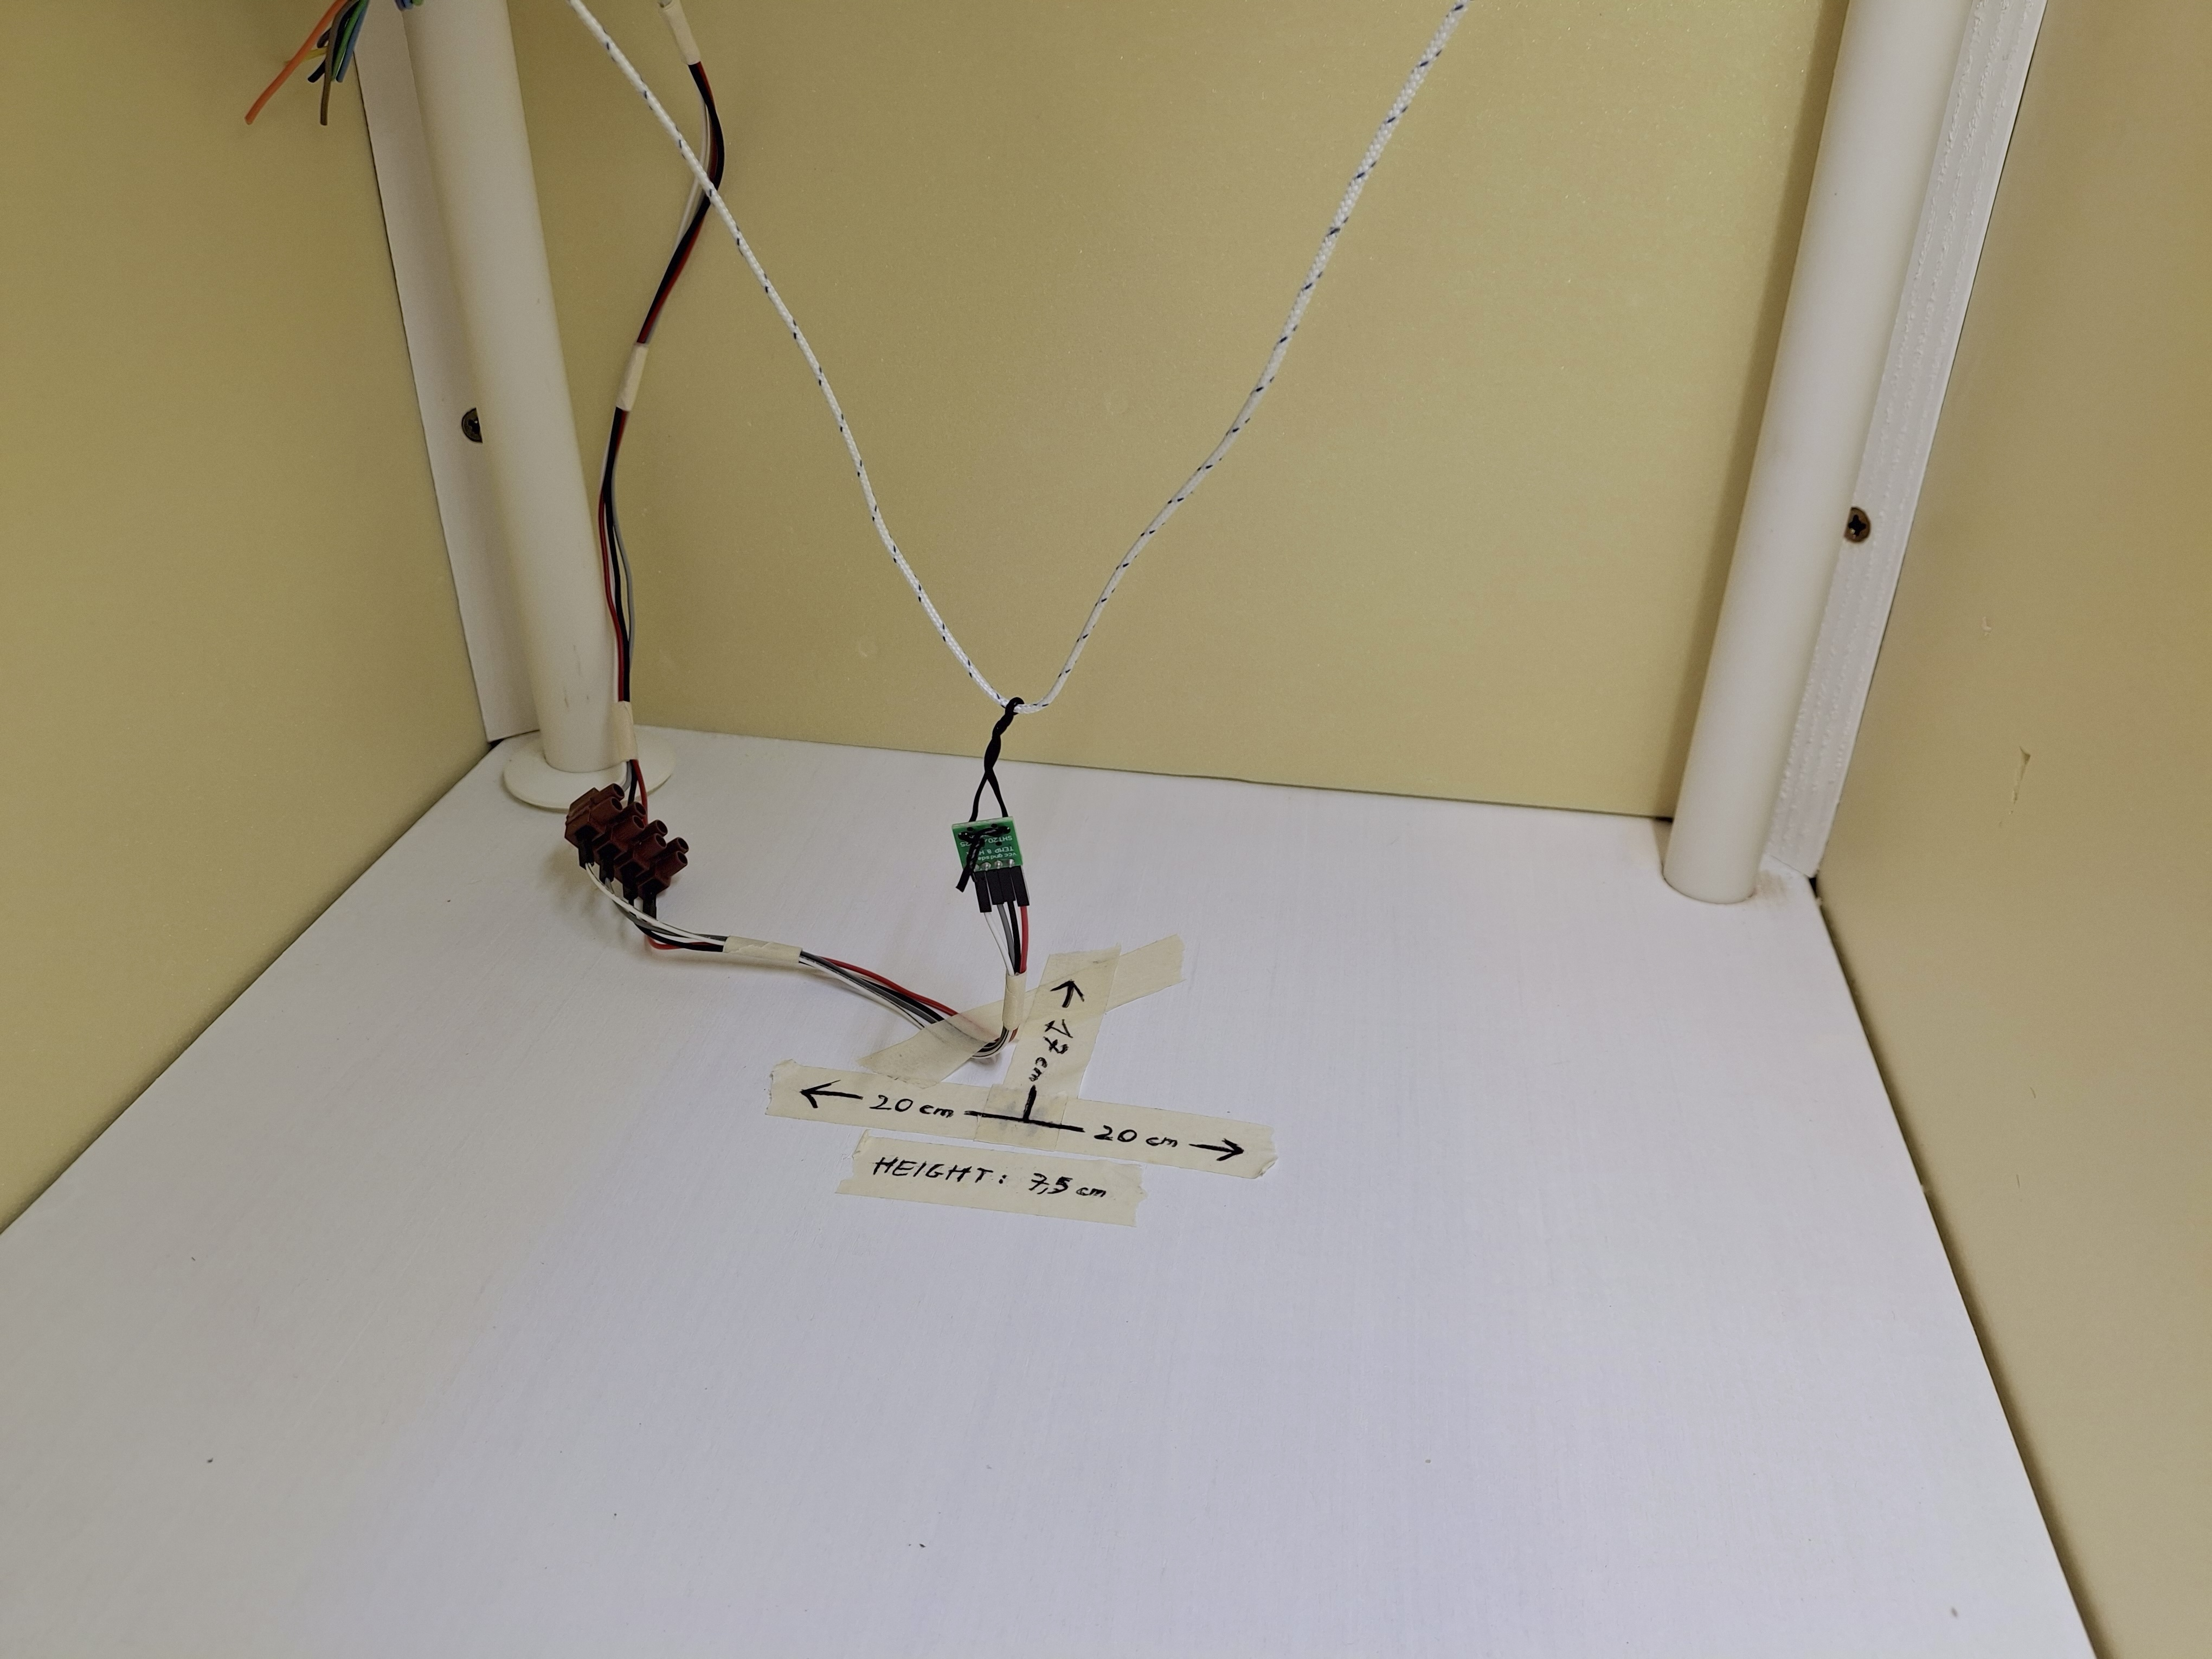
\includegraphics[width=0.9\textwidth, trim={5cm 20cm 10cm 25cm}, clip]{immagini/1_sht20.jpg}
	\caption[Foto del sensore SHT20]{Sensore di temperatura e umidità SHT20 posizionato all'interno della camera interna del
	prototipo di incubatrice neonatale.}
	\label{fig:sht20}
\end{figure}


\subsection{Scheda Arduino Mega 2560}
Per gestire i vari componenti elettronici del prototipo di incubatrice neonatale, è stata utilizzata una scheda Arduino Mega 2560
con microcontrollore ATmega2560. Essa è stata scelta per la sua semplicità d'uso, la disponibilità di numerosi pin di input/output
e l'elevato spazio di memoria disponibile per il firmware. La scheda è posizionata all'interno del cassetto inferiore del prototipo
di incubatrice neonatale, insieme a tutti i cablaggi provenienti dai vari componenti elettronici. La scheda è alimentata via USB
da un computer esterno su cui è possibile visualizzare i dati provenienti dal microcontrollore.

\begin{figure}[htbp]
	\centering
	%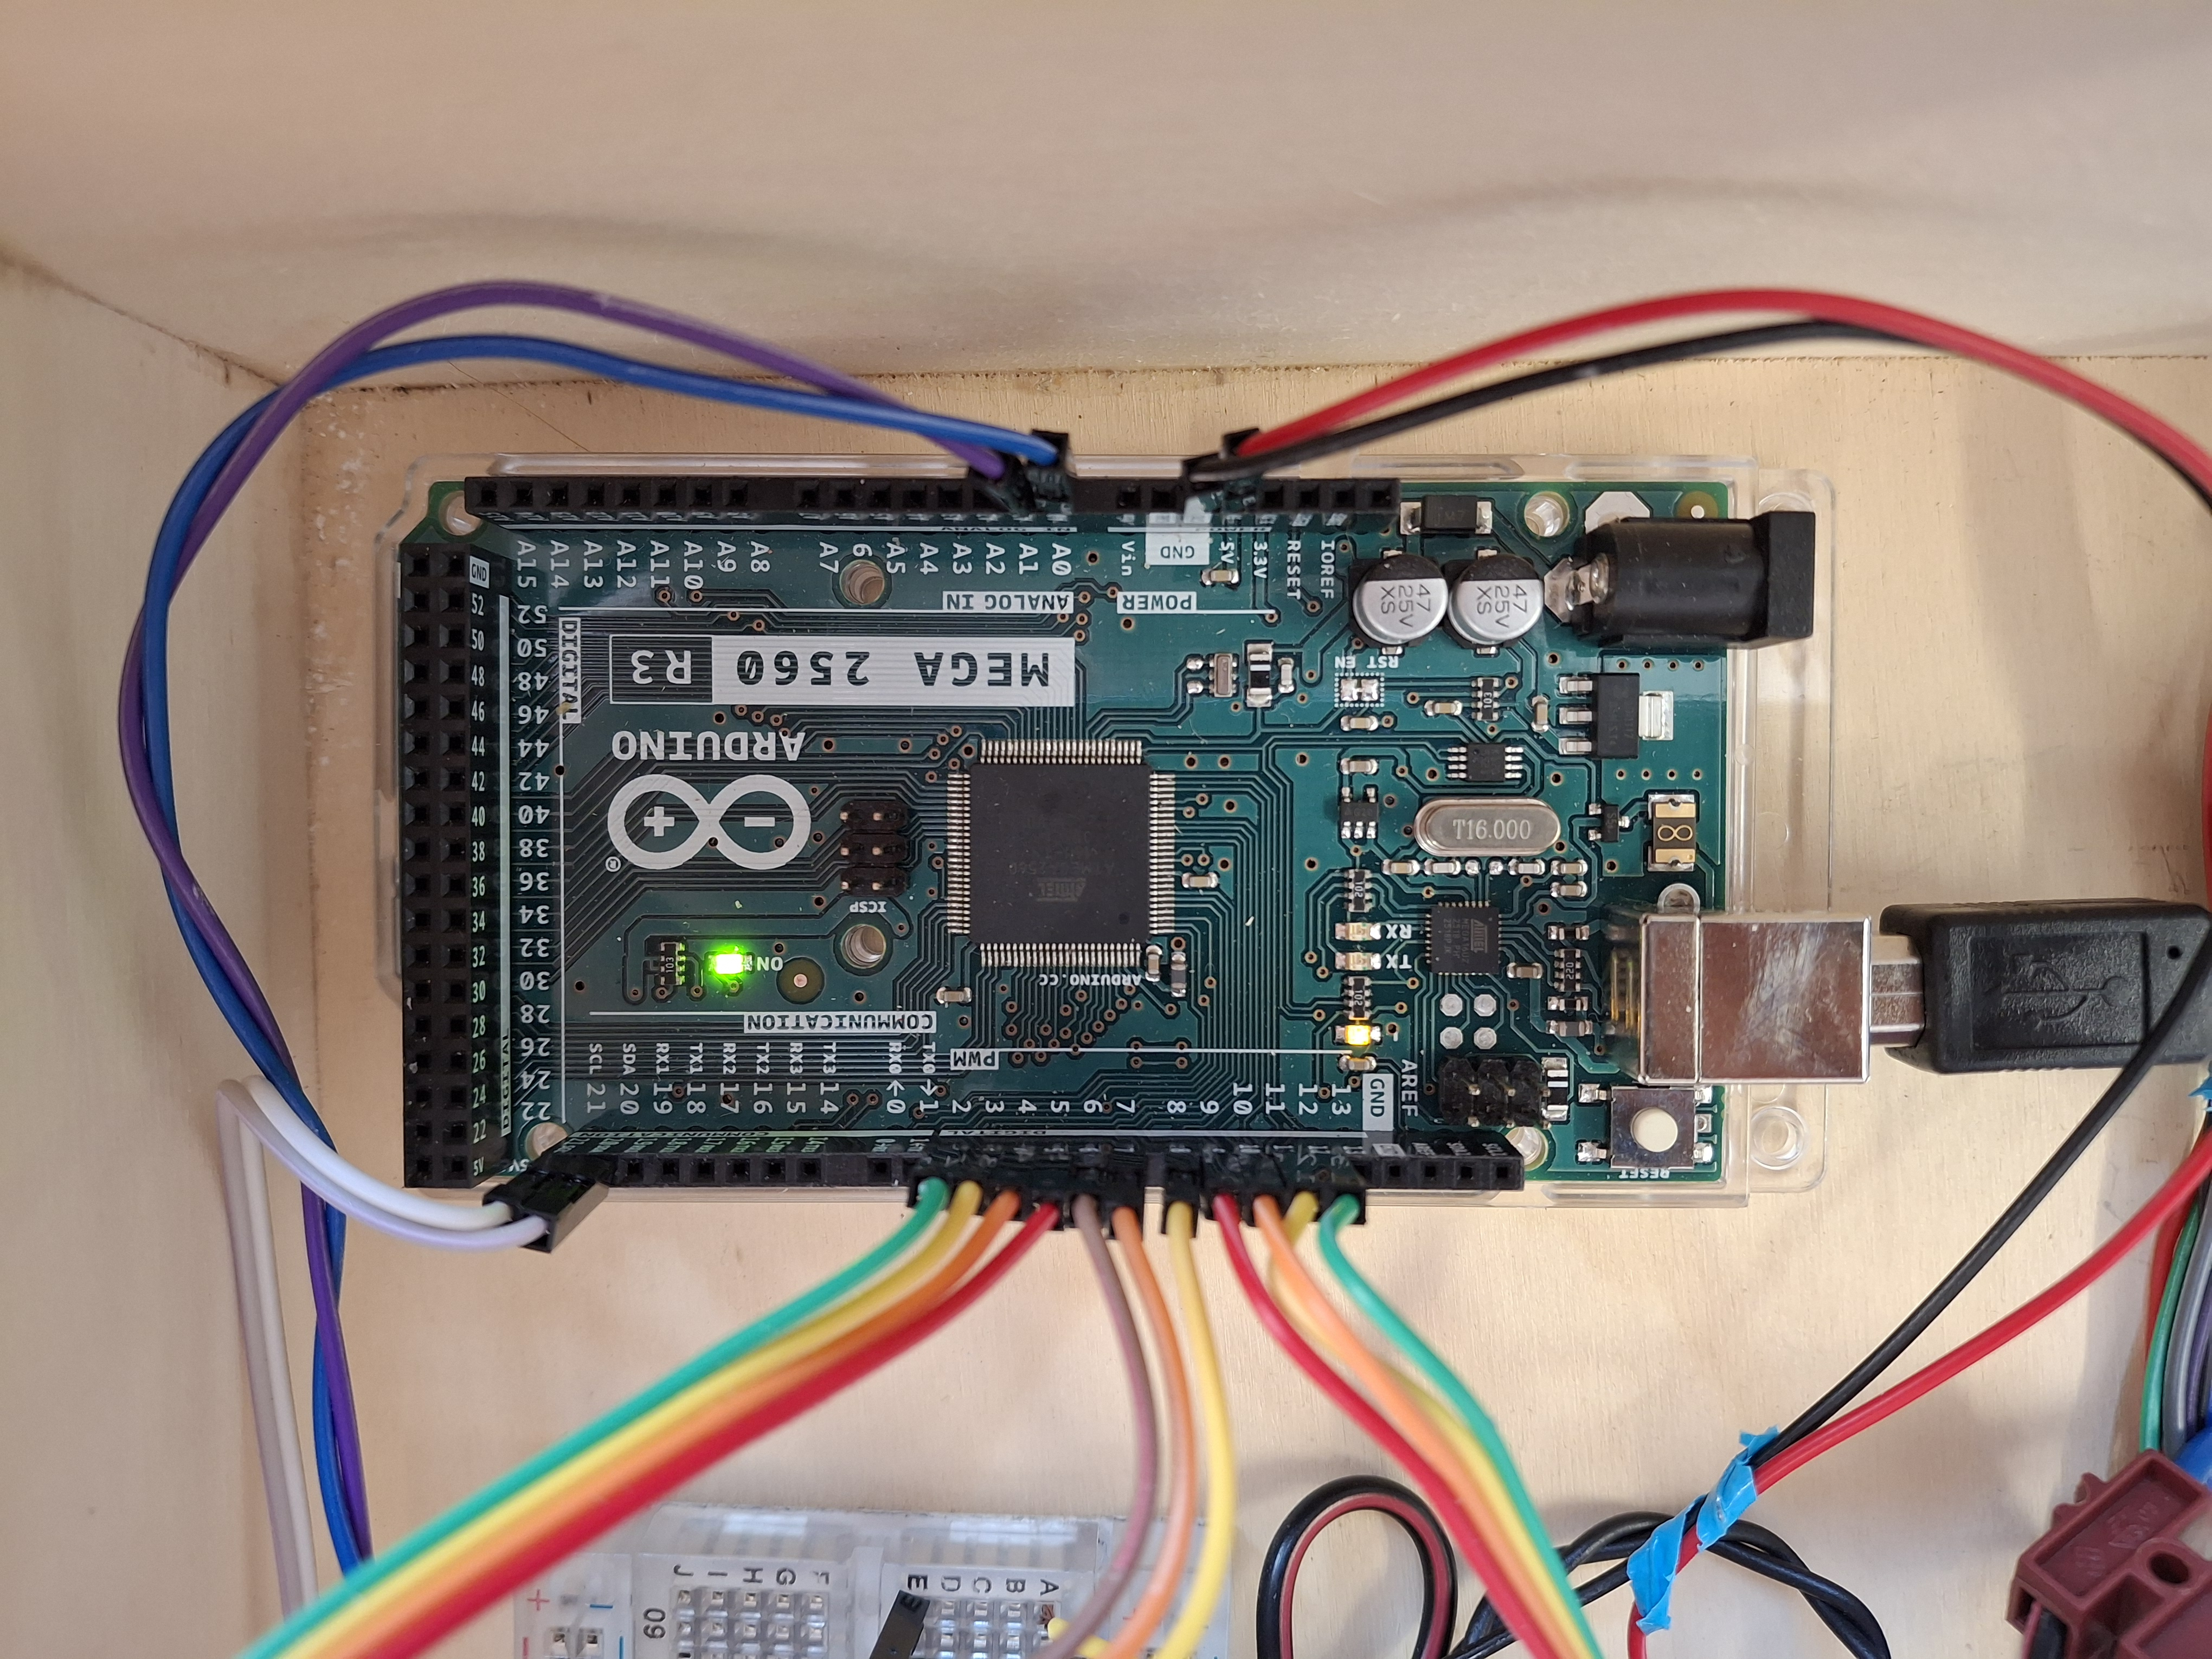
\includegraphics[width=0.9\textwidth]{immagini/1_arduino_mega.jpg}
	\caption[Foto della scheda Arduino Mega 2560]{Scheda Arduino Mega 2560 posizionata all'interno del cassetto inferiore del
	prototipo di incubatrice neonatale.}
	\label{fig:arduino_mega}
\end{figure}


\section{Collegamento delle periferiche al microcontrollore}
\subsection{Connessioni dei relè ai diversi attuatori}
Di seguito è riportato lo schema elettrico con le connessioni tra i relè e i vari attuatori presenti nel prototipo di incubatrice
neonatale realizzato con il software Fritzing. Sono indicati anche i cavi di collegamento tra i relè e la scheda Arduino, insieme
al convertitore step down per alimentare le bobine dei relè a 5 V.

Si evidenzia come l'umidificatore disponga di un suo sistema di alimentazione separato a 24 V, evidenziato dalla presenza del
tratteggio sui cavi rosso e nero. Inoltre si nota che la massa dello step down e quella dei relè non sono immediatamente collegate
tra di loro perché per distribuire la massa si utilizza la topologia a stella. Questo significa che tutti i componenti elettronici
sono collegati a un unico punto di massa (mostrato nello schema dell'Arduino), eliminando i problemi di ground lifting e riducendo
al minimo le interferenze dovute a sbalzi di corrente in corrispondenza delle commutazioni dei relè.

\begin{figure}[htbp]
	\centering
	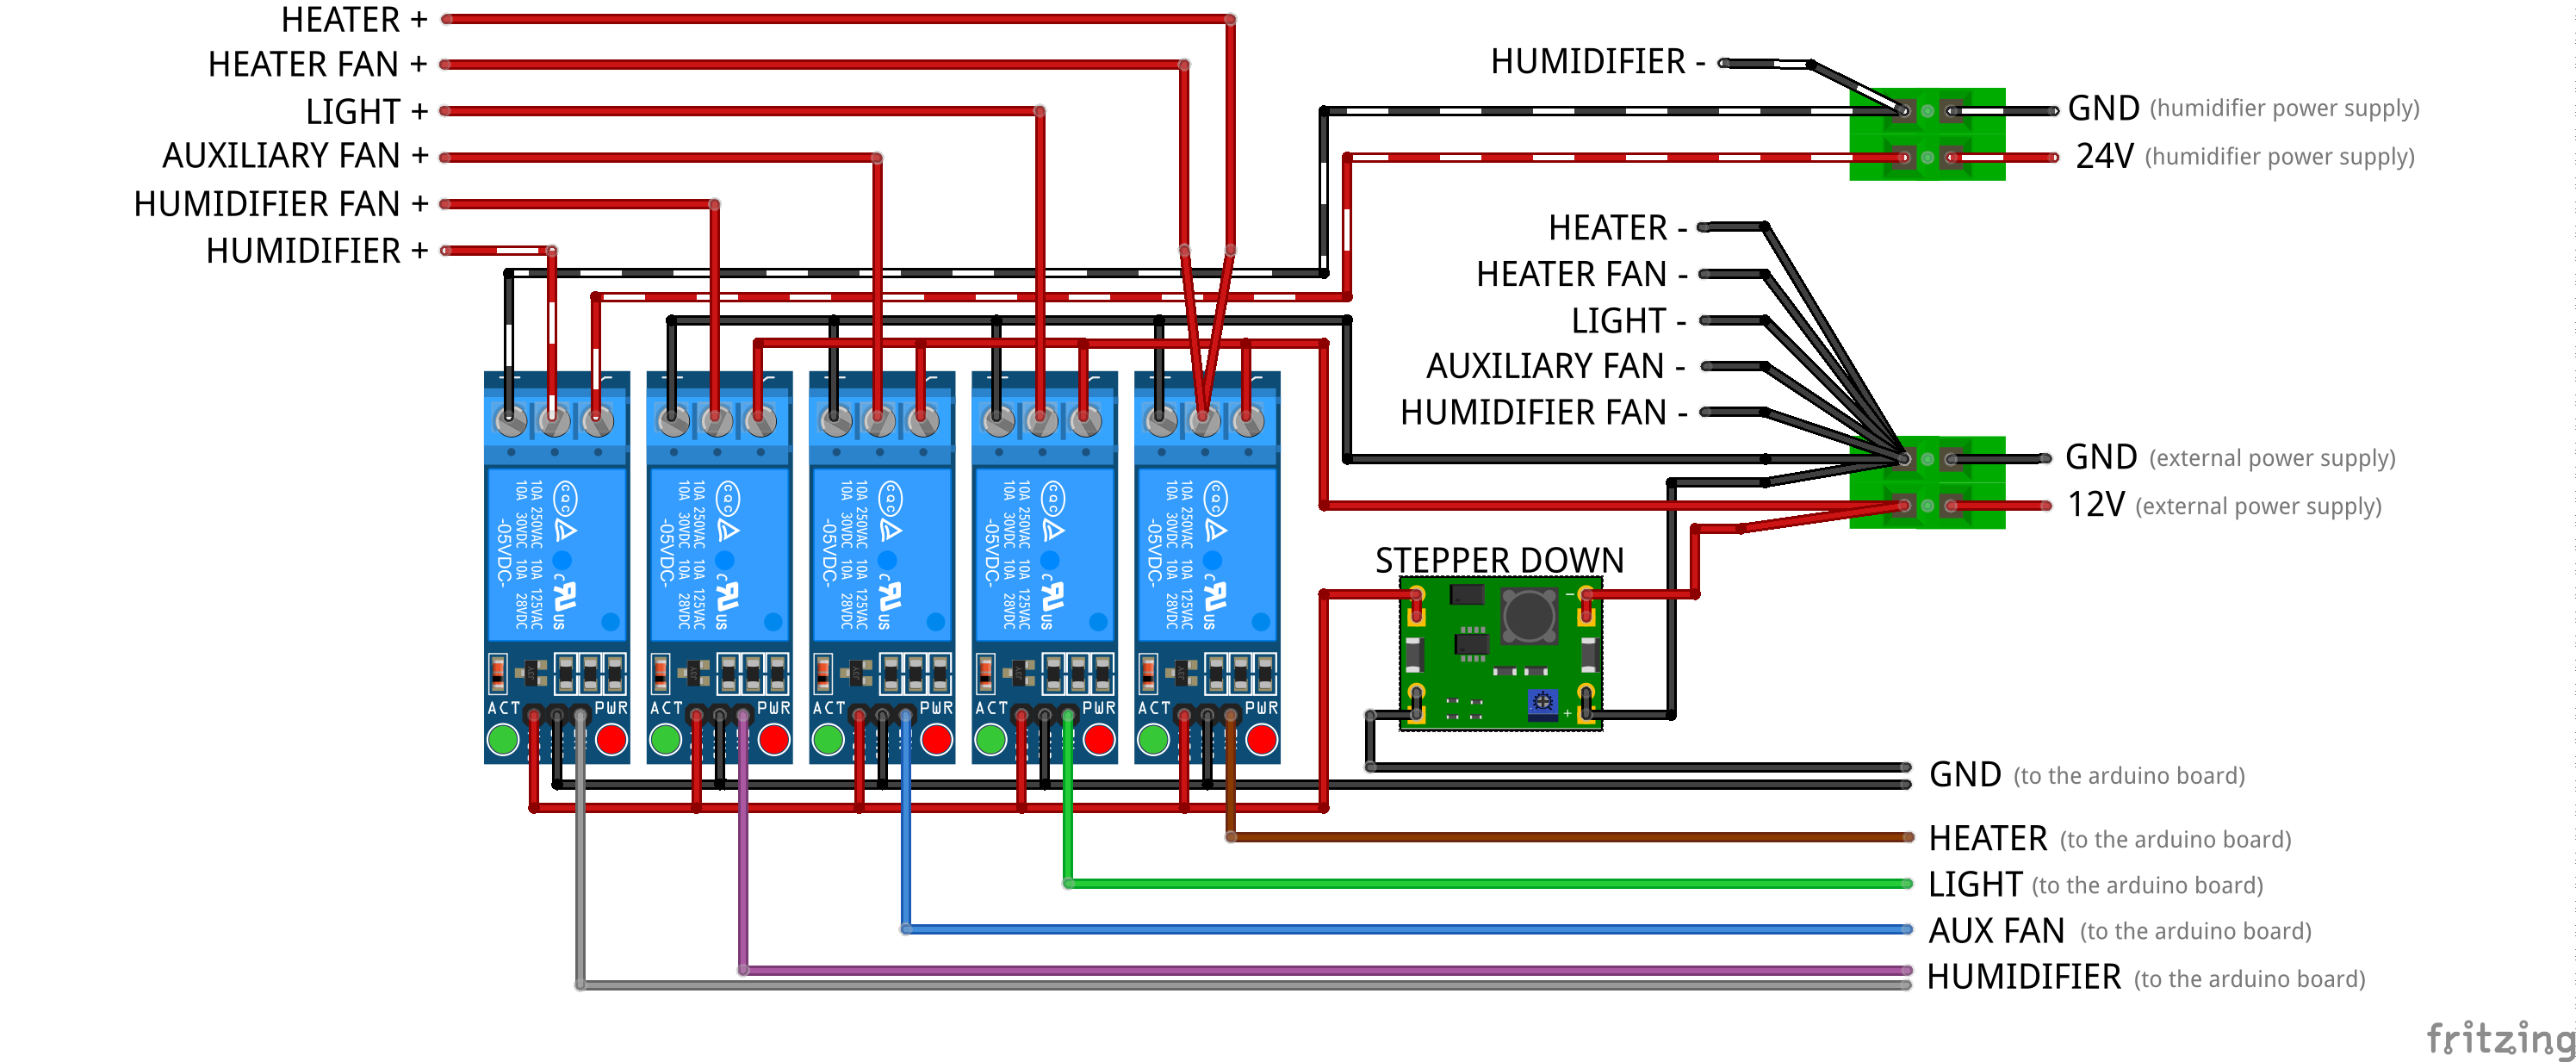
\includegraphics[width=0.9\textwidth]{immagini/1_circuito_1.png}
	\caption[Schema circuitale dei relè e degli attuatori]{Schema elettrico con le connessioni dei relè e degli attuatori
	presenti nel prototipo di incubatrice neonatale.}
	\label{fig:circuito_1}
\end{figure}

%\begin{figure}[htbp]
%	\centering
%	\includegraphics[width=0.9\textwidth]{immagini/1_foto_circuito_1.png}
%	\caption[Foto delle connessioni tra relè e attuatori]{Foto delle connessioni tra i relè e gli attuatori presenti nel
%	prototipo di incubatrice neonatale.}
%	\label{fig:foto_circuito_1}
%\end{figure}

\subsection{Connessioni del pannello frontale e del sensore SHT20}
I componenti del pannello frontale e il sensore SHT20 sono collegati al microcontrollore tramite due cavi multipolari da 10
conduttori ciascuno. Il cablaggio è alloggiato in una canalina dedicata che unisce il cassetto inferiore al pannello frontale
e alla camera interna dell'incubatrice.

Al fine di garantire affidabilità e agevolare le future operazioni di manutenzione, le connessioni verso il pannello frontale
sono state modularizzate utilizzando dei connettori JST disponibili in laboratorio. In particolare sono stati scelti tre connettori
a 4 pin per i segnali di controllo e un connettore a 2 pin per l'alimentazione. Le connessioni interne tra i componenti del pannello
frontale, la catena di alimentazione e i rispettivi connettori sono state saldate con stagno per garantire un collegamento stabile
e duraturo nel tempo.

Il sensore SHT20, per mantenere una certa flessibilità nella sua posizione all'interno della camera interna, è stato collegato
ai cavi della canalina tramite una serie di 4 morsetti mammuth. In questo modo è possibile scollegare il sensore, allungare o
accorciare i cavi per poter posizionare agevolmente il sensore in diverse posizioni.

Per maggiore leggibilità, è stato scelto di tratteggiare i conduttori del cavo multipolare che collega il sensore SHT20 e il
led di refill al microcontrollore. Si nota che non tutti i conduttori di questo cavo sono stati utilizzati.

\begin{figure}[htbp]
    \centering
    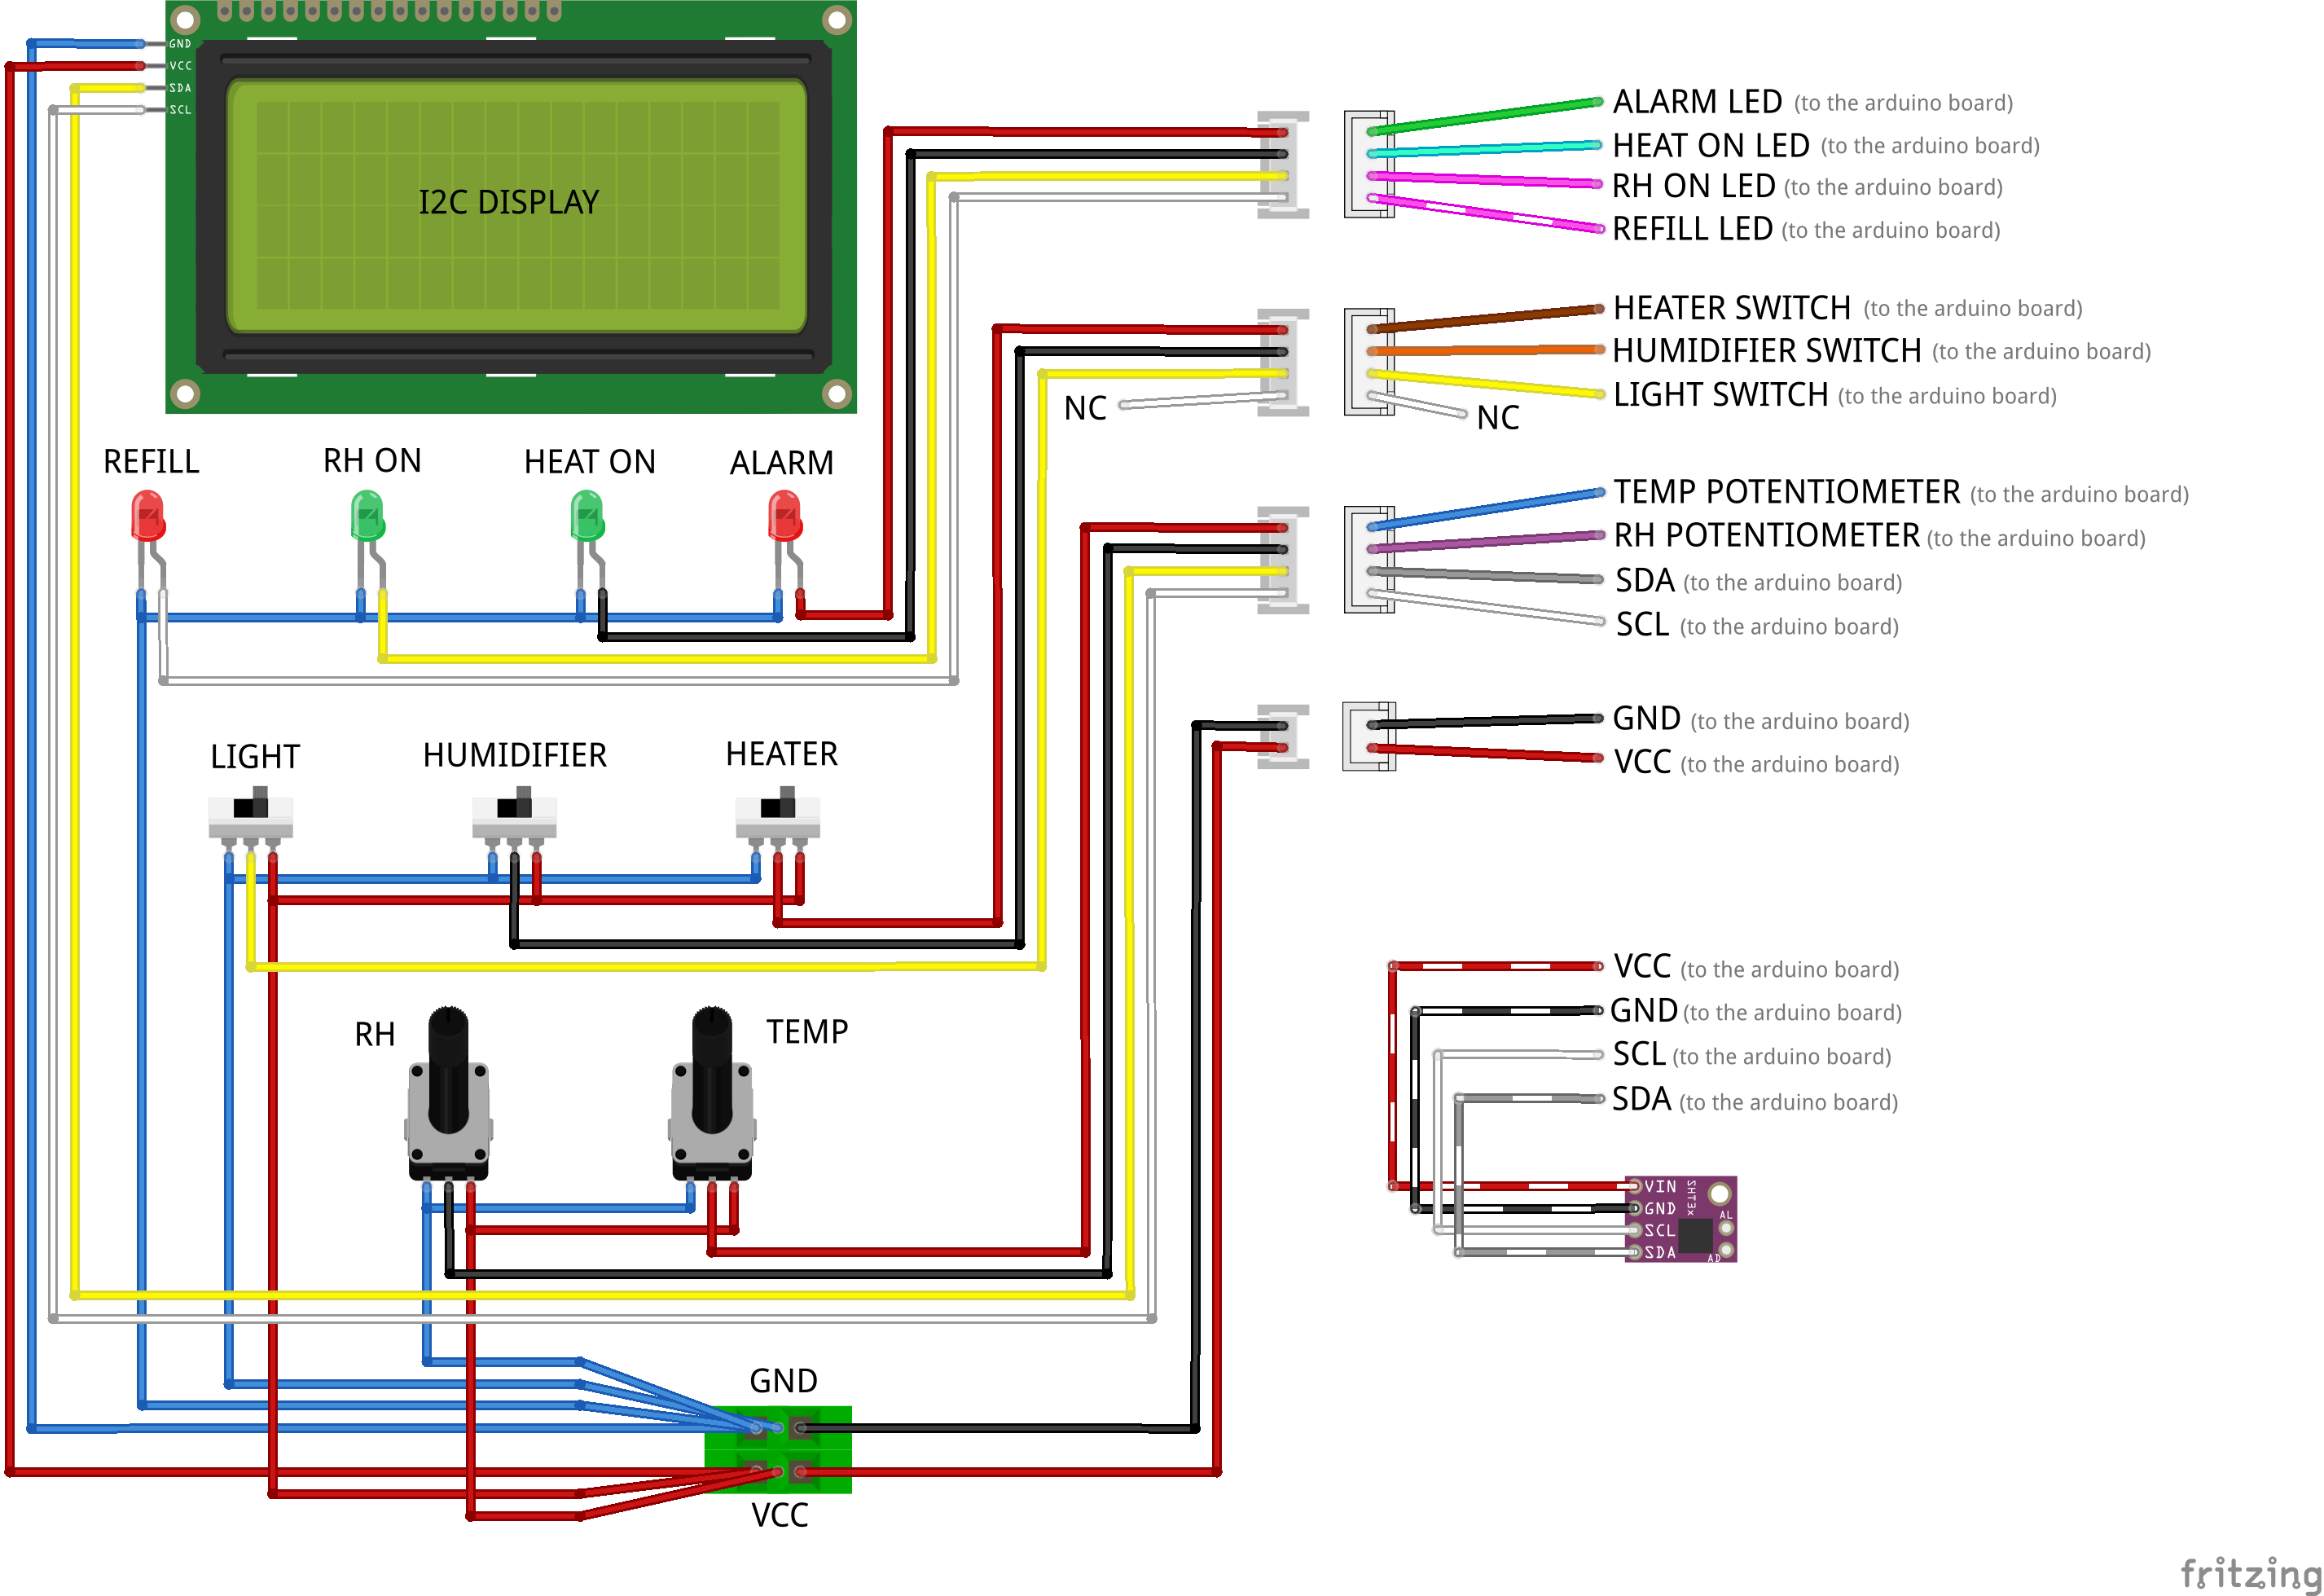
\includegraphics[width=0.9\textwidth]{immagini/1_circuito_2.png}
    \caption[Schema circuitale del pannello frontale e del sensore SHT20]{Schema elettrico con le connessioni del sensore di
	temperatura e umidità SHT20 e dei vari componenti presenti nel pannello frontale del prototipo di incubatrice neonatale.}
    \label{fig:circuito_2}
\end{figure}

%\begin{figure}[htbp]
%    \centering
%    \includegraphics[width=0.9\textwidth]{immagini/1_foto_circuito_2.png}
%    \caption[Foto delle connessioni nel pannello frontale]{Foto delle connessioni tra i vari componenti presenti nel pannello
%	frontale del prototipo di incubatrice neonatale.}
%    \label{fig:foto_circuito_2}
%\end{figure}

\subsection{Connessioni dei vari componenti al microcontrollore}
Nel seguente schema elettrico sono riportate tutte le connessioni tra i cavi multipolari provenienti dai vari componenti
del prototipo e i cavi di controllo dei relè con i pin del microcontrollore. Si nota la presenza del nodo principale di massa
a cui convergono tutti i cavi di massa dei vari componenti.

Per limitare la corrente nei led di stato del pannello frontale, sono state inserite delle resistenze di bias. I relativi valori
sono stati calcolati in modo da garantire una corrente di circa 10 mA e sono poi state aggiustate in maniera empirica per ottenere
una luminosità dei led adeguata. Di seguito sono riportati i valori e le misurazioni effettive della corrente nei led di stato.
Si nota come le resistenze dei led di colore rosso siano più alte rispetto a quelle dei led di colore verde, in quanto, a parità
di corrente, i led rossi risultano più luminosi rispetto a quelli verdi.

\begin{table}[htbp]
	\centering
	\begin{tabular}{c | c | c}
		\textbf{Led} & \textbf{Resistenza} & \textbf{Corrente} \\
		\toprule
		Allarme (rosso) & 470 $\Omega$ & 6.10 mA \\
		\midrule
		Riscaldatore (verde) & 220 $\Omega$ & 12.2 mA \\
		\midrule
		Umidificatore (verde) & 220 $\Omega$ & 12.2 mA \\
		\midrule
		Refill (rosso) & 470 $\Omega$ & 6.11 mA
	\end{tabular}
	\caption{Valori e misurazioni della corrente nei led di stato}
	\label{tab:led_current}
\end{table}

\begin{figure}[htbp]
    \centering
    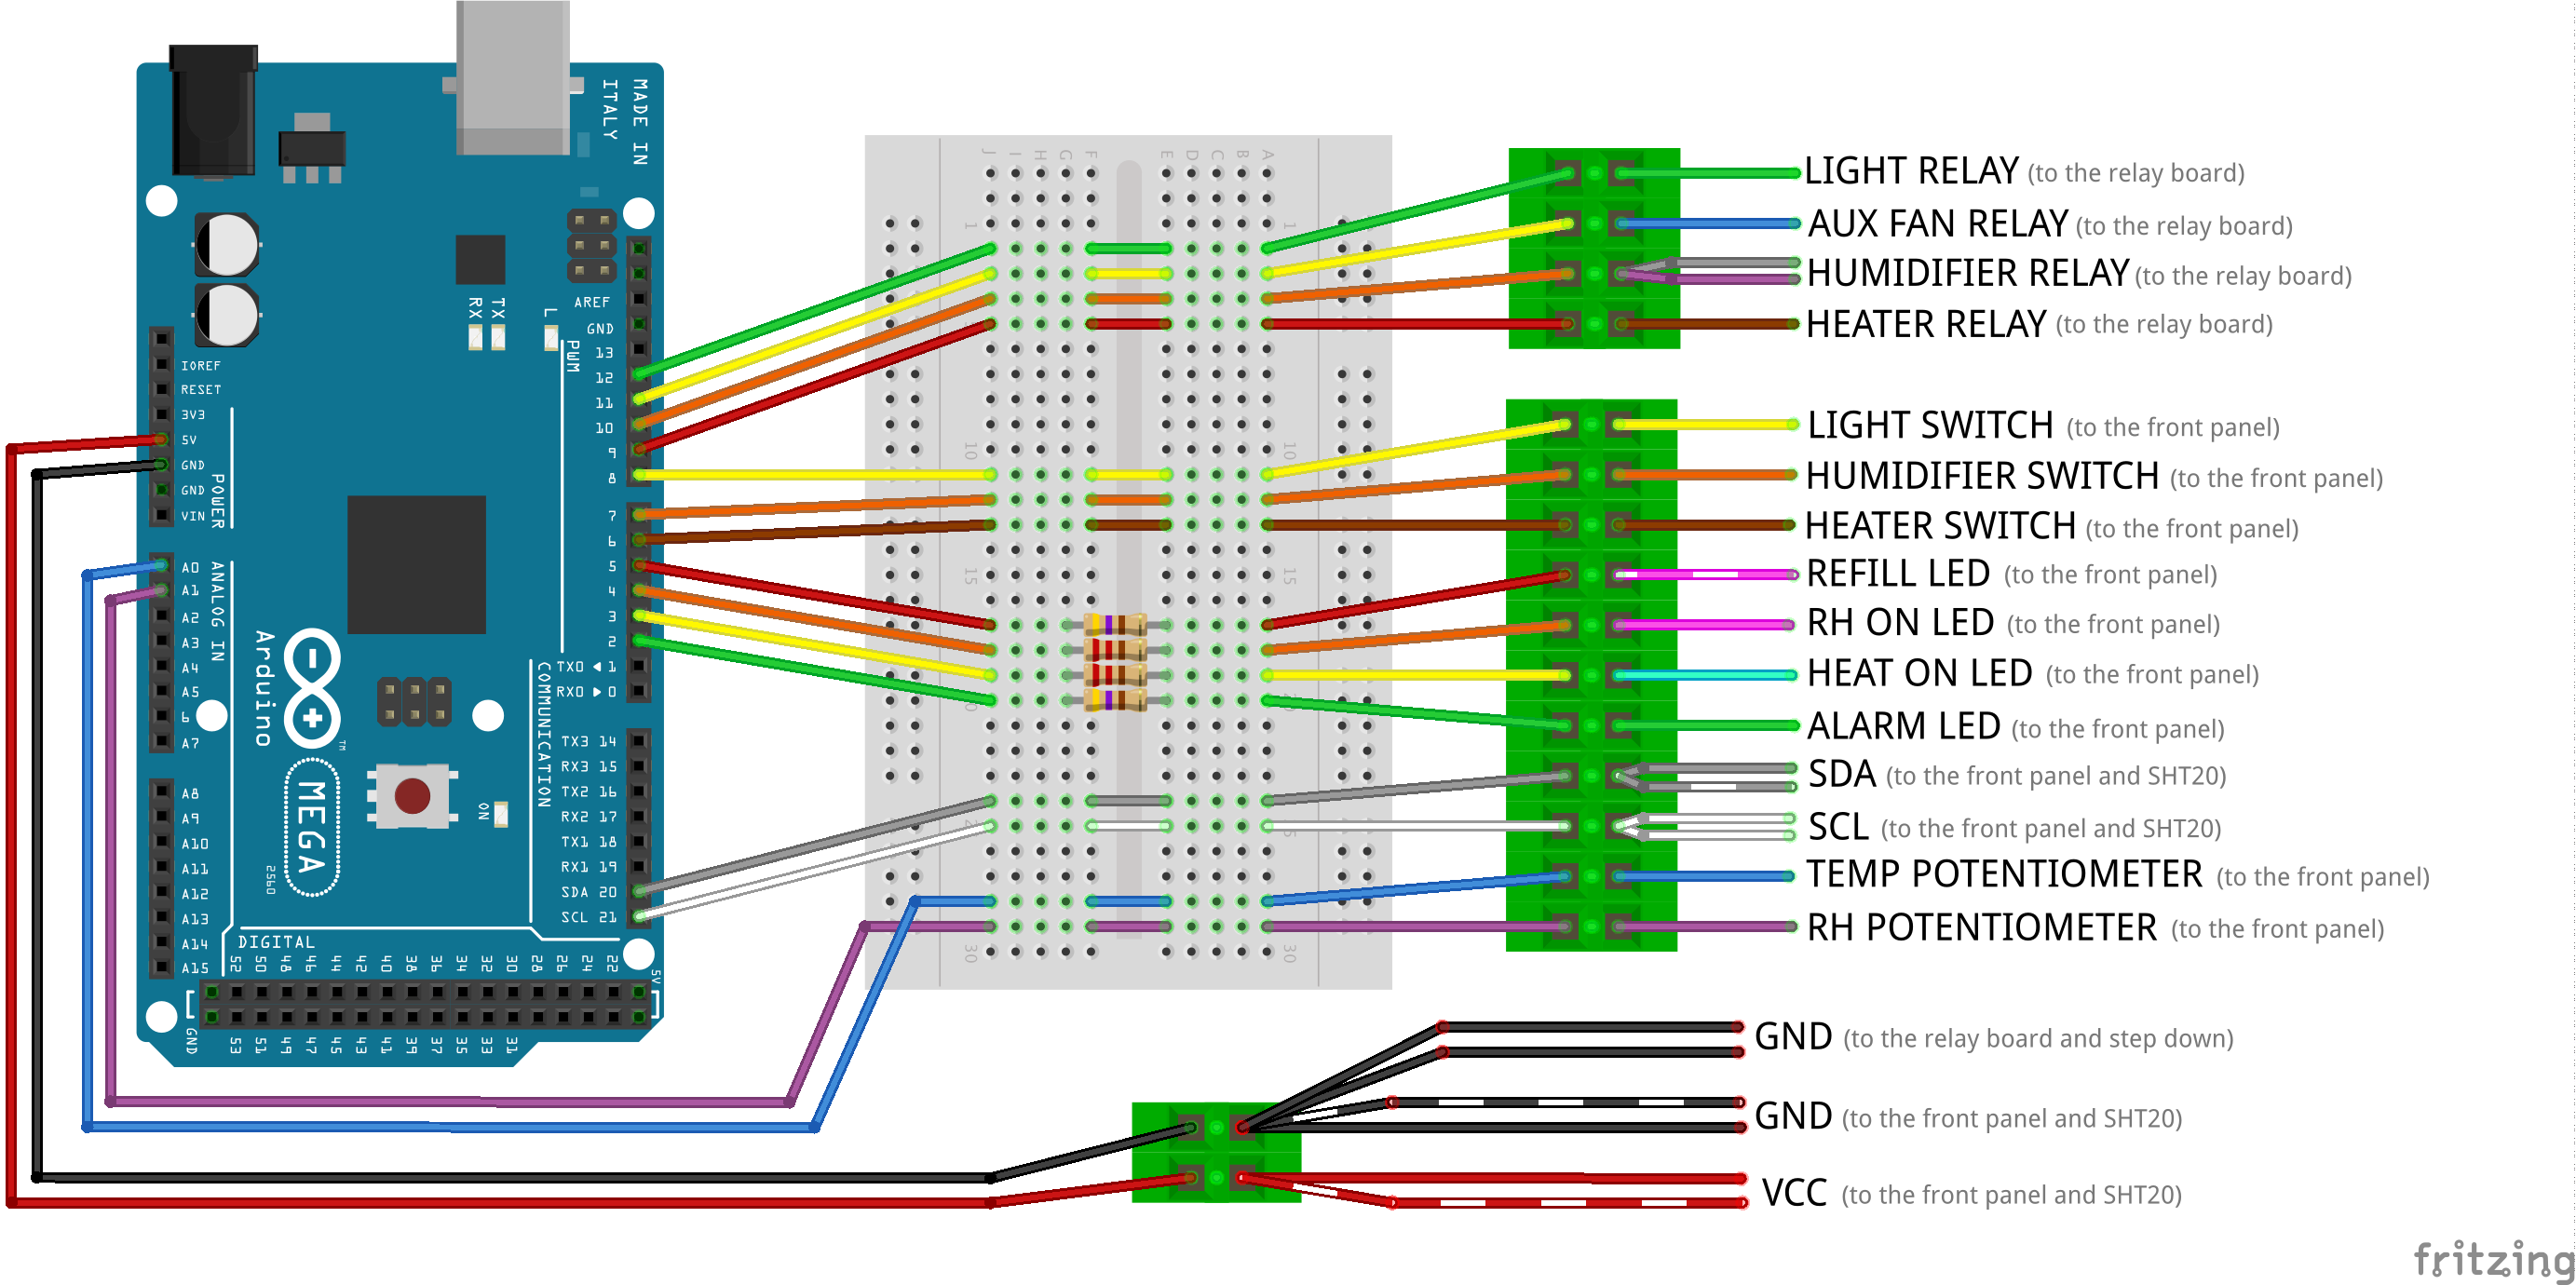
\includegraphics[width=0.9\textwidth]{immagini/1_circuito_3.png}
    \caption[Schema circuitale del microcontrollore]{Schema elettrico con le connessioni dei cavi provenienti dai vari componenti
	al microcontrollore Arduino Mega 2560.}
    \label{fig:circuito_3}
\end{figure}

%\begin{figure}[htbp]
%    \centering
%    %\includegraphics[width=0.9\textwidth]{immagini/1_foto_circuito_3.png}
%    \caption[Foto delle connessioni del microcontrollore]{Foto delle connessioni dei cavi provenienti dai vari componenti
%	al microcontrollore Arduino Mega 2560.}
%    \label{fig:foto_circuito_3}
%\end{figure}

\begin{figure}[htbp]
    \centering
    %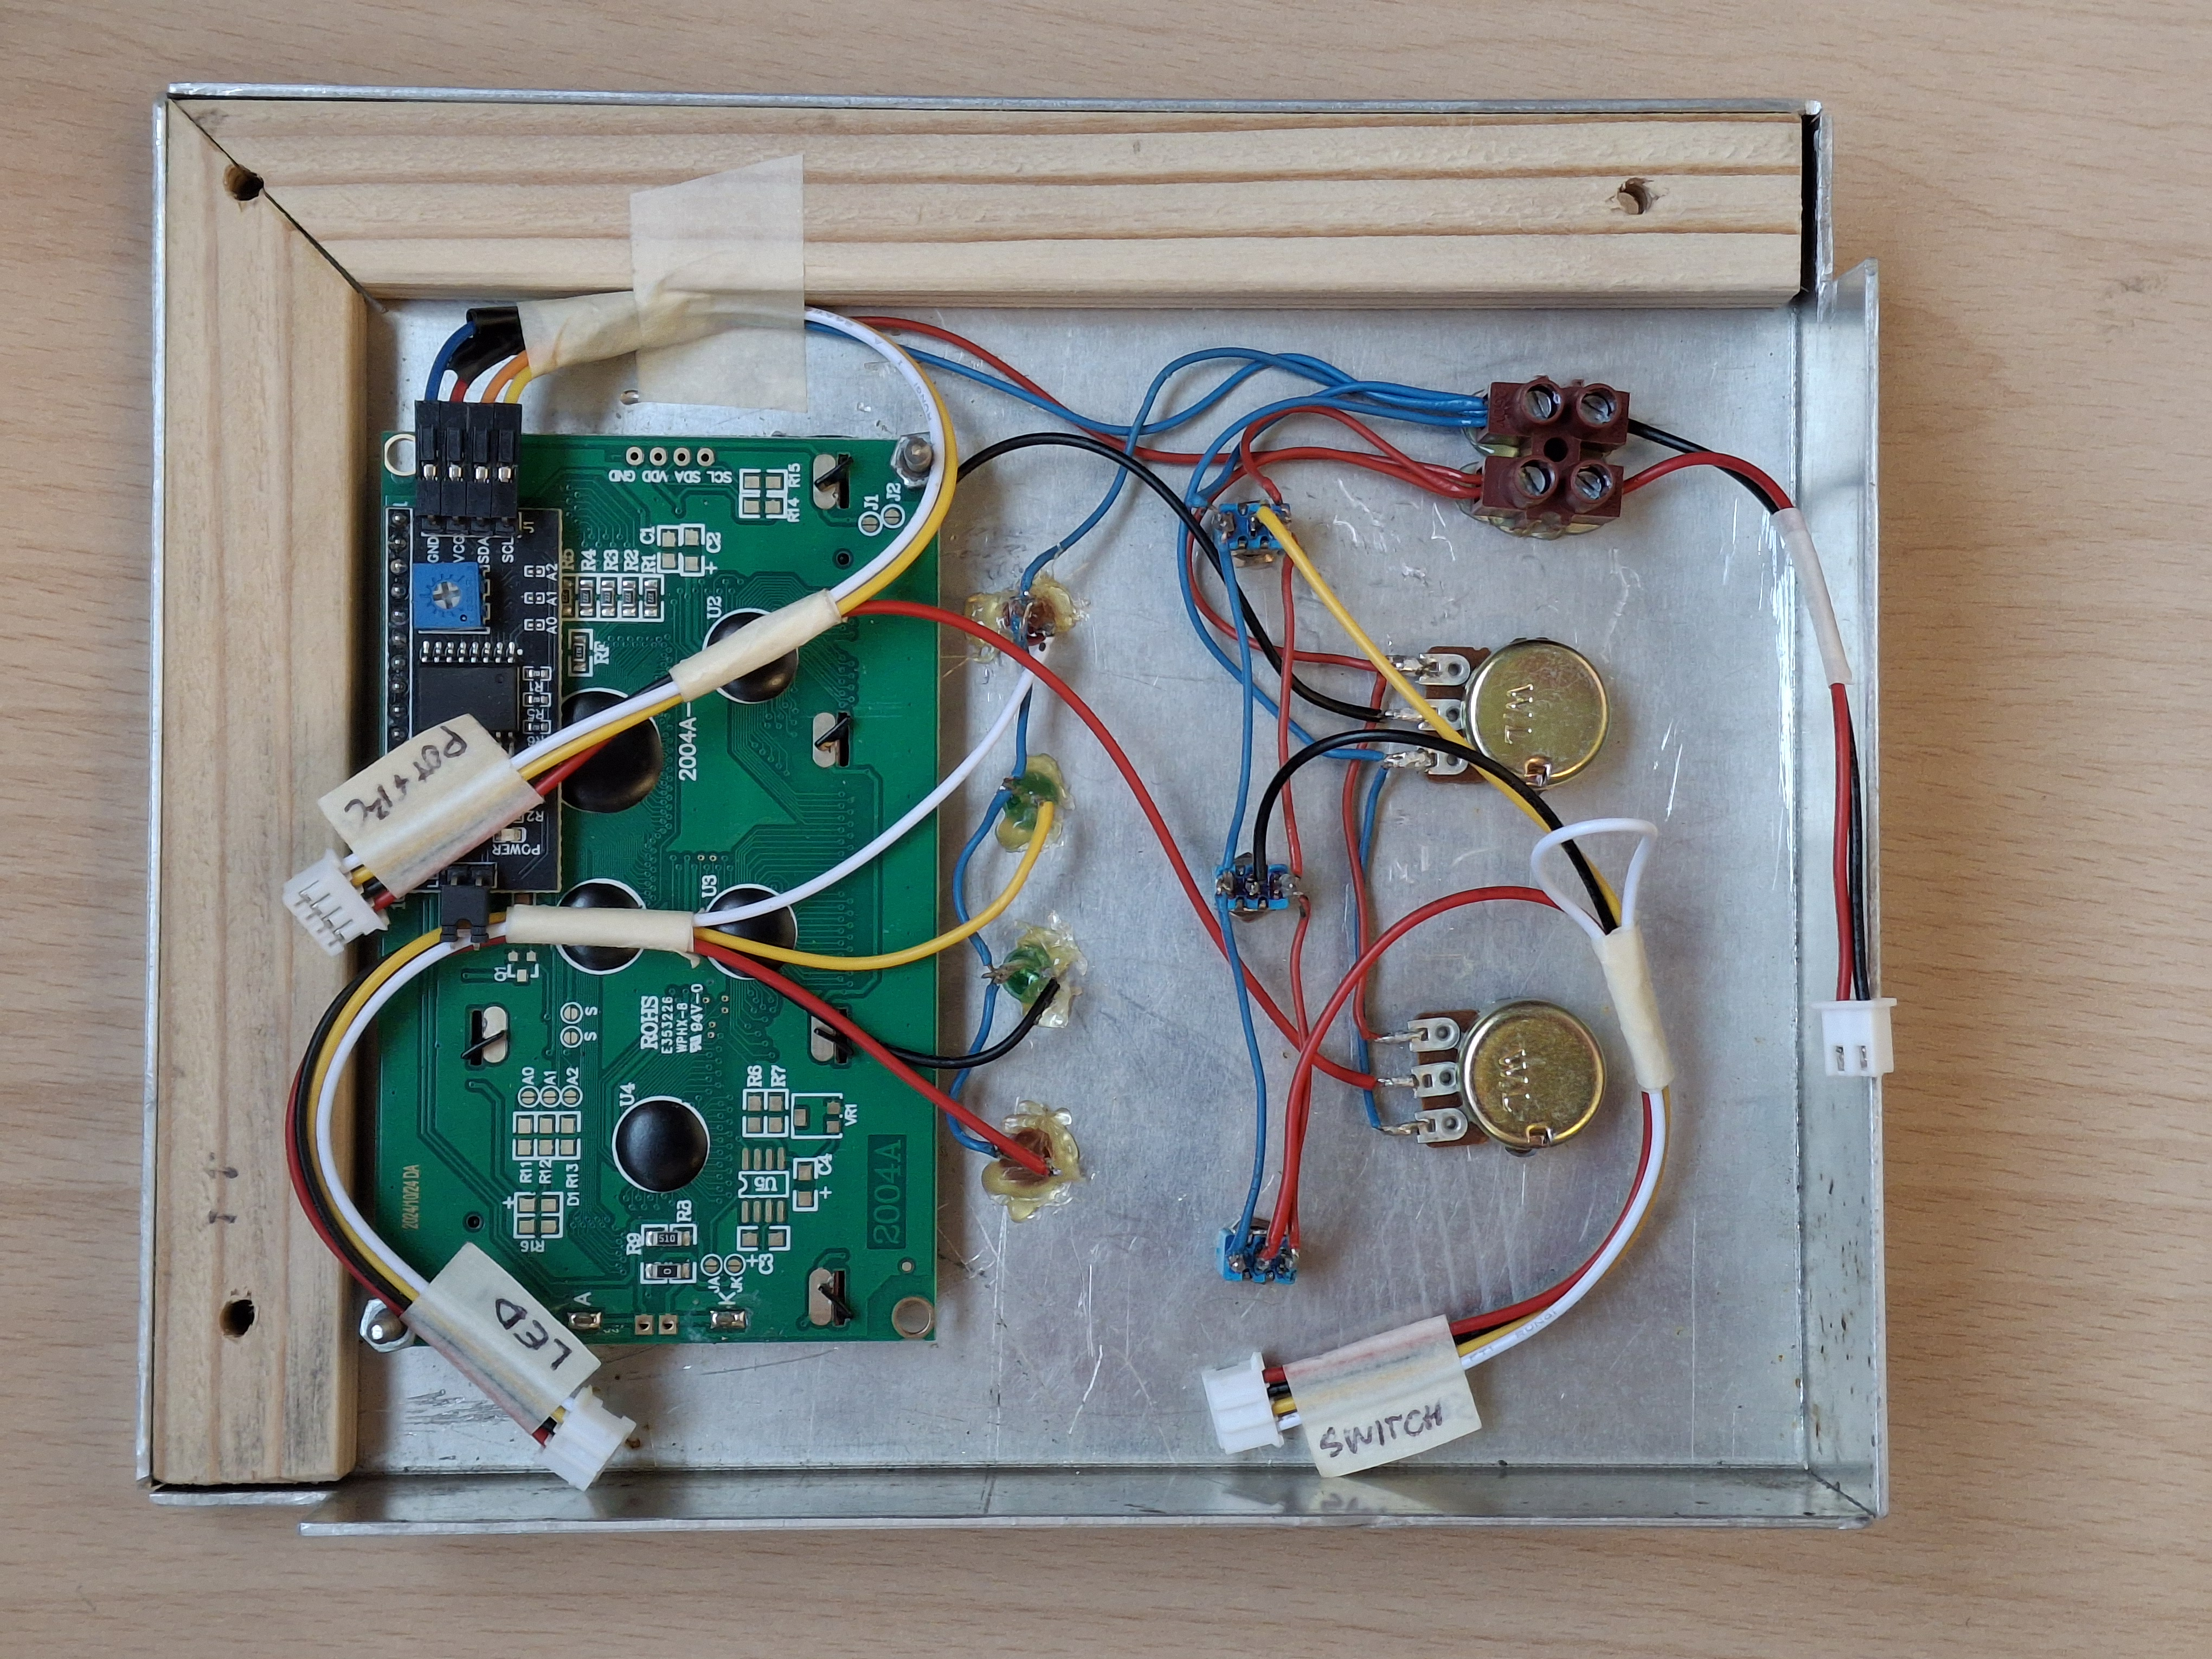
\includegraphics[width=0.9\textwidth]{immagini/1_pannello_frontale_2.png}
    \caption[Foto delle connessioni nel pannello frontale]{Foto delle connessioni tra i vari componenti presenti nel pannello
	frontale del prototipo di incubatrice neonatale.}
    \label{fig:foto_circuito_2}
\end{figure}

\begin{figure}[htbp]
    \centering
    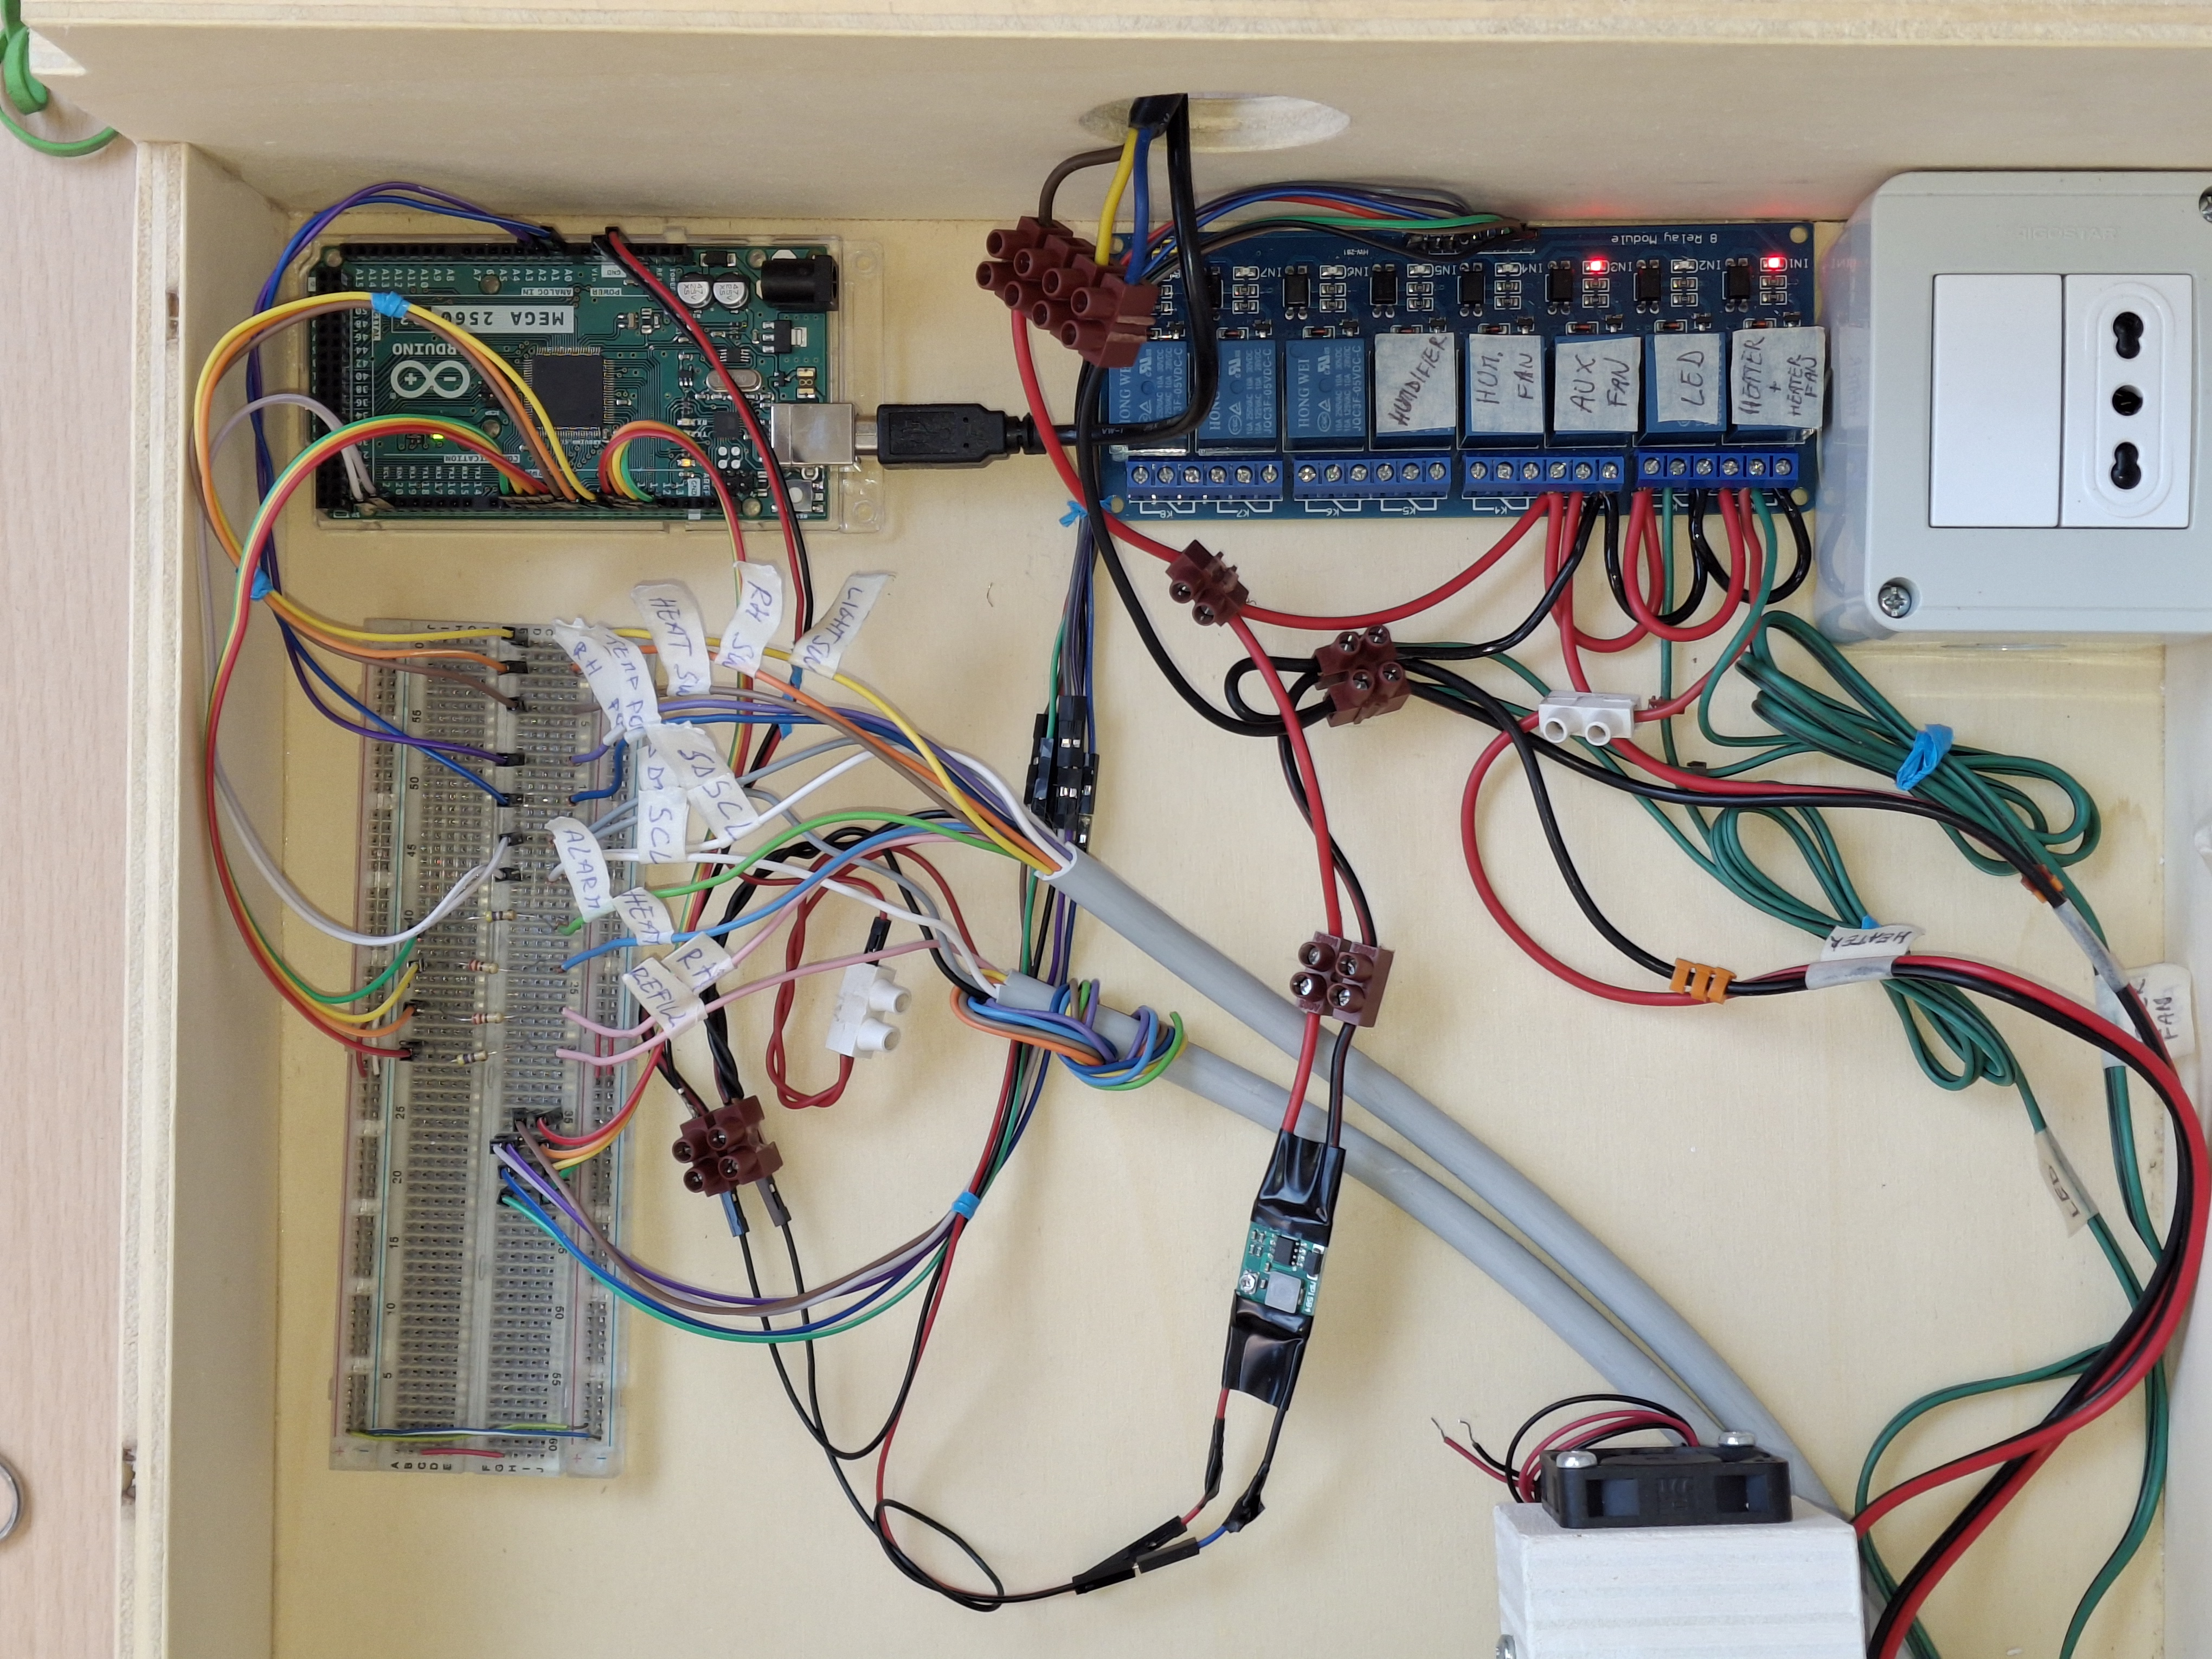
\includegraphics[width=0.9\textwidth]{immagini/1_cassetto.jpg}
    \caption[Foto delle connessioni del cassetto]{Foto delle connessioni presenti nel cassetto inferiore del prototipo di
	incubatrice neonatale in cui si possono notare la scheda Arduino Mega 2560, il modulo relè, lo step down, i cavi provenienti
	dal pannello frontale e dal sensore, la breadboard dove convergono tutti i cavi e il morsetto marrone per la distribuzione
	della massa.}
    \label{fig:foto_circuito_3}
\end{figure}

	\cleardoublepage

	\chapter{Sviluppo del firmware per la gestione dell'incubatrice neonatale}
\section{Requisiti del firmware}
Il firmware per il microcontrollore deve essere in grado di gestire in tempo reale ed in maniera concorrente tutti i
componenti del prototipo di incubatrice neonatale, come il pannello informativo frontale, la gestione degli attuatori,
il sensore di temperatura e umidità, la comunicazione seriale con il PC e i controllori per la gestione della temperatura.

Per garantire la corretta sincronizzazione tra i vari processi, non è possibile impiegare codice bloccante come loop
in attesa di soddisfare una certa condizione o l'utilizzo dela funzione \verb|delay()|. Serve usare un approccio basato
su macchine a stati e condizioni che sfruttano la funzione \verb|millis()|. In questo modo, il microcontrollore può
portare avanti più processi in parallelo senza rimanere occupato a concludere un determinato compito e trascurare gli altri.

Siccome il firmware deve operare su un microcontrollore con risorse limitate, l'implementazione deve essere efficiente
sia in termini di complessità computazionale che di memoria. Per questo motivo, si cerca di limitare il più possibile
l'uso di variabili locali e di allocazioni dinamiche nello stack/heap, preferendo l'uso di variabili globali. In questo
modo la memoria RAM utilizzata per le variabili è già conosciuta a tempo di compilazione e risulta facile accorgersi di
possibili problemi di overflow della memoria. Inoltre, l'uso di variabili globali permette di condividere facilmente
lo stato del sistema tra i vari moduli del firmware, senza dover ricorrere continuamente a passaggi di parametri tra
le funzioni.

Infine è richiesto che il codice sia modulare, leggibile, documentato e facilmente modificabile. Nello sviluppo di un
prototipo orientato alla ricerca, infatti, capiterà sicuramente e molto spesso la necessità di modificare il codice
per aggiungere nuove funzionalità, correggere scelte che si rivelano non ottimali o per adattarlo a nuove esigenze.

\section{Configurazione generale}
\begin{itemize}
	\item variabili globali di stato
	\item files e moduli del firmware
	\item istruzioni di compilazione da arduino ide e platform.io
\end{itemize}

\section{Gestione degli attuatori}
\begin{itemize}
	\item controllo manuale o automatico degli attuatori
	\item gestione centralizzata degli attuatori per aggiornare le variabili di stato
	\item gestione della ventola di omogeneizzazione della temperatura
	\item gestione del refill dell'acqua per il sistema di umidificazione
\end{itemize}

\section{Gestione del pannello frontale}
\begin{itemize}
	\item lettura degli switch, con impostazione controllo manuale
	\item lettura dei potenziometri, con filtri per ridurre il rumore
	\item gestione del display lcd con temporizzazioni
	\item gestione degli errori e gestione del led di allarme
\end{itemize}

\section{Gestione della comunicazione seriale al PC}
\begin{itemize}
	\item comunicazioni seriali
	\item codice matlab
\end{itemize}

\section{Gestione del sensore di temperatura e umidità}
\begin{itemize}
	\item gestione non bloccante
	\item utilizzo di una macchina a stati
\end{itemize}

	\cleardoublepage

	\chapter{Sviluppo del controllore di temperatura per l'incubatrice neonatale}
\section{Requisiti del controllore di temperatura}
Per poter essere immessa sul mercato, un’incubatrice neonatale deve soddisfare i requisiti previsti da diverse normative
tecniche, tra cui la norma ``IEC 60601-2-19'' \cite{iec_60601_2_19}, sviluppata dalla IEC (International Electrotechnical
Commission), che costituisce il principale riferimento internazionale per questa tipologia di dispositivi. La norma è stata
successivamente recepita in ambito europeo dal CEN (Comitato europeo di normazione) e dal CENELEC (Comitato europeo di
normazione elettrotecnica), dando origine alla norma ``EN IEC 60601-2-19''.

Per la progettazione del controllore è stata assunta come riferimento la versione britannica della norma,
``BS EN IEC 60601-2-19:2021+A1:2023'' \cite{bs_60601_2_19}. Tale documento è tecnicamente identico alla norma
``IEC 60601-2-19:2020'' con l'integrazione dell'emendamento A1:2023.

Analizzando le parti relative al controllo della temperatura delle incubatrici neonatali, si possono individuare i seguenti
requisiti principali:

\begin{itemize}
	\item sensore posizionato al centro della culla, a 10 cm dalla base del materasso
	\item funzionalità del controllore con temperature esterne comprese tra i 20°C e i 30°C
	\item setpoint compreso tra 35 e 37°C, almeno 3°C sopra la temperatura ambiente
	\item il setpoint impostabile dall'operatore non deve superare i 37°C, è permesso impostare una temperatura fino
	a 39°C, ma la norma impone che questo avvenga esclusivamente tramite un'azione intenzionale e separata da parte
	dell'operatore
	\item warm-up time: tempo impiegato per arrivare a +11°C dalla temperatura ambiente, ad esempio 25°C -> 36°C, deve
	rientrare entro il 20\% del valore dichiarato nelle istruzioni
	\item una volta raggiunta la temperatura target (Steady Temperature Condition - STC), questa non deve variare per
	più di 1°C nell'arco di un'ora, micro fluttuazioni di 0.5°C sono ammesse
	\item overshoot transitorio non deve superare i 2°C
	\item riacquisizione della condizione di regime (steady state) entro 15 minuti da un eventuale disturbo
\end{itemize}

\section{Controllore ad isteresi}
\subsection{Principio di funzionamento di un controllore ad isteresi}
\subsection{Implementazione del controllore ad isteresi nel firmware}
\subsection{Test di funzionamento con grafico e prestazioni}

\begin{figure}[htbp]
	\centering
	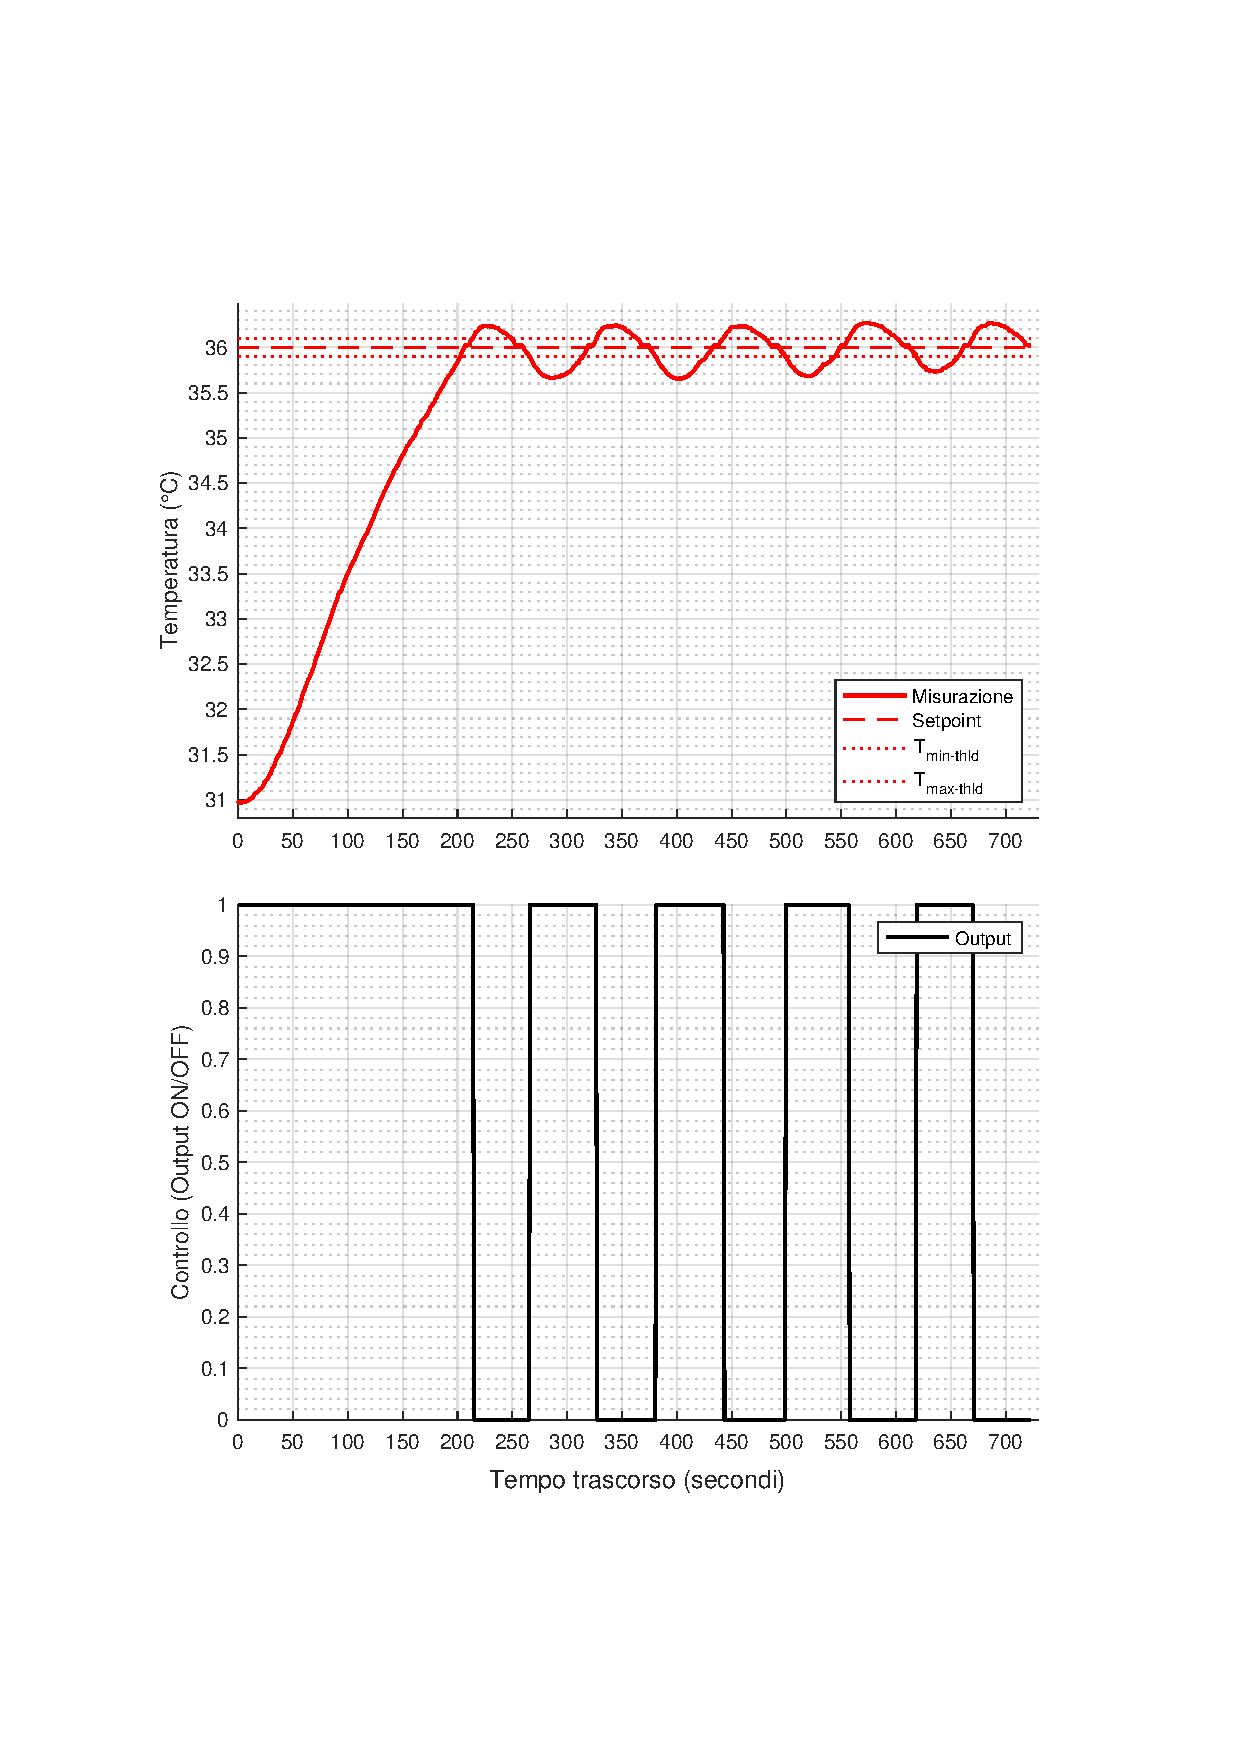
\includegraphics[width=0.9\textwidth, trim={2.5cm 4cm 2.5cm 4cm}, clip]{immagini/3_isteresi.pdf}
	\caption[Grafico del setpoint del controllore ad isteresi]{Grafico del raggiungimento e mantenimento del setpoint
	di temperatura ottenuto con il controllore ad isteresi.}
	\label{fig:isteresi}
\end{figure}

\newpage

\section{Controllore PID}
\subsection{Principio di funzionamento di un controllore PID}
\subsection{Implementazione del controllore PID nel firmware}
\subsubsection{Salvataggio degli errori e delle misurazioni nel buffer}
\subsubsection{Aggiornamento dello stato}
\subsubsection{Gestione del ciclo pwm}
\subsubsection{Sistema di anti-windup}
\subsubsection{Derivative on measurement}
\subsection{Test di funzionamento con grafico e prestazioni}


parametri ottimali individuati:
\begin{itemize}
	\item kp = 55, ki = 0.40, kd = 1000
	\item kp = 55, ki = 0.35, kd = 1200
	\item kp = 60, ki = 0.4, kd = 1500
\end{itemize}

prestazioni richieste:
\begin{itemize}
	\item rise time
	\item settling time
	\item overshoot
\end{itemize}

\begin{figure}[htbp]
	\centering
	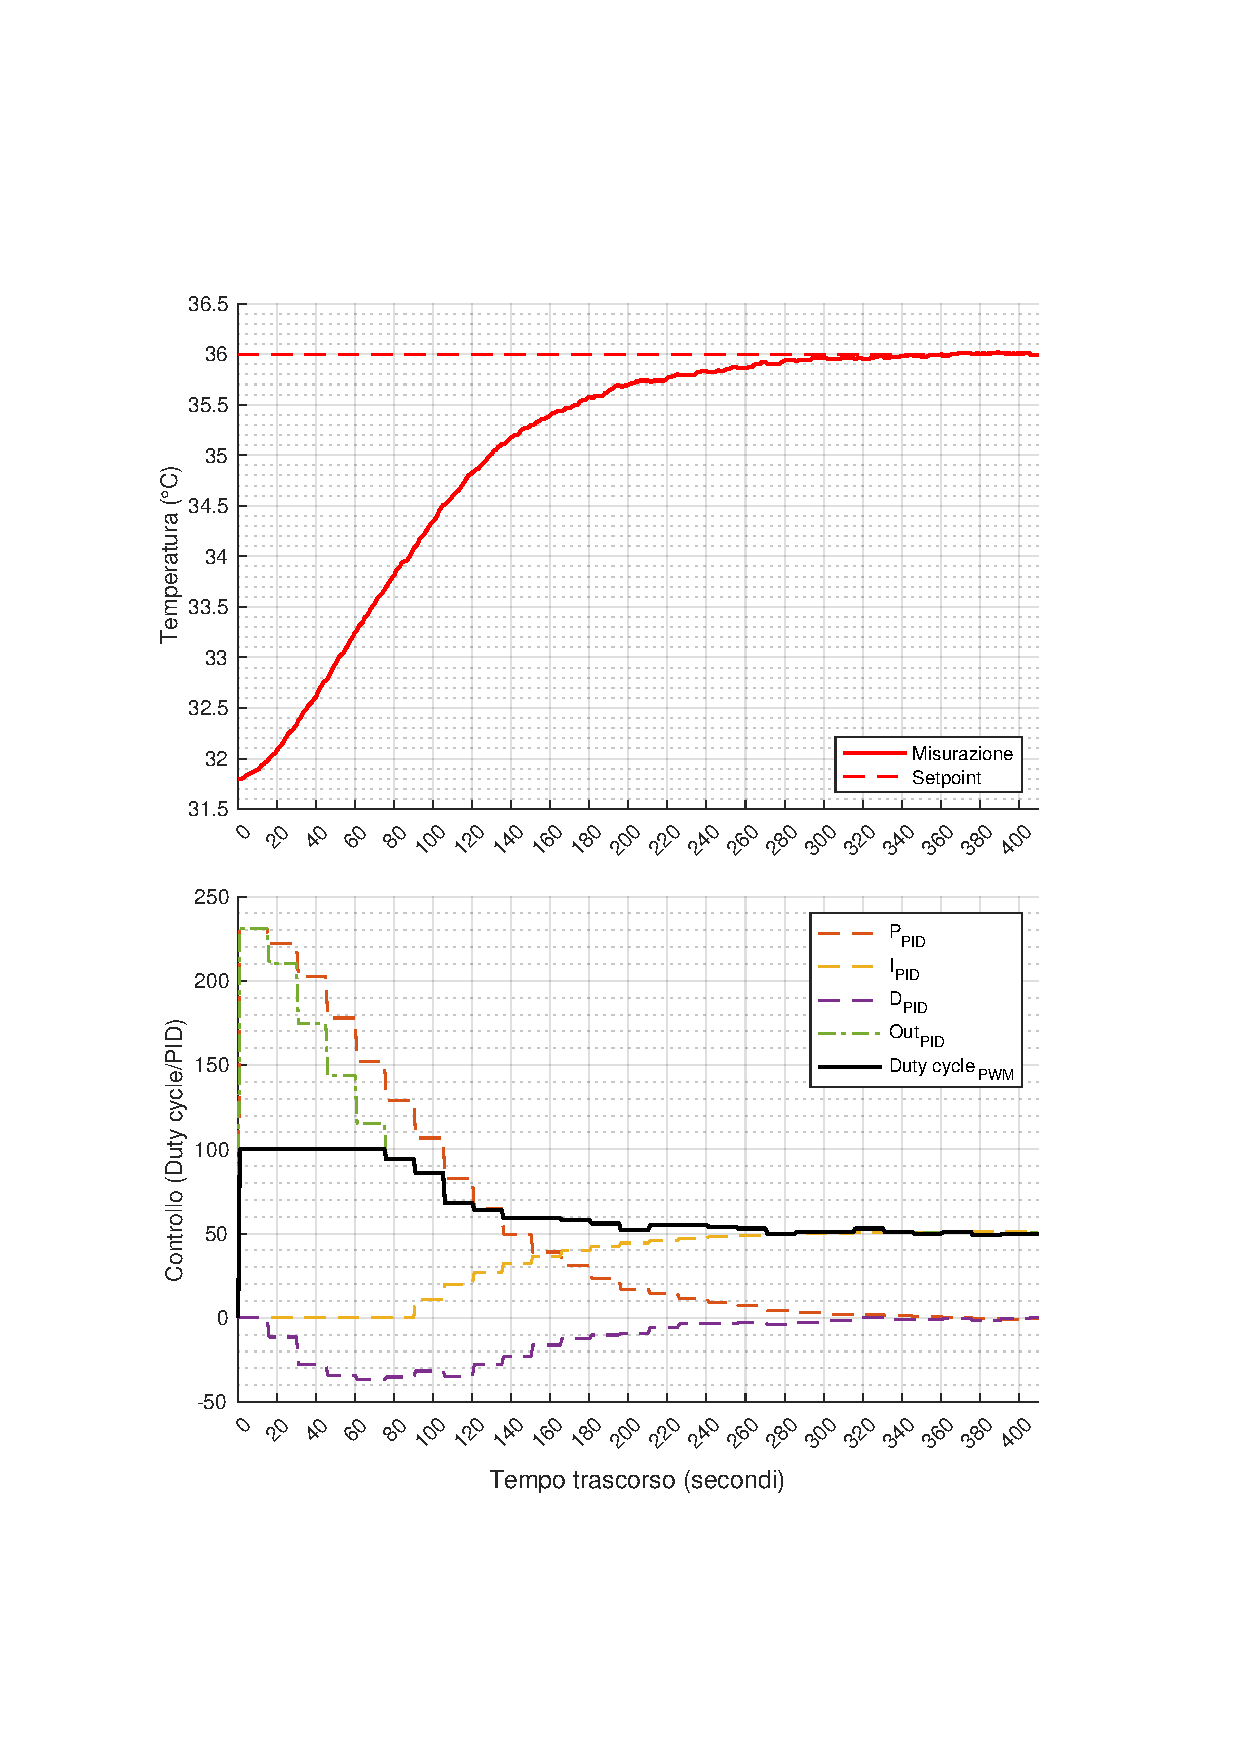
\includegraphics[width=0.9\textwidth, trim={2.5cm 4cm 2.5cm 4cm}, clip]{immagini/3_pid_1_1.pdf}
	\caption[Grafico del setpoint del controllore PID]{Grafico del raggiungimento e mantenimento del setpoint di temperatura
	ottenuto con il controllore PID con parametri Kp=55, Ki=0.35, Kd=1200.}
	\label{fig:pid_gradino}
\end{figure}

\begin{figure}[htbp]
	\centering
	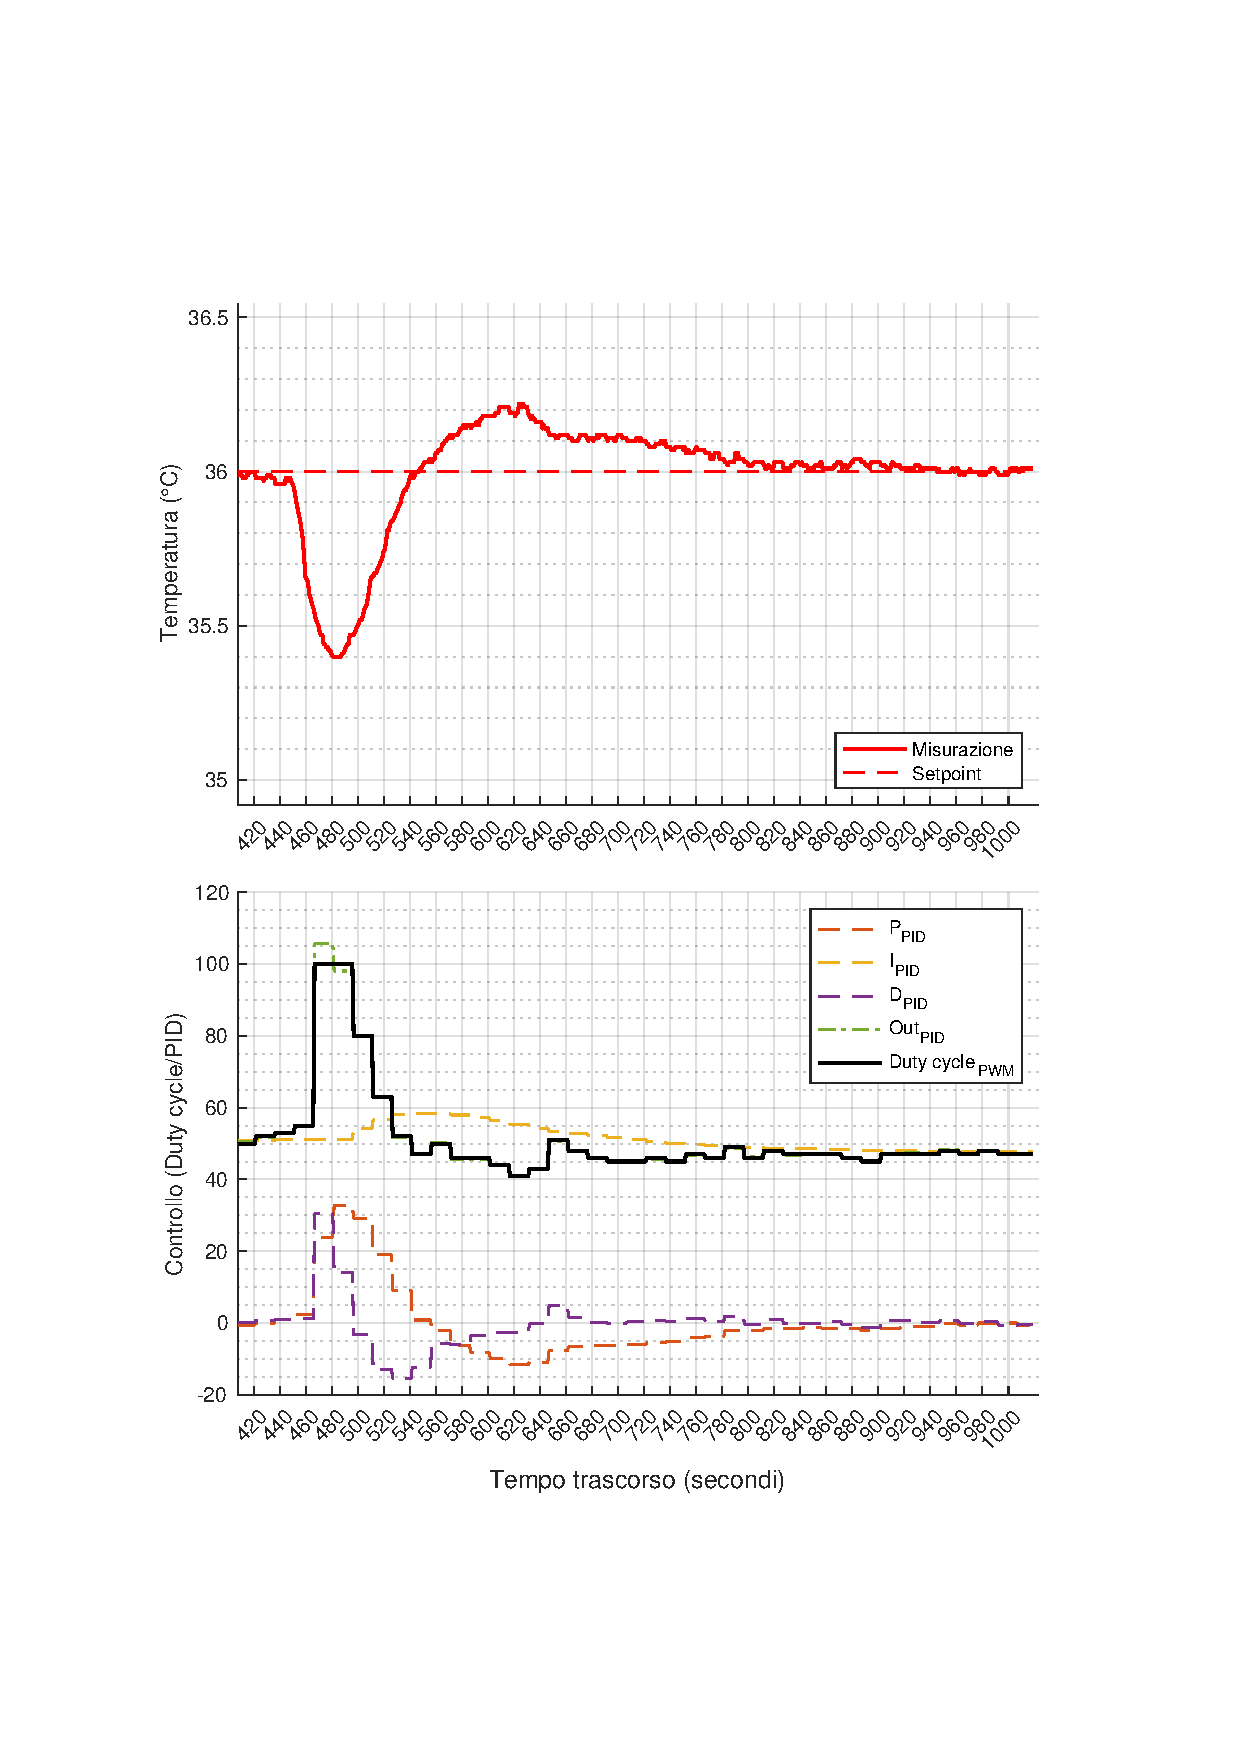
\includegraphics[width=0.9\textwidth, trim={2.5cm 4cm 2.5cm 4cm}, clip]{immagini/3_pid_1_2.pdf}
	\caption[Grafico della perturbazione del controllore PID]{Grafico del ripristino del setpoint di temperatura dopo un
	disturbo esterno, ottenuto con il controllore PID con parametri Kp=55, Ki=0.35, Kd=1200.}
	\label{fig:pid_perturbazione}
\end{figure}

\section{Confronto tra controllore ad isteresi e PID}

	\cleardoublepage

	\chapter{Conclusioni}
\section{Discussione critica dei risultati ottenuti}
\begin{itemize}
	\item sviluppo del codice firmware, durata media e massima di un loop
	\item taratura dei parametri e conoscenza dei limiti del controllore PID
	\item miglioramenti del pid rispetto al controllore ad isteresi
\end{itemize}

\section{Possibili sviluppi futuri}
\begin{itemize}
	\item implementazione di un sistema di controllo dell'umidità (o controllo multivariabile)
	\item valutare se implementare il pid per farlo lavorare su interi e non float, stando attenti agli overflow
	\item utilizzare mosfet al posto dei relè e aggiungere un sistema di smorzamento dell'output alla riattivazione
	del pid
	\item modellare il sistema per implementare un controllore dal punto di vista teorico con simulazioni e poi
	testare i parametri ottimali sul prototipo reale
	\item integrare un'azione di feedforward (considerando l'inerzia termica) e attivare il pid solo a regime
	\item campo di prova per implementare e testare altri tipi di controllore (ad esempio fuzzy, predittivo, ecc.)
\end{itemize}

	\cleardoublepage

	\appendix
\chapter{Metodo dei minimi quadrati per il calcolo stabile della derivata}
\label{chap:derivata_regressione_lineare}
Di seguito viene illustrato il procedimento matematico effettuato per ottenere la formula utilizzata nel controllore PID per
il calcolo del contributo derivativo attraverso una regressione lineare sui dati contenuti nel buffer.

Il calcolo della derivata di una grandezza fisica misurata da un sensore risulta particolarmente delicato in quanto è fortemente
soggetto al rumore delle misurazioni. Il semplice calcolo del rapporto incrementale tra due campioni consecutivi può portare
a rapide variazioni della derivata che potrebbero indurre problemi di stabilità del controllore. Per mitigare le fluttuazioni
istantanee si è scelto di utilizzare il metodo dei minimi quadrati ed effettuare una regressione lineare su un set più ampio
di dati in modo da compensare le fluttuazioni istantanee e ottenere una stima più stabile della derivata.

\subsection*{Notazioni e convenzioni utilizzate}
Nei calcoli successivi si adottano le seguenti notazioni:
\begin{itemize}
	\item \(y_i\) : misurazione del sensore all'istante di tempo \(x_i\)
	\item \(a_0 + a_1 \, x_i\) : retta di regressione lineare, dove \(a_0\) è intercetta e \(a_1\) è il coefficiente angolare
	della retta di regressione lineare, che rappresenta la derivata da calcolare
\end{itemize}

Per calcolare la derivata ad un certo istante di tempo \(x_i\), si considerano solo gli ultimi \(N\) campioni misurati dal
sensore. Scelto \(x_k\) l'istante di tempo associato all'ultima misurazione \(y_j\), l'indice \(i\) dei campioni considerati
varia in \([j \!-\! (N \!-\! 1), \, j]\) con \(j \in \mathbb{N}\). Siccome gli indici delle sommatorie sono variabili mute,
nei successivi passaggi si considera senza perdita di generalità \(j = N \!-\! 1\) in modo che \(i\) varia da \(0\) a \(N-1\).

\subsection*{Procedimento matematico}
L'errore \(e_i\) tra la misurazione \(y_i\) e la retta di regressione lineare \(a_0 + a_1 \, x_i\) viene definito come:
\begin{equation}
	e_i = y_i - (a_0 + a_1 \, x_i)
\end{equation}

Si definisce quindi l'errore quadratico totale \(S(a_0, a_1)\) come segue:
\begin{equation}
	S(a_0, a_1) \; = \; \sum_{i = 0}^{N-1} e_i^2 \; = \; \sum_{i = 0}^{N-1} (y_i - (a_0 + a_1 \, x_i))^2
\end{equation}

I parametri \(a_0\) e \(a_1\) della retta di regressione lineare che minimizzano l'errore quadratico totale \(S(a_0, a_1)\)
si ottengono ponendo a zero le derivate parziali di \(S(a_0, a_1)\) rispetto a \(a_0\) e \(a_1\) e risolvendo il sistema
lineare di due equazioni a due incognite \(a_0\) e \(a_1\) così ottenuto.
\begin{align}
	\frac{\partial S(a_0, a_1)}{\partial a_0} &= -2 \sum_{i = 0}^{N-1} (y_i - (a_0 + a_1 \, x_i)) = \\
	&= -2 \left( \sum_{i = 0}^{N-1} y_i - \sum_{i=0}^{N-1} a_0 - \sum_{i=0}^{N-1} a_1 \, x_i \right) = \\
	&= -2 \left( \sum_{i = 0}^{N-1} y_i - a_0 \sum_{i=0}^{N-1} 1 - a_1 \sum_{i=0}^{N-1} x_i \right) = \\
	&= -2 \left( N \bar{y} - a_0 N - a_1 N \bar{x} \right) = \\
	&= -2 N \left( \bar{y} - a_0 - a_1 \bar{x} \right)
\end{align}
\begin{align}
	\frac{\partial S(a_0, a_1)}{\partial a_1} &= -2 \sum_{i = 0}^{N-1} x_i (y_i - (a_0 + a_1 \, x_i)) = \\
	&= -2 \left( \sum_{i = 0}^{N-1} x_i y_i - \sum_{i=0}^{N-1} a_0 x_i - \sum_{i=0}^{N-1} a_1 {x_i}^2 \right) = \\
	&= -2 \left( \sum_{i = 0}^{N-1} x_i y_i - a_0 \sum_{i=0}^{N-1} x_i - a_1 \sum_{i=0}^{N-1} {x_i}^2 \right) = \\
	&= -2 \left( \sum_{i = 0}^{N-1} x_i y_i - a_0 N \bar{x} - a_1 \sum_{i=0}^{N-1} {x_i}^2 \right)
\end{align}

\newpage

Si procede quindi a risolvere il sistema di equazioni lineari così ottenuto per sostituzione:
\begin{equation}
	\begin{cases}
		\frac{\partial S(a_0, a_1)}{\partial a_0} = 0 \\
		\frac{\partial S(a_0, a_1)}{\partial a_1} = 0
	\end{cases}
	\quad \Rightarrow \quad
	\begin{cases}
		2 N \left( \bar{y} - a_0 - a_1 \bar{x} \right) = 0 \\
		-2 \left( \sum_{i = 0}^{N-1} x_i y_i - a_0 N \bar{x} - a_1 \sum_{i=0}^{N-1} {x_i}^2 \right) = 0
	\end{cases}
\end{equation}

\begin{equation}
	-2 N \left( \bar{y} - a_0 - a_1 \bar{x} \right) = 0 \quad \Rightarrow \quad a_0 = \bar{y} - a_1 \bar{x}
\end{equation}
\begin{align}
	-2 \left( \sum_{i = 0}^{N-1} x_i y_i - a_0 N \bar{x} - a_1 \sum_{i=0}^{N-1} {x_i}^2 \right) = 0 \\
	\sum_{i = 0}^{N-1} x_i y_i - (\bar{y} - a_1 \bar{x}) N \bar{x} - a_1 \sum_{i=0}^{N-1} {x_i}^2 = 0 \\
	\sum_{i = 0}^{N-1} x_i y_i - N \bar{y} \bar{x} + a_1 N {\bar{x}}^2 - a_1 \sum_{i=0}^{N-1} {x_i}^2 = 0 \\
	\sum_{i = 0}^{N-1} x_i y_i - N \bar{y} \bar{x} - a_1 \left( \sum_{i=0}^{N-1} {x_i}^2 - N {\bar{x}}^2 \right) = 0 \\
\end{align}
\begin{equation}
	a_1 = \frac{\displaystyle \;\; \sum_{i=0}^{N-1} x_i y_i - N \bar{y} \bar{x} \;\;}{\displaystyle \;\; \sum_{i=0}^{N-1} {x_i}^2 - N {\bar{x}}^2 \;\;} \label{eq:7_a1_base}
\end{equation}

Si assume che gli istanti di tempo \(x_i\) sono tutti equidistanti, ovvero che formano una sequenza continua dei multipli del
tempo di campionamento \(T_s\) a partire dall'istante iniziale \(k \, T_s\) dove \(k = j - (N - 1)\). I campioni \(x_i\) possono
essere quindi espressi in funzione dei due indici \(i\) e \(k\):
\begin{equation}
	x_i = (j - (N-1)) \, T_s + i \, T_s = (k + i) \, T_s \qquad \text{con} \; \bar{x} = \frac{1}{N} \sum_{i=0}^{N-1} x_i = \frac{T_s}{N} \sum_{i=0}^{N-1} (k + i)\label{eq:7_sub}
\end{equation}

È possibile quindi riscrivere la formula \eqref{eq:7_a1_base} con la sostituzione \eqref{eq:7_sub} individuata sopra:
\begin{equation}
	a_1 = \frac{\displaystyle \;\; T_s \sum_{i=0}^{N-1} (k + i) \, y_i - N \bar{y} \left(\frac{T_s}{N} \, \sum_{i=0}^{N-1} (k + i)\right) \;\;}{\displaystyle \;\; {T_s}^2 \sum_{i=0}^{N-1} (k + i)^2 - N \left(\frac{T_s}{N} \,\sum_{i=0}^{N-1} (k + i)\right)^2 \;\;}
\end{equation}

\newpage

Analizzando separatamente il numeratore e il denominatore della formula \eqref{eq:7_a1_base} si ottengono le seguenti
semplificazioni fino ad ottenere la formula finale utilizzata nell'implementazione del controllore PID:
\begin{align}
	\textit{Num.} &= T_s \sum_{i=0}^{N-1} (k + i) \, y_i - N \bar{y} \left(\frac{T_s}{N} \, \sum_{i=0}^{N-1} (k + i)\right) = \\
	&= T_s \left(k \sum_{i=0}^{N-1} y_i + \sum_{i=0}^{N-1} i \cdot y_i\right) - N \bar{y} \cdot \frac{T_s}{N} \cdot \left( \sum_{i=0}^{N-1} i + \sum_{i=0}^{N-1} k \right) = \\
	&= T_s \left( k N \bar{y} + \sum_{i=0}^{N-1} i \cdot y_i - \bar{y} \left(\frac{N(N-1)}{2} + kN\right) \right) = \\
	&= T_s \left( k N \bar{y} + \sum_{i=0}^{N-1} i \cdot y_i - \frac{N(N-1)}{2} \cdot \bar{y} - k N \bar{y} \right) = \\
	&= T_s \left( \sum_{i=0}^{N-1} i \cdot y_i - \frac{N(N-1)}{2} \cdot \bar{y} \right) = \\
	&= T_s \left( \sum_{i=0}^{N-1} i \cdot y_i - \frac{N-1}{2} \cdot \sum_{i=0}^{N-1} y_i \right) \label{eq:7_num}
\end{align}
\begin{align}
	\textit{Den.} &= {T_s}^2 \sum_{i=0}^{N-1} (k + i)^2 - N \left(\frac{T_s}{N} \,\sum_{i=0}^{N-1} (k + i)\right)^2 = \\
	&= {T_s}^2 \left( \sum_{i=0}^{N-1} (k^2 + 2ik + i^2) - \frac{1}{N} \left( \sum_{i=0}^{N-1} (k + i) \right)^2 \right) = \\
	&= {T_s}^2 \left( k^2 N + 2k \sum_{i=0}^{N-1} i + \sum_{i=0}^{N-1} i^2 - \frac{1}{N} \left( k N + \sum_{i=0}^{N-1} i \right)^2 \right) = \\
	&= {T_s}^2 \left( k^2 N \!+\! 2k \frac{N(N\!\!-\!\!1)}{2} \!+\! \frac{N(N\!\!-\!\!1)(2N\!\!-\!\!1)}{6} - \frac{1}{N} \left( k N \!+\! \frac{N(N\!\!-\!\!1)}{2} \right)^2 \right) = \\
	\begin{split}
		&= {T_s}^2 \bigg( k^2 N + k N^2 - kN + \frac{2N^3 - 3 N^2 + N}{6} + \\[-5pt]
		&\qquad\qquad\qquad\qquad -\frac{1}{N} \cdot \bigg( k^2 N^2 + kN^3 - kN^2 + \frac{N^4 - 2N^3 + N^2}{4} \bigg) \bigg) = \\
	\end{split} \\
	\begin{split}
		&= \frac{{T_s}^2}{12} \cdot \big( 12k^2 N + 12k N^2 - 12kN + 4N^3 - 6N^2 + 2N + \\
		&\qquad\qquad\qquad\qquad + 12k^2 N - 12k N^2 + 12kN - 3N^3 + 6N^2 - 3N \big) =
	\end{split} \\
	&= \frac{{T_s}^2}{12} \left( N^3 - N \right) = \frac{{T_s}^2}{12} \cdot N (N-1)(N+1) \label{eq:7_den}
\end{align}


Unendo i due termini \eqref{eq:7_num} e \eqref{eq:7_den} così ottenuti, si arriva alla formula finale utilizzata
nell'implementazione del controllore PID.
\begin{align}
	a_1 &= \frac{\displaystyle \;\; T_s \sum_{i=0}^{N-1} (k + i) \, y_i - N \bar{y} \left(\frac{T_s}{N} \, \sum_{i=0}^{N-1} (k + i)\right) \;\;}{\displaystyle \;\; {T_s}^2 \sum_{i=0}^{N-1} (k + i)^2 - N \left(\frac{T_s}{N} \,\sum_{i=0}^{N-1} (k + i)\right)^2 \;\;} = \\[5pt]
	&= \frac{\displaystyle \;\; T_s \left( \sum_{i=0}^{N-1} i \cdot y_i - \frac{N-1}{2} \cdot \sum_{i=0}^{N-1} y_i \right) \;\;}{\displaystyle \;\; \frac{{T_s}^2}{12} \cdot N (N-1)(N+1) \;\;} = \\[5pt]
	&= \frac{12}{T_s \cdot N(N-1)(N+1)} \cdot \left( \sum_{i=0}^{N-1} i \cdot y_i - \frac{N-1}{2} \cdot \sum_{i=0}^{N-1} y_i \right) = \\
	&= \frac{12}{T_s \cdot N(N^2-1)} \cdot \sum_{i=0}^{N-1} i \cdot y_i - \frac{6}{T_s \cdot N(N+1)} \cdot \sum_{i=0}^{N-1} y_i
\end{align}


% -------------------------------------------------------------------------------------------------
% ------------- codice con verbatim se è richiesto il formato PDF/A-1a (accessibile) --------------
% -------------------------------------------------------------------------------------------------
%
% Per utilizzare correttamente il sistema di tagging dei listing richiesto dallo standard
% PDF/A-1a (accessibile) non è possibile utilizzare il comando \captionof{}{} al di fuori
% di ambienti flottanti. Per questo motivo, si riporta di seguito il procedimento da seguire
% in 5 fasi principali:
%
%  1. incremento del contatore dei listing
%     \noindent\refstepcounter{lstlisting}
%
%  2. creazione della reference per il listing
%	  \label{lst:label_del_listing}
%
%  3. stampa della didascalia del listing
%     \noindent\text{Codice \thelstlisting: Didascalia del listing}
%
%  4. aggiunta del listing all'indice dei listing
%     \addcontentsline{lol}{lstlisting}{\protect\numberline{\thelstlisting}Didascalia del listing}
%
%  5. importazione del file di codice con verbatim aggiungendo le linee orizzontali sopra e sotto il codice
%     per una migliore leggibilità e con dimensione del font ridotta
%     \noindent\rule{\textwidth}{0.4pt}
%     {\scriptsize \verbatiminput{percorso_del_file}}
%     \noindent\rule{\textwidth}{0.4pt}
%

%\chapter{Codice del firmware}
%\section{File di configurazione per PlatformIO in VSCode}
%
%% etichetta file di configurazione dell'ambiente PlatformIO in VSCode
%\noindent\refstepcounter{lstlisting}
%\label{lst:platformio_ini}
%\noindent\text{Codice \thelstlisting: File di configurazione dell'ambiente PlatformIO in VSCode}
%\addcontentsline{lol}{lstlisting}{\protect\numberline{\thelstlisting}File di configurazione dell'ambiente PlatformIO in VSCode}
%
%% codice del file di configurazione dell'ambiente PlatformIO in VSCode
%\noindent\rule{\textwidth}{0.4pt}
%{\tiny \verbatiminput{../programmi/firmware/platformio.ini}}
%\noindent\rule{\textwidth}{0.4pt}
%
%\section{File di configurazione del firmware}
%
%% etichetta file header con i parametri di configurazione
%\noindent\refstepcounter{lstlisting}
%\label{lst:config_h}
%\noindent\text{Codice \thelstlisting: File header con i parametri di configurazione}
%\addcontentsline{lol}{lstlisting}{\protect\numberline{\thelstlisting}File header con i parametri di configurazione}
%
%% codice del file header con i parametri di configurazione
%\noindent\rule{\textwidth}{0.4pt}
%{\tiny \verbatiminput{../programmi/firmware/lib/config/config.h}}
%\noindent\rule{\textwidth}{0.4pt}
%
%% etichetta file sorgente con i parametri di configurazione
%\noindent\refstepcounter{lstlisting}
%\label{lst:config_cpp}
%\noindent\text{Codice \thelstlisting: File sorgente con i parametri di configurazione}
%\addcontentsline{lol}{lstlisting}{\protect\numberline{\thelstlisting}File sorgente con i parametri di configurazione}
%
%% codice del file sorgente con i parametri di configurazione
%\noindent\rule{\textwidth}{0.4pt}
%{\tiny \verbatiminput{../programmi/firmware/lib/config/config.cpp}}
%\noindent\rule{\textwidth}{0.4pt}
%
%\newpage
%
%\section{File del modulo con le funzioni di utilità}
%
%% etichetta file header con le funzioni di utilità
%\noindent\refstepcounter{lstlisting}
%\label{lst:utils_h}
%\noindent\text{Codice \thelstlisting: File header con le funzioni di utilità}
%\addcontentsline{lol}{lstlisting}{\protect\numberline{\thelstlisting}File header con le funzioni di utilità}
%
%% codice del file header con le funzioni di utilità
%\noindent\rule{\textwidth}{0.4pt}
%{\tiny \verbatiminput{../programmi/firmware/lib/utils/utils.h}}
%\noindent\rule{\textwidth}{0.4pt}
%
%% etichetta file sorgente con le funzioni di utilità
%\noindent\refstepcounter{lstlisting}
%\label{lst:utils_cpp}
%\noindent\text{Codice \thelstlisting: File sorgente con le funzioni di utilità}
%\addcontentsline{lol}{lstlisting}{\protect\numberline{\thelstlisting}File sorgente con le funzioni di utilità}
%
%% codice del file sorgente con le funzioni di utilità
%\noindent\rule{\textwidth}{0.4pt}
%{\tiny \verbatiminput{../programmi/firmware/lib/utils/utils.cpp}}
%\noindent\rule{\textwidth}{0.4pt}
%
%\newpage
%
%\section{File del modulo per la gestione degli errori}
%
%% etichetta file header con le funzioni per la gestione degli errori
%\noindent\refstepcounter{lstlisting}
%\label{lst:error_h}
%\noindent\text{Codice \thelstlisting: File header con le funzioni per la gestione degli errori}
%\addcontentsline{lol}{lstlisting}{\protect\numberline{\thelstlisting}File header con le funzioni per la gestione degli errori}
%
%% codice del file header con le funzioni per la gestione degli errori
%\noindent\rule{\textwidth}{0.4pt}
%{\tiny \verbatiminput{../programmi/firmware/lib/error/error.h}}
%\noindent\rule{\textwidth}{0.4pt}
%
%% etichetta file sorgente con le funzioni per la gestione degli errori
%\noindent\refstepcounter{lstlisting}
%\label{lst:error_cpp}
%\noindent\text{Codice \thelstlisting: File sorgente con le funzioni per la gestione degli errori}
%\addcontentsline{lol}{lstlisting}{\protect\numberline{\thelstlisting}File sorgente con le funzioni per la gestione degli errori}
%
%% codice del file sorgente con le funzioni per la gestione degli errori
%\noindent\rule{\textwidth}{0.4pt}
%{\tiny \verbatiminput{../programmi/firmware/lib/error/error.cpp}}
%\noindent\rule{\textwidth}{0.4pt}
%
%\newpage
%
%\section{File del modulo per il controllo attuatori}
%
%% etichetta file header con le funzioni per il controllo degli attuatori
%\noindent\refstepcounter{lstlisting}
%\label{lst:actuators_h}
%\noindent\text{Codice \thelstlisting: File header con le funzioni per il controllo degli attuatori}
%\addcontentsline{lol}{lstlisting}{\protect\numberline{\thelstlisting}File header con le funzioni per il controllo degli attuatori}
%
%% codice del file header con le funzioni per il controllo degli attuatori
%\noindent\rule{\textwidth}{0.4pt}
%{\tiny \verbatiminput{../programmi/firmware/lib/actuators/actuators.h}}
%\noindent\rule{\textwidth}{0.4pt}
%
%% etichetta file sorgente con le funzioni per il controllo degli attuatori
%\noindent\refstepcounter{lstlisting}
%\label{lst:actuators_cpp}
%\noindent\text{Codice \thelstlisting: File sorgente con le funzioni per il controllo degli attuatori}
%\addcontentsline{lol}{lstlisting}{\protect\numberline{\thelstlisting}File sorgente con le funzioni per il controllo degli attuatori}
%
%% codice del file sorgente con le funzioni per il controllo degli attuatori
%\noindent\rule{\textwidth}{0.4pt}
%{\tiny \verbatiminput{../programmi/firmware/lib/actuators/actuators.cpp}}
%\noindent\rule{\textwidth}{0.4pt}
%
%\newpage
%
%\section{File del modulo per la gestione del display lcd}
%
%% etichetta file header con le funzioni per la gestione del display lcd
%\noindent\refstepcounter{lstlisting}
%\label{lst:lcd_h}
%\noindent\text{Codice \thelstlisting: File header con le funzioni per la gestione del display lcd}
%\addcontentsline{lol}{lstlisting}{\protect\numberline{\thelstlisting}File header con le funzioni per la gestione del display lcd}
%
%% codice del file header con le funzioni per la gestione del display lcd
%\noindent\rule{\textwidth}{0.4pt}
%{\tiny \verbatiminput{../programmi/firmware/lib/lcd/lcd.h}}
%\noindent\rule{\textwidth}{0.4pt}
%
%% etichetta file sorgente con le funzioni per la gestione del display lcd
%\noindent\refstepcounter{lstlisting}
%\label{lst:lcd_cpp}
%\noindent\text{Codice \thelstlisting: File sorgente con le funzioni per la gestione del display lcd}
%\addcontentsline{lol}{lstlisting}{\protect\numberline{\thelstlisting}File sorgente con le funzioni per la gestione del display lcd}
%
%% codice del file sorgente con le funzioni per la gestione del display lcd
%\noindent\rule{\textwidth}{0.4pt}
%{\tiny \verbatiminput{../programmi/firmware/lib/lcd/lcd.cpp}}
%\noindent\rule{\textwidth}{0.4pt}
%
%\newpage
%
%\section{File del modulo per la gestione del sensore di temperatura e umidità SHT20}
%
%% etichetta file header con le funzioni per la gestione del sensore SHT20
%\noindent\refstepcounter{lstlisting}
%\label{lst:sht20_h}
%\noindent\text{Codice \thelstlisting: File header con le funzioni per la gestione del sensore SHT20}
%\addcontentsline{lol}{lstlisting}{\protect\numberline{\thelstlisting}File header con le funzioni per la gestione del sensore SHT20}
%
%% codice del file header con le funzioni per la gestione del sensore SHT20
%\noindent\rule{\textwidth}{0.4pt}
%{\tiny \verbatiminput{../programmi/firmware/lib/sht20/sht20.h}}
%\noindent\rule{\textwidth}{0.4pt}
%
%% etichetta file sorgente con le funzioni per la gestione del sensore SHT20
%\noindent\refstepcounter{lstlisting}
%\label{lst:sht20_cpp}
%\noindent\text{Codice \thelstlisting: File sorgente con le funzioni per la gestione del sensore SHT20}
%\addcontentsline{lol}{lstlisting}{\protect\numberline{\thelstlisting}File sorgente con le funzioni per la gestione del sensore SHT20}
%
%% codice del file sorgente con le funzioni per la gestione del sensore SHT20
%\noindent\rule{\textwidth}{0.4pt}
%{\tiny \verbatiminput{../programmi/firmware/lib/sht20/sht20.cpp}}
%\noindent\rule{\textwidth}{0.4pt}
%
%\newpage
%
%\section{File del modulo per la gestione delle comunicazioni seriali}
%
%% etichetta file header con le funzioni per la gestione delle comunicazioni seriali
%\noindent\refstepcounter{lstlisting}
%\label{lst:serial_h}
%\noindent\text{Codice \thelstlisting: File header con le funzioni per la gestione delle comunicazioni seriali}
%\addcontentsline{lol}{lstlisting}{\protect\numberline{\thelstlisting}File header con le funzioni per la gestione delle comunicazioni seriali}
%
%% codice del file header con le funzioni per la gestione delle comunicazioni seriali
%\noindent\rule{\textwidth}{0.4pt}
%{\tiny \verbatiminput{../programmi/firmware/lib/serial/serial.h}}
%\noindent\rule{\textwidth}{0.4pt}
%
%% etichetta file sorgente con le funzioni per la gestione delle comunicazioni seriali
%\noindent\refstepcounter{lstlisting}
%\label{lst:serial_cpp}
%\noindent\text{Codice \thelstlisting: File sorgente con le funzioni per la gestione delle comunicazioni seriali}
%\addcontentsline{lol}{lstlisting}{\protect\numberline{\thelstlisting}File sorgente con le funzioni per la gestione delle comunicazioni seriali}
%
%% codice del file sorgente con le funzioni per la gestione delle comunicazioni seriali
%\noindent\rule{\textwidth}{0.4pt}
%{\tiny \verbatiminput{../programmi/firmware/lib/serial/serial.cpp}}
%\noindent\rule{\textwidth}{0.4pt}
%
%\newpage
%
%\section{File del modulo per la gestione del controllore PID}
%
%% etichetta file header con le funzioni per la gestione del controllore PID
%\noindent\refstepcounter{lstlisting}
%\label{lst:pid_h}
%\noindent\text{Codice \thelstlisting: File header con le funzioni per la gestione del controllore PID}
%\addcontentsline{lol}{lstlisting}{\protect\numberline{\thelstlisting}File header con le funzioni per la gestione del controllore PID}
%
%% codice del file header con le funzioni per la gestione del controllore PID
%\noindent\rule{\textwidth}{0.4pt}
%{\tiny \verbatiminput{../programmi/firmware/lib/pid/pid.h}}
%\noindent\rule{\textwidth}{0.4pt}
%
%\newpage
%
%\section{File principale del firmware}
%
%% etichetta file principale del firmware
%\noindent\refstepcounter{lstlisting}
%\label{lst:main_cpp}
%\noindent\text{Codice \thelstlisting: File principale del firmware}
%\addcontentsline{lol}{lstlisting}{\protect\numberline{\thelstlisting}File principale del firmware}
%
%% codice del file principale del firmware
%\noindent\rule{\textwidth}{0.4pt}
%{\tiny \verbatiminput{../programmi/firmware/src/main.cpp}}
%\noindent\rule{\textwidth}{0.4pt}
%
%\chapter{Programmi in MATLAB}
%\section{Gestione della comunicazione seriale}
%
%% etichetta funzione MATLAB per la gestione della comunicazione seriale
%\noindent\refstepcounter{lstlisting}
%\label{lst:serial_read}
%\noindent\text{Codice \thelstlisting: Funzione MATLAB che si occupa della lettura dei messaggi dalla porta seriale, del
%relativo parsing e salvataggio in un file csv e aggiornare i grafici di andamento delle variabili in tempo reale.}
%\addcontentsline{lol}{lstlisting}{\protect\numberline{\thelstlisting} Funzione MATLAB per la gestione della comunicazione seriale}
%
%% codice della funzione MATLAB per la gestione della comunicazione seriale
%\noindent\rule{\textwidth}{0.4pt}
%{\tiny \verbatiminput{../matlab/serial_read.m}}
%\noindent\rule{\textwidth}{0.4pt}
%
%\newpage
%
%\section{Visualizzazione dei grafici dei dati csv}
%
%% etichetta funzione MATLAB per la visualizzazione dei grafici dei dati csv
%\noindent\refstepcounter{lstlisting}
%\label{lst:plot_csv}
%\noindent\text{Codice \thelstlisting: Funzione MATLAB per la stampa dei grafici dell'andamento delle grandezze fisiche in
%funzione del tempo, utilizzando i dati raccolti nei file csv.}
%\addcontentsline{lol}{lstlisting}{\protect\numberline{\thelstlisting}Funzione MATLAB per visualizzare i grafici dei dati csv}
%
%% codice della funzione MATLAB per la visualizzazione dei grafici dei dati csv
%\noindent\rule{\textwidth}{0.4pt}
%{\tiny \verbatiminput{../matlab/plot_csv.m}}
%\noindent\rule{\textwidth}{0.4pt}
%
%\newpage
%
%\section{Analisi dei dati acquisiti durante i test}
%
%% etichetta funzione MATLAB per l'analisi dati del primo test
%\noindent\refstepcounter{lstlisting}
%\label{lst:test1_analysis}
%\noindent\text{Codice \thelstlisting: Funzione MATLAB per il calcolo del periodo di warm-up a partire dai dati raccolti nei
%file csv durante il primo test previsto dalla normativa.}
%\addcontentsline{lol}{lstlisting}{\protect\numberline{\thelstlisting}Funzione MATLAB per l'analisi dati del primo test}
%
%% codice della funzione MATLAB per l'analisi dati del primo test
%\noindent\rule{\textwidth}{0.4pt}
%{\tiny \verbatiminput{../matlab/test1_analysis.m}}
%\noindent\rule{\textwidth}{0.4pt}
%
%% etichetta funzione MATLAB per l'analisi dati del secondo test
%\noindent\refstepcounter{lstlisting}
%\label{lst:test2_analysis}
%\noindent\text{Codice \thelstlisting: Funzione MATLAB per il calcolo delle metriche di prestazione (overshoot, settling time
%ed errori a regime) con i dati raccolti nei file csv durante il secondo test previsto dalla normativa.}
%\addcontentsline{lol}{lstlisting}{\protect\numberline{\thelstlisting}Funzione MATLAB per l'analisi dati del secondo test}
%
%% codice della funzione MATLAB per l'analisi dati del secondo test
%\noindent\rule{\textwidth}{0.4pt}
%{\tiny \verbatiminput{../matlab/test2_analysis.m}}
%\noindent\rule{\textwidth}{0.4pt}


% -------------------------------------------------------------------------------------------------
% ---------------- codice con minted se è sufficiente il formato PDF/A-2b (basic) -----------------
% -------------------------------------------------------------------------------------------------

\chapter{Codice del firmware}
\section{File di configurazione per PlatformIO in VSCode}

% etichetta file di configurazione dell'ambiente PlatformIO in VSCode
\noindent\refstepcounter{listing}
\label{lst:platformio_ini}
\noindent\text{Codice \thelisting: File di configurazione dell'ambiente PlatformIO in VSCode}
\addcontentsline{lol}{listing}{\protect\numberline{\thelisting}File di configurazione dell'ambiente PlatformIO in VSCode}
\inputminted{ini}{../programmi/firmware/platformio.ini}

\section{File di configurazione del firmware}

% etichetta file header con i parametri di configurazione
\noindent\refstepcounter{listing}
\label{lst:config_h}
\noindent\text{Codice \thelisting: File header con i parametri di configurazione}
\addcontentsline{lol}{listing}{\protect\numberline{\thelisting}File header con i parametri di configurazione}
\inputminted{c++}{../programmi/firmware/lib/config/config.h}

% etichetta file sorgente con i parametri di configurazione
\noindent\refstepcounter{listing}
\label{lst:config_cpp}
\noindent\text{Codice \thelisting: File sorgente con i parametri di configurazione}
\addcontentsline{lol}{listing}{\protect\numberline{\thelisting}File sorgente con i parametri di configurazione}
\inputminted{c++}{../programmi/firmware/lib/config/config.cpp}

\newpage

\section{File del modulo con le funzioni di utilità}

% etichetta file header con le funzioni di utilità
\noindent\refstepcounter{listing}
\label{lst:utils_h}
\noindent\text{Codice \thelisting: File header con le funzioni di utilità}
\addcontentsline{lol}{listing}{\protect\numberline{\thelisting}File header con le funzioni di utilità}
\inputminted{c++}{../programmi/firmware/lib/utils/utils.h}

% etichetta file sorgente con le funzioni di utilità
\noindent\refstepcounter{listing}
\label{lst:utils_cpp}
\noindent\text{Codice \thelisting: File sorgente con le funzioni di utilità}
\addcontentsline{lol}{listing}{\protect\numberline{\thelisting}File sorgente con le funzioni di utilità}
\inputminted{c++}{../programmi/firmware/lib/utils/utils.cpp}

\newpage

\section{File del modulo per la gestione degli errori}

% etichetta file header con le funzioni per la gestione degli errori
\noindent\refstepcounter{listing}
\label{lst:error_h}
\noindent\text{Codice \thelisting: File header con le funzioni per la gestione degli errori}
\addcontentsline{lol}{listing}{\protect\numberline{\thelisting}File header con le funzioni per la gestione degli errori}
\inputminted{c++}{../programmi/firmware/lib/error/error.h}

% etichetta file sorgente con le funzioni per la gestione degli errori
\noindent\refstepcounter{listing}
\label{lst:error_cpp}
\noindent\text{Codice \thelisting: File sorgente con le funzioni per la gestione degli errori}
\addcontentsline{lol}{listing}{\protect\numberline{\thelisting}File sorgente con le funzioni per la gestione degli errori}
\inputminted{c++}{../programmi/firmware/lib/error/error.cpp}

\newpage

\section{File del modulo per il controllo attuatori}

% etichetta file header con le funzioni per il controllo degli attuatori
\noindent\refstepcounter{listing}
\label{lst:actuators_h}
\noindent\text{Codice \thelisting: File header con le funzioni per il controllo degli attuatori}
\addcontentsline{lol}{listing}{\protect\numberline{\thelisting}File header con le funzioni per il controllo degli attuatori}
\inputminted{c++}{../programmi/firmware/lib/actuators/actuators.h}

% etichetta file sorgente con le funzioni per il controllo degli attuatori
\noindent\refstepcounter{listing}
\label{lst:actuators_cpp}
\noindent\text{Codice \thelisting: File sorgente con le funzioni per il controllo degli attuatori}
\addcontentsline{lol}{listing}{\protect\numberline{\thelisting}File sorgente con le funzioni per il controllo degli attuatori}
\inputminted{c++}{../programmi/firmware/lib/actuators/actuators.cpp}

\newpage

\section{File del modulo per la gestione del display lcd}

% etichetta file header con le funzioni per la gestione del display lcd
\noindent\refstepcounter{listing}
\label{lst:lcd_h}
\noindent\text{Codice \thelisting: File header con le funzioni per la gestione del display lcd}
\addcontentsline{lol}{listing}{\protect\numberline{\thelisting}File header con le funzioni per la gestione del display lcd}
\inputminted{c++}{../programmi/firmware/lib/lcd/lcd.h}

% etichetta file sorgente con le funzioni per la gestione del display lcd
\noindent\refstepcounter{listing}
\label{lst:lcd_cpp}
\noindent\text{Codice \thelisting: File sorgente con le funzioni per la gestione del display lcd}
\addcontentsline{lol}{listing}{\protect\numberline{\thelisting}File sorgente con le funzioni per la gestione del display lcd}
\inputminted{c++}{../programmi/firmware/lib/lcd/lcd.cpp}

\newpage

\section{File del modulo per la gestione del sensore di temperatura e umidità SHT20}

% etichetta file header con le funzioni per la gestione del sensore SHT20
\noindent\refstepcounter{listing}
\label{lst:sht20_h}
\noindent\text{Codice \thelisting: File header con le funzioni per la gestione del sensore SHT20}
\addcontentsline{lol}{listing}{\protect\numberline{\thelisting}File header con le funzioni per la gestione del sensore SHT20}
\inputminted{c++}{../programmi/firmware/lib/sht20/sht20.h}

% etichetta file sorgente con le funzioni per la gestione del sensore SHT20
\noindent\refstepcounter{listing}
\label{lst:sht20_cpp}
\noindent\text{Codice \thelisting: File sorgente con le funzioni per la gestione del sensore SHT20}
\addcontentsline{lol}{listing}{\protect\numberline{\thelisting}File sorgente con le funzioni per la gestione del sensore SHT20}
\inputminted{c++}{../programmi/firmware/lib/sht20/sht20.cpp}

\newpage

\section{File del modulo per la gestione delle comunicazioni seriali}

% etichetta file header con le funzioni per la gestione delle comunicazioni seriali
\noindent\refstepcounter{listing}
\label{lst:serial_h}
\noindent\text{Codice \thelisting: File header con le funzioni per la gestione delle comunicazioni seriali}
\addcontentsline{lol}{listing}{\protect\numberline{\thelisting}File header con le funzioni per la gestione delle comunicazioni seriali}
\inputminted{c++}{../programmi/firmware/lib/serial/serial.h}

% etichetta file sorgente con le funzioni per la gestione delle comunicazioni seriali
\noindent\refstepcounter{listing}
\label{lst:serial_cpp}
\noindent\text{Codice \thelisting: File sorgente con le funzioni per la gestione delle comunicazioni seriali}
\addcontentsline{lol}{listing}{\protect\numberline{\thelisting}File sorgente con le funzioni per la gestione delle comunicazioni seriali}
\inputminted{c++}{../programmi/firmware/lib/serial/serial.cpp}

\newpage

\section{File del modulo per la gestione del controllore PID}

% etichetta file header con le funzioni per la gestione del controllore PID
\noindent\refstepcounter{listing}
\label{lst:pid_h}
\noindent\text{Codice \thelisting: File header con le funzioni per la gestione del controllore PID}
\addcontentsline{lol}{listing}{\protect\numberline{\thelisting}File header con le funzioni per la gestione del controllore PID}
\inputminted{c++}{../programmi/firmware/lib/pid/pid.h}

\newpage

\section{File principale del firmware}

% etichetta file principale del firmware
\noindent\refstepcounter{listing}
\label{lst:main_cpp}
\noindent\text{Codice \thelisting: File principale del firmware}
\addcontentsline{lol}{listing}{\protect\numberline{\thelisting}File principale del firmware}
\inputminted{c++}{../programmi/firmware/src/main.cpp}

\chapter{Programmi in MATLAB}
\section{Gestione della comunicazione seriale}

% etichetta funzione MATLAB per la gestione della comunicazione seriale
\noindent\refstepcounter{listing}
\label{lst:serial_read}
\noindent
Codice \thelisting: Funzione MATLAB che si occupa della lettura dei messaggi dalla porta seriale, del relativo parsing
e salvataggio in un file csv e aggiornare i grafici di andamento delle variabili in tempo reale.
\addcontentsline{lol}{listing}{\protect\numberline{\thelisting} Funzione MATLAB per la gestione della comunicazione seriale}
\inputminted[tabsize=4]{matlab}{../matlab/serial_read.m}

\newpage

\section{Visualizzazione dei grafici dei dati csv}

% etichetta funzione MATLAB per la visualizzazione dei grafici dei dati csv
\noindent\refstepcounter{listing}
\label{lst:plot_csv}
\noindent
Codice \thelisting: Funzione MATLAB per la stampa dei grafici dell'andamento delle grandezze fisiche in funzione del tempo,
utilizzando i dati raccolti nei file csv.
\addcontentsline{lol}{listing}{\protect\numberline{\thelisting}Funzione MATLAB la visualizzazione dei grafici dei dati csv}
\inputminted[tabsize=4]{matlab}{../matlab/plot_csv.m}

\newpage

\section{Analisi dei dati acquisiti durante i test}

% etichetta funzione MATLAB per l'analisi dati del primo test
\noindent\refstepcounter{listing}
\label{lst:test1_analysis}
\noindent
Codice \thelisting: Funzione MATLAB per il calcolo del periodo di warm-up a partire dai dati raccolti nei file csv durante
il primo test previsto dalla normativa.
\addcontentsline{lol}{listing}{\protect\numberline{\thelisting}Funzione MATLAB per l'analisi dati del primo test}
\inputminted[tabsize=4]{matlab}{../matlab/test1_analysis.m}

% etichetta funzione MATLAB per l'analisi dati del secondo test
\noindent\refstepcounter{listing}
\label{lst:test2_analysis}
\noindent
Codice \thelisting: Funzione MATLAB per il calcolo delle metriche di prestazione (overshoot, settling time ed errori a
regime) con i dati raccolti nei file csv durante il secondo test previsto dalla normativa.
\addcontentsline{lol}{listing}{\protect\numberline{\thelisting}Funzione MATLAB per l'analisi dati del secondo test}
\inputminted[tabsize=4]{matlab}{../matlab/test2_analysis.m}

	\cleardoublepage

	\printbibliography[heading=bibintoc]
\end{document}
